\documentclass[final]{fhnwreport}         %[mode] = draft or final
%%---Main Packages-----------------------------------------------------------------------
\usepackage[english, ngerman]{babel}	%Mul­tilin­gual sup­port for LaTeX
\usepackage[T1]{fontenc}				      %Stan­dard pack­age for se­lect­ing font en­cod­ings
\usepackage[utf8]{inputenc}				  %Ac­cept dif­fer­ent in­put en­cod­ings
\usepackage{lmodern}                 %The newer Font-Set
\usepackage{textcomp}					      %LaTeX sup­port for the Text Com­pan­ion fonts
\usepackage{graphicx} 					      %En­hanced sup­port for graph­ics
\usepackage{float}						        %Im­proved in­ter­face for float­ing ob­jects
\usepackage{pgfgantt}                   % Gantt charts in LaTeX
%\usepackage{ifdraft}                %Let you check if the doc is in draft mode

%%---Useful Packages---------------------------------------------------------------------
\usepackage[pdftex,dvipsnames]{xcolor}  %Driver-in­de­pen­dent color ex­ten­sions for LaTeX
\usepackage{csquotes}                   %Simpler quoting with \enquote{}
\usepackage{siunitx} 					     %A com­pre­hen­sive (SI) units pack­age
\usepackage{listings}					     %Type­set source code list­ings us­ing LaTeX
\usepackage[bottom]{footmisc}			  %A range of foot­note op­tions
\usepackage{footnote}					     %Im­prove on LaTeX's foot­note han­dling
\usepackage{verbatim}					     %Reim­ple­men­ta­tion of and ex­ten­sions to LaTeX ver­ba­tim
\usepackage[textsize=footnotesize]{todonotes} %Mark­ing things to do in a LaTeX doc­u­ment
\usepackage{lipsum}              % Gives you access to blindtext

%%---Tikz Packages-----------------------------------------------------------------------
%\usepackage{standalone}
%\usepackage{tikz}
%\usepackage{circuitikz}
%\usetikzlibrary{arrows}
%\usetikzlibrary{calc}
%\usetikzlibrary{intersections}

%%---Math Packages-----------------------------------------------------------------------
\usepackage{amsmath}					    %AMS math­e­mat­i­cal fa­cil­i­ties for LaTeX
%\usepackage{amssymb}					  %Type­set­ting symbols (AMS style)
%\usepackage{array}						  %Ex­tend­ing the ar­ray and tab­u­lar en­vi­ron­ments
%\usepackage{amsthm}					    %Type­set­ting the­o­rems (AMS style)

%%---Table Packages----------------------------------------------------------------------
\usepackage{tabularx}					  %Tab­u­lars with ad­justable-width columns
\usepackage{booktabs}
\usepackage{xltabular}				  %Page-breaking tabularx tables
%\usepackage{longtable}
\usepackage{multirow}					  %Create tab­u­lar cells span­ning mul­ti­ple rows
\usepackage{multicol}					  %In­ter­mix sin­gle and mul­ti­ple columns

%%---PDF / Figure Packages---------------------------------------------------------------
\usepackage{pdfpages}					  %In­clude PDF doc­u­ments in LaTeX
\usepackage{pdflscape}					  %Make land­scape pages dis­play as land­scapepdflands
\usepackage{rotating}
%\usepackage{subfig}					    %Fig­ures di­vided into sub­fig­ures

%%---Other Packages----------------------------------------------------------------------
%\usepackage{xargs}              %De­fine com­mands with many op­tional ar­gu­ments


%%---Main Settings-----------------------------------------------------------------------
\graphicspath{{./graphics/}}			%Defines the graphicspath
%\geometry{twoside=false}				%twoside=false disables the "bookstyle"
\setlength{\marginparwidth}{2cm}
\overfullrule=5em						    %Creates a black rule if text goes over the margins => debugging

%%---User Definitions--------------------------------------------------------------------
%%Tabel-Definitions: (requires \usepackage{tabularx})
\newcolumntype{L}[1]{>{\raggedright\arraybackslash}p{#1}}    %column-width and alignment
\newcolumntype{C}[1]{>{\centering\arraybackslash}p{#1}}
\newcolumntype{R}[1]{>{\raggedleft\arraybackslash}p{#1}}					                        % loads all packages, definitions and settings

\newcommand{\logofilename}{FHNW_HSI_DE}


% Optional (nur nötig, wenn du Overlays/Logos per TikZ einblendest)
\usepackage{tikz}
\usepackage{booktabs}
\usepackage{amssymb}
\usepackage{graphicx}
\usepackage{tabularx}
\usepackage{siunitx}
\usepackage[ngerman]{babel}

\usepackage[style=apa,urldate=comp,backend=biber]{biblatex}
\addbibresource{literature/beispiel_bib.bib}

\title{SAN (Soziale Netzwerk Analyse)\\Modulbericht}
\author{Lukas Breiter \and Gian Truttmann \and Jessica Schmid}
\date{Windisch, 4. Januar 2026}

\sisetup{scientific-notation = true}
\setlength{\emergencystretch}{3em}

\begin{document}

\pagenumbering{roman}


%%---TITLEPAGE---------------------------------------------------------------------------
\selectlanguage{ngerman}
\maketitle

\vfill

\begin{figure}[H]
\centering
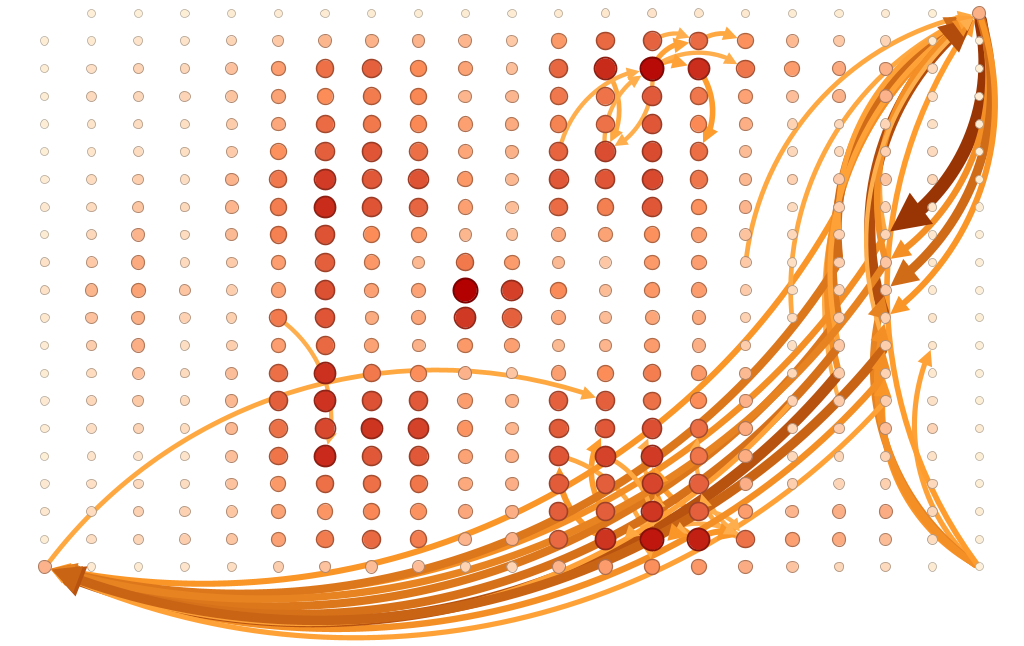
\includegraphics[width=\linewidth]{titleimage.png}
\end{figure}

\vfill

\begin{tabular}{@{}p{5cm} l}
Modul                    & SAN\\[2ex]
Autoren                  & Lukas Breiter\\
                         & Gian Truttmann\\
                         & Jessica Schmid\\[2ex]
Dozent                   & Michael Henninger\\[2ex]
Studiengang              & SG DSAI\\[2ex]
Semester                 & HS 2025\\[2ex]
Version / Abgabedatum    & 1.0 / 04.01.2026\\[4ex]
\multicolumn{2}{@{}l}{Fachhochschule Nordwestschweiz (FHNW)}
\end{tabular}

\clearpage

%%---ABSTRACT----------------------------------------------------------------------------
\selectlanguage{ngerman}
\thispagestyle{empty}
\section*{Abstract}
\noindent
\textit{Kurzbeschreibung des Berichts (max. ca. 150--200 W\"orter). Beschreibe Ziel, Daten/Material, Methode und wichtigste Ergebnisse in wenigen S\"atzen.}

\vspace{2ex}

\noindent\textbf{Keywords:} soziale Netzwerkanalyse, Graphen, Communities, Zentralit\"at, Link Prediction

\clearpage


%%---TABLE OF CONTENTS-------------------------------------------------------------------
\selectlanguage{ngerman}
\tableofcontents
\clearpage

\listoffigures
\listoftables

%%---TEXT--------------------------------------------------------------------------------
\pagenumbering{arabic}

\section{Exploratory Data Analysis (EDA)}

\subsection{Ziel und Kapitelrolle}
Dieses Kapitel liefert den einmaligen Überblick über Datensatz, Vorverarbeitung und zentrale Verteilungen. Ziel der EDA ist es, die Datenstruktur zu validieren, Kerndistributionen (Ereignisse, Pässe) zu charakterisieren und daraus belastbare Annahmen für die Netzwerk-Analysen abzuleiten.

\textbf{Analyseumfang:} Die EDA analysiert \emph{alle sieben Wettbewerbe} (England, Spanien, Deutschland, Frankreich, Italien, World Cup, European Championship) gemeinsam, um ein umfassendes Bild des Gesamtdatensatzes zu erhalten. In den nachfolgenden Kapiteln (LE3 ff.) werden dann einzelne Wettbewerbe fokussiert untersucht, um die Rechenkomplexität für detaillierte Netzwerkanalysen zu reduzieren.

\subsection{Datenbasis und Aufbereitung}
\begin{itemize}
  \item \textbf{Datenquellen:} Die Rohdaten liegen als JSON-Dateien in \texttt{data/} vor (Wettbewerbe, Spiele, Ereignisse, Teams, Spieler) und umfassen mehrere Wettbewerbe. Bezogen wurden sie von \cite{pappalardo-2019}. Dort findet sich auch eine sehr umfassende Variabelbeschreibung.
  \item \textbf{Robuster Import:} Unicode-Bereinigung und fehlerresistentes Einlesen (für grosse Event-Dateien ggf. Streaming). Fehlende Felder (z.\,B. Positionen) werden als \textit{NaN} geführt und in Auswertungen entsprechend behandelt.
  \item \textbf{Feature Engineering:} Aus Event-Positionen werden Start-/Endpunkte extrahiert und einfache Distanzmasse für Pässe berechnet. Für Zeitreihen werden Events pro Minute aggregiert; beide Halbzeiten beginnen jeweils bei Minute 0.
  \item \textbf{Ausschlüsse:} Ereignisse ohne ausreichende Positionsinformationen fliessen nicht in Distanzverteilungen ein.
\end{itemize}

\subsection{Wettbewerbe und Spiele}

\begin{figure}[htbp]
  \centering
  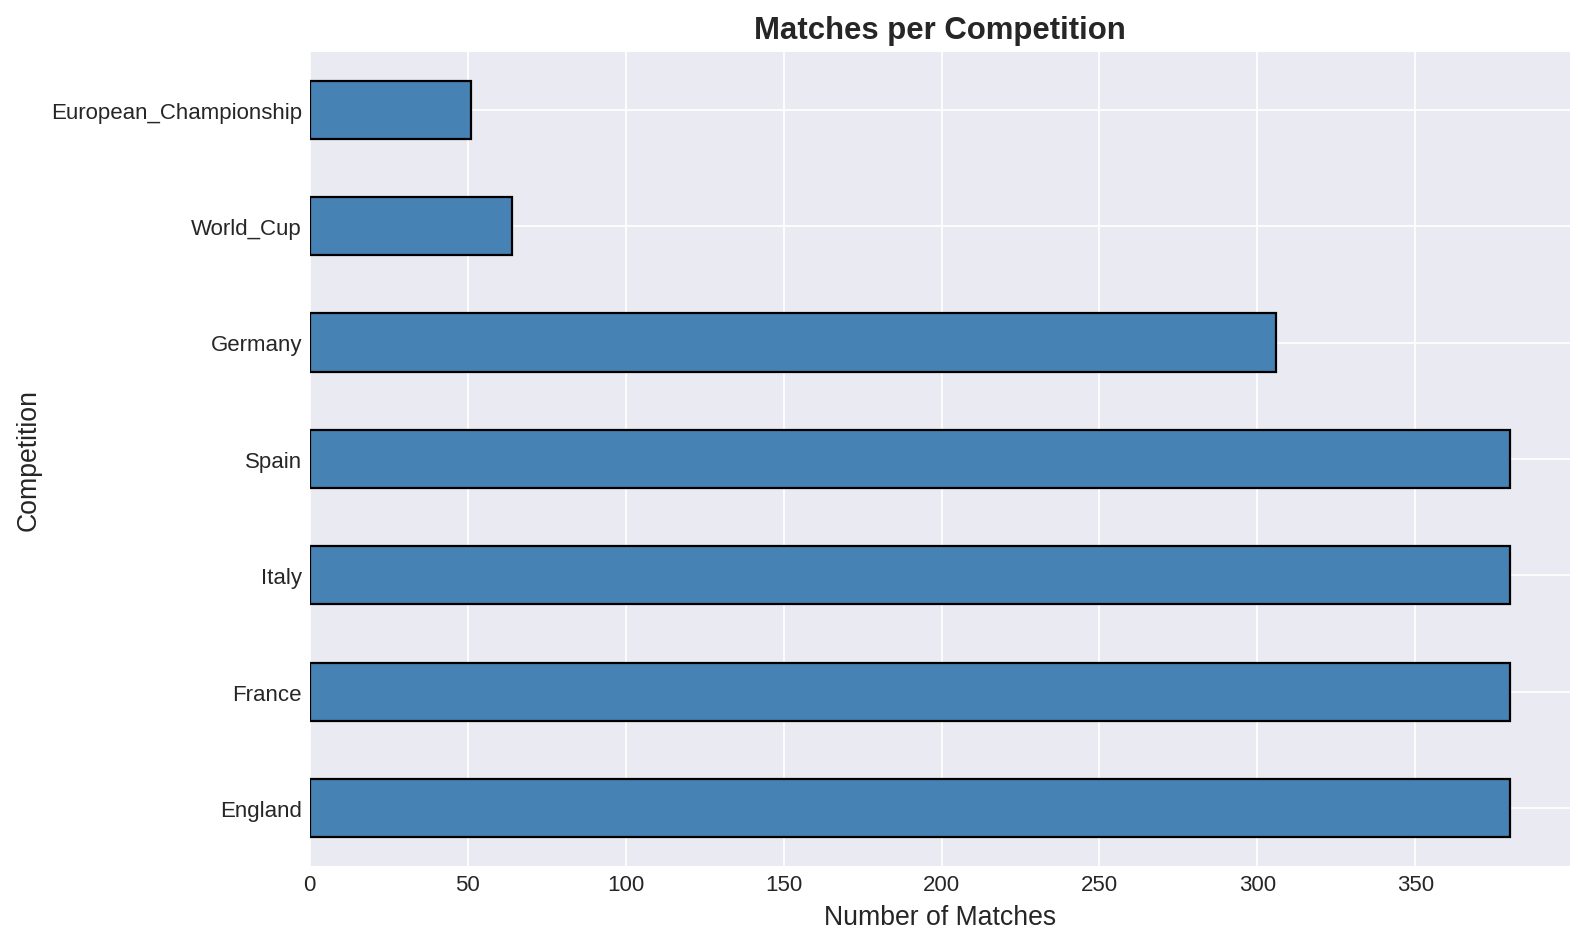
\includegraphics[width=0.85\linewidth]{figures/eda/matches_per_competition.png}
  \caption{Anzahl der Spiele pro Wettbewerb. Sowohl Liga-Wettbewerbe wie auch internationale Turniere}
  \label{fig:matches_per_competition}
\end{figure}

Der Datensatz umfasst mehrere europäische Top-Ligen sowie internationale Turniere. Abbildung~\ref{fig:matches_per_competition} zeigt die Verteilung der Spiele über die Wettbewerbe. Unterschiede in der Spielanzahl spiegeln Ligaformate (z.\,B. 38 Spieltage) und Turnierlängen wider.

Ergänzend zeigt Abbildung~\ref{fig:events_by_competition} die Anzahl der Ereignisse pro Wettbewerb. Erwartungsgemäss skaliert die Eventanzahl stark mit der Anzahl Spiele. Die Liga-Wettbewerbe (England, Spanien, Frankreich, Italien) weisen jeweils ca. 650{,}000 Events auf (ca. 1{,}710 Events pro Match), während Deutschland mit ca. 530{,}000 Events (ca. 1{,}730 Events/Match) und die Turniere World Cup und European Championship mit ca. 130{,}000 bzw. 100{,}000 Events eine geringere Gesamtzahl aufweisen. Dies bildet eine robuste Basis für detaillierte Netzwerkanalysen.

\begin{figure}[htbp]
  \centering
  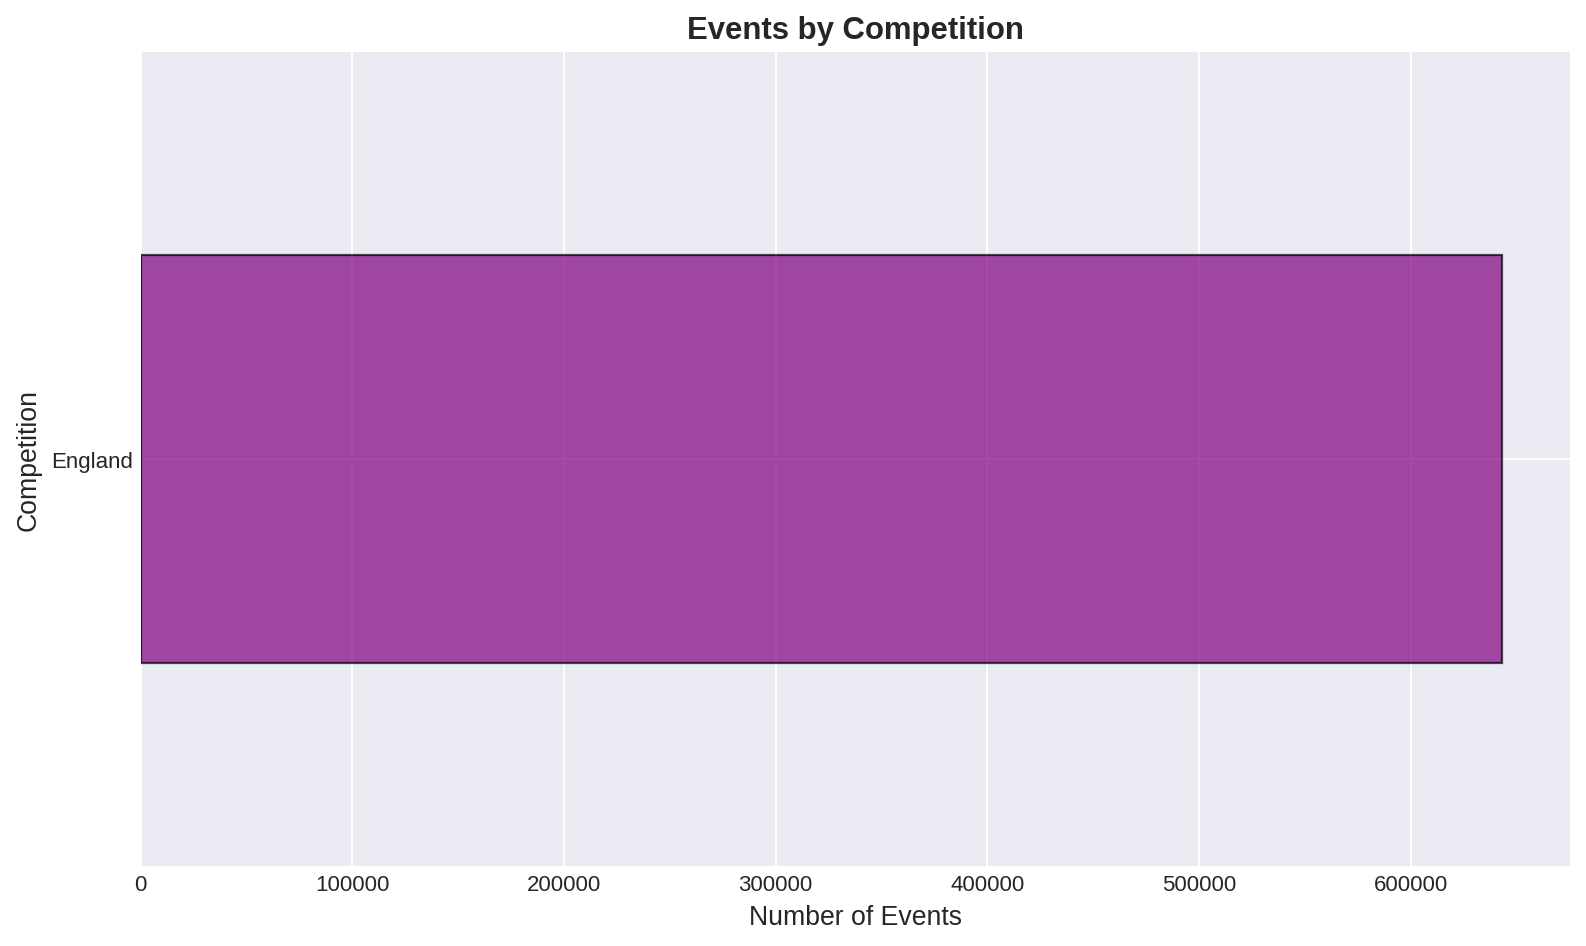
\includegraphics[width=0.85\linewidth]{figures/eda/events_by_competition.png}
  \caption{Anzahl der Events pro Wettbewerb. Stark abhängig vom Format des Turniers.}
  \label{fig:events_by_competition}
\end{figure}

Zur Veranschaulichung der Match-Metadaten zeigt Tabelle~\ref{tab:matches_sample} eine zufällige Stichprobe von 5 Spielen (\texttt{df.sample(5)} auf dem Match-DataFrame):

\begin{table}[htbp]
\centering
\small
\begin{tabularx}{\linewidth}{lllXXl}
\toprule
Team 1 & Team 2 & Score & Date & Venue & Duration \\
\midrule
Huddersfield Town & Crystal Palace & 0 - 2 & March 17, 2018 at 4:00:00 PM GMT+1 & The John Smith's Stadium & Regular \\ \addlinespace
Manchester United & Crystal Palace & 4 - 0 & Sept 30, 2017 at 4:00:00 PM GMT+2 & Old Trafford & Regular \\ \addlinespace
Everton & Southampton & 1 - 1 & May 5, 2018 at 6:30:00 PM GMT+2 & Goodison Park & Regular \\ \addlinespace
Everton & Manchester United & 0 - 2 & Jan 1, 2018 at 6:30:00 PM GMT+1 & Goodison Park & Regular \\ \addlinespace
Stoke City & Liverpool & 0 - 3 & Nov 29, 2017 at 9:00:00 PM GMT+1 & Bet365 Stadium & Regular \\
\bottomrule
\end{tabularx}
\caption{Beispiele von 5 zufällig ausgewählten Spielen aus dem Gesamtdatensatz mit Spielbezeichnung, Datum, Austragungsort und Spieldauer.}
\label{tab:matches_sample}
\end{table}

\subsection{Ereignisse: Typen und zeitliche Muster}

Die Event-Typen sind über IDs und Labels definiert; Tabelle~\ref{tab:event_types} dokumentiert diese Zuordnung und dient in späteren Kapiteln als Referenz für Filter und Aggregationen.

\begin{table}[htbp]
\centering
\small
\setlength{\tabcolsep}{3pt}
\begin{tabular}{lrrll}

\toprule
 & event & subevent & event\_label & subevent\_label \\
\midrule
0 & 1 & 10 & Duel & Air duel \\
1 & 1 & 11 & Duel & Ground attacking duel \\
2 & 1 & 12 & Duel & Ground defending duel \\
3 & 1 & 13 & Duel & Ground loose ball duel \\
4 & 2 & 20 & Foul & Foul \\
5 & 2 & 21 & Foul & Hand foul \\
6 & 2 & 22 & Foul & Late card foul \\
7 & 2 & 23 & Foul & Out of game foul \\
8 & 2 & 24 & Foul & Protest \\
9 & 2 & 25 & Foul & Simulation \\
10 & 2 & 26 & Foul & Time lost foul \\
11 & 2 & 27 & Foul & Violent Foul \\
12 & 3 & 30 & Free Kick & Corner \\
13 & 3 & 31 & Free Kick & Free Kick \\
14 & 3 & 32 & Free Kick & Free kick cross \\
15 & 3 & 33 & Free Kick & Free kick shot \\
16 & 3 & 34 & Free Kick & Goal kick \\
17 & 3 & 35 & Free Kick & Penalty \\
18 & 3 & 36 & Free Kick & Throw in \\
19 & 4 & 40 & Goalkeeper leaving line & Goalkeeper leaving line \\
20 & 5 & 50 & Interruption & Ball out of the field \\
21 & 5 & 51 & Interruption & Whistle \\
22 & 6 & 60 & Offside & Offside \\
23 & 7 & 70 & Others on the ball & Acceleration \\
24 & 7 & 71 & Others on the ball & Clearance \\
25 & 7 & 72 & Others on the ball & Touch \\
26 & 8 & 80 & Pass & Cross \\
27 & 8 & 81 & Pass & Hand pass \\
28 & 8 & 82 & Pass & Head pass \\
29 & 8 & 83 & Pass & High pass \\
30 & 8 & 84 & Pass & Launch \\
31 & 8 & 85 & Pass & Simple pass \\
32 & 8 & 86 & Pass & Smart pass \\
33 & 9 & 90 & Save attempt & Reflexes \\
34 & 9 & 91 & Save attempt & Save attempt \\
35 & 10 & 100 & Shot & Shot \\
\bottomrule
\end{tabular}
\caption{Vollständige Übersicht der Ereignistypen und Subtypen im Datensatz. Die Spalten geben die Event-ID und Subevent-ID sowie deren sprachliche Bezeichnung an.}
\label{tab:event_types}
\end{table}

Die Analyse der Ereignistypen in Abbildung~\ref{fig:event_types_top15} zeigt erwartungsgemäss, dass Pässe die häufigste Aktion darstellen, gefolgt von Duellen und Ballkontakten. Diese Dominanz von Passereignissen motiviert den den Schwerpunkt in der analyse später auf ein Passnetzwerke zu legen.

\begin{figure}[htbp]
  \centering
  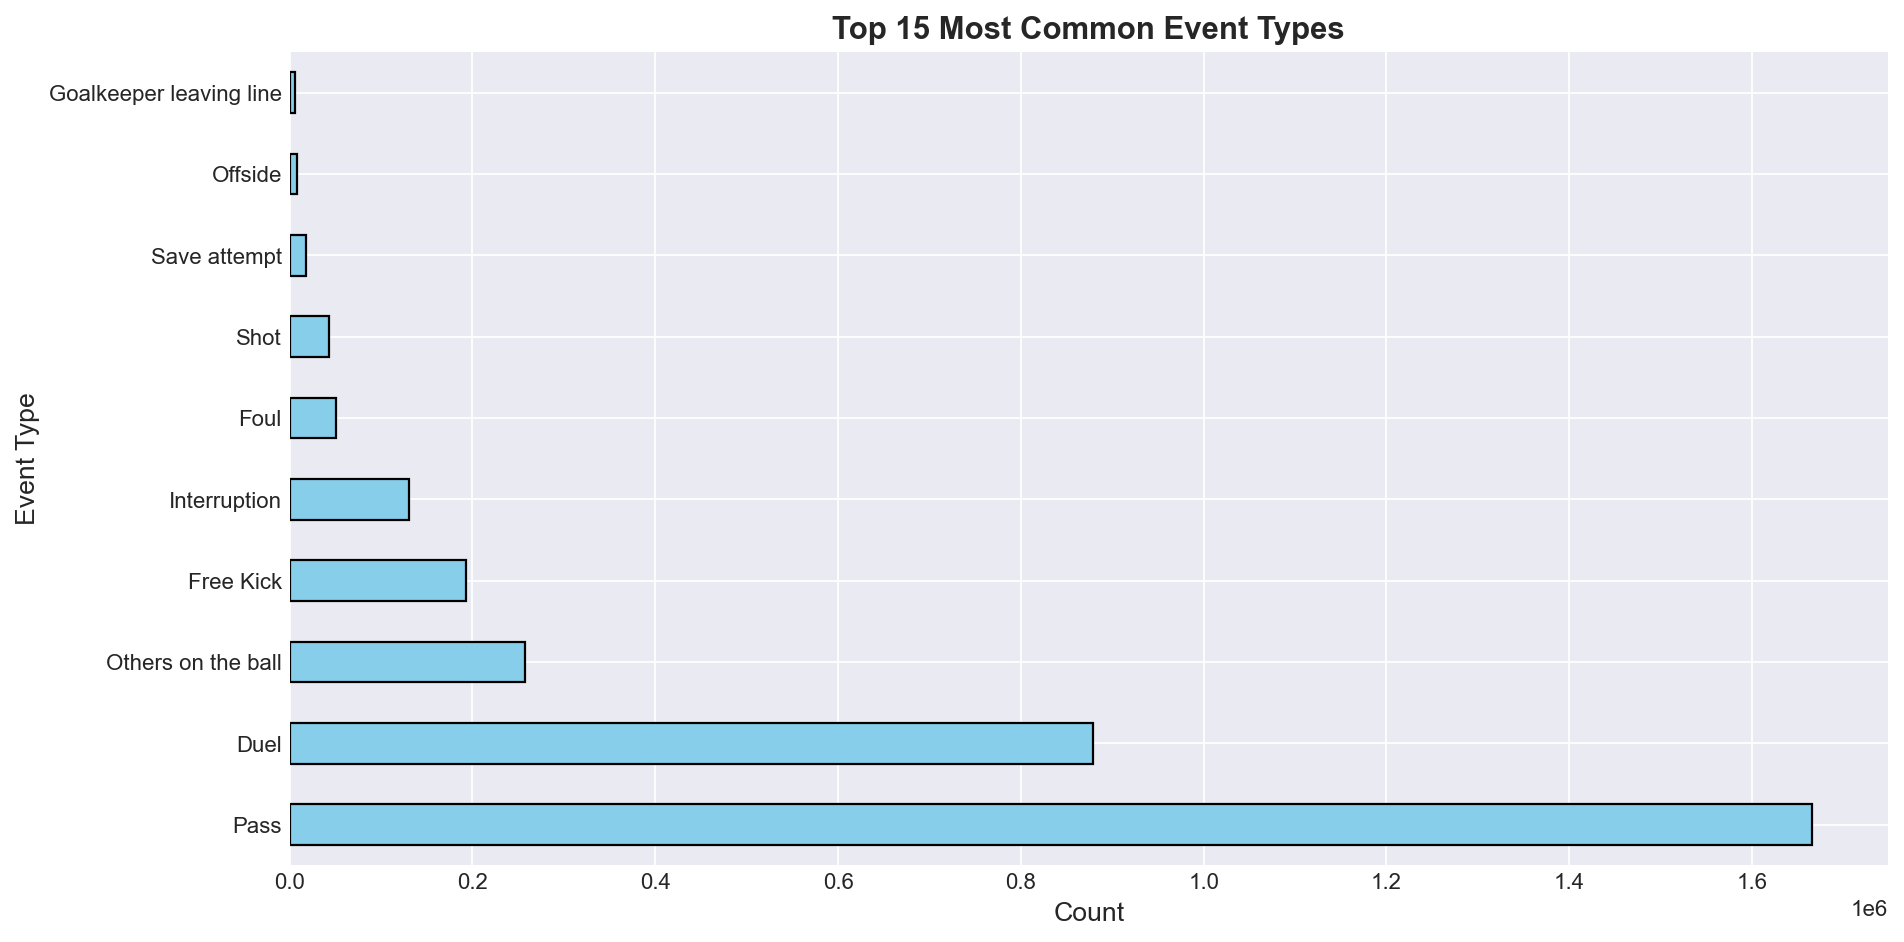
\includegraphics[width=0.9\linewidth]{figures/eda/event_types_top15.png}
  \caption{Top 15 Ereignistypen über alle Wettbewerbe. Pässe dominieren klar das Spielgeschehen.}
  \label{fig:event_types_top15}
\end{figure}

Die zeitliche Verteilung der Ereignisse über den Spielverlauf (Abbildung~\ref{fig:events_per_minute}) zeigt erhöhte Aktivität zu Beginn beider Halbzeiten sowie einen Abfall gegen Ende der Halbzeiten.

\begin{figure}[htbp]
  \centering
  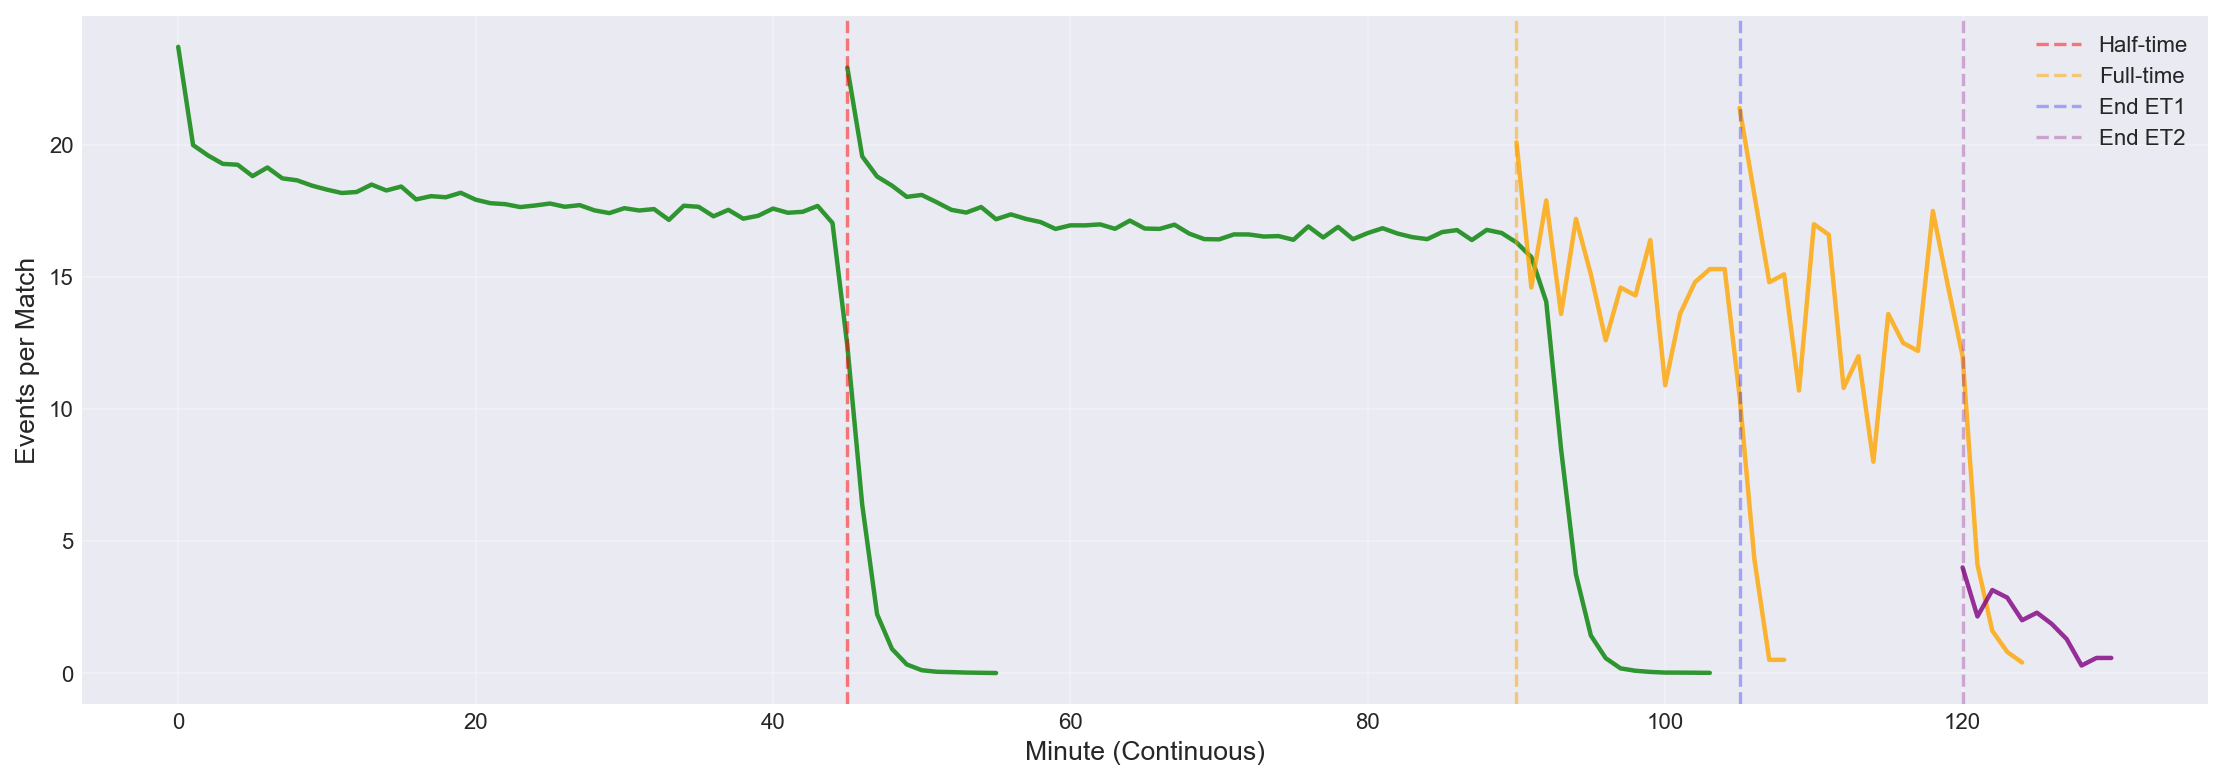
\includegraphics[width=0.9\linewidth]{figures/eda/events_per_minute_normalized.png}
  \caption{Ereignisse pro Spielminute. Deutlich erkennbar sind erhöhte Aktivität zu Spielbeginn und der Rückgang in der Schlussphase.}
  \label{fig:events_per_minute}
\end{figure}

Auf aggregierter Ebene ist die Datenabdeckung über die reguläre Spielzeit ausgeglichen: Abbildung~\ref{fig:events_by_period} zeigt nahezu identische Event-Zahlen in der ersten und zweiten Halbzeit (je ca. \num{1.62e6} Events).

\begin{figure}[htbp]
  \centering
  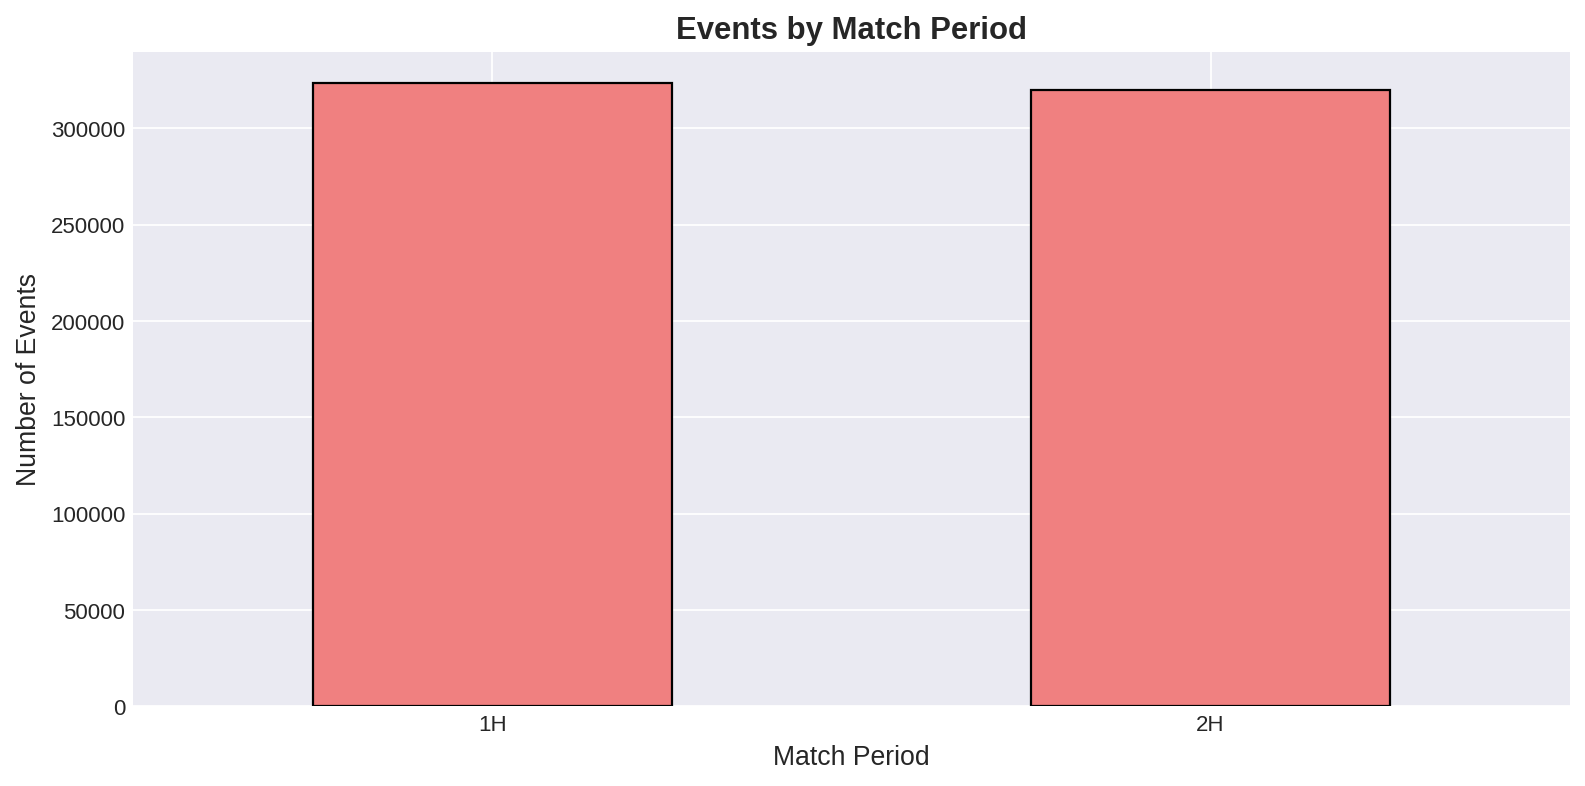
\includegraphics[width=0.7\linewidth]{figures/eda/events_by_period.png}
  \caption{Events nach Spielperiode. In der vorliegenden Auswertung sind beide \textbf{H}albzeiten mit je über \num{1.62e6} Events nahezu gleich stark vertreten. \textbf{E}xtended 1 / 2 sowie \textbf{P}enaly kommen bedeutend seltener vor (10 / 10 / 7)}
  \label{fig:events_by_period}
\end{figure}

Für Passereignisse zeigt sich jedoch ein leichter Halbzeiteffekt (Abbildung~\ref{fig:passes_by_period}): In der ersten Halbzeit werden mehr Pässe gespielt, die Passgenauigkeit ist minimal höher (82.99\% vs. 82.06\%) und die durchschnittliche Passdistanz praktisch unverändert (24.69 vs. 24.54). Dies passt zu Effekten wie Ermüdung, Spielstandmanagement oder erhöhtem Druck in Halbzeit 2.

\begin{figure}[htbp]
  \centering
  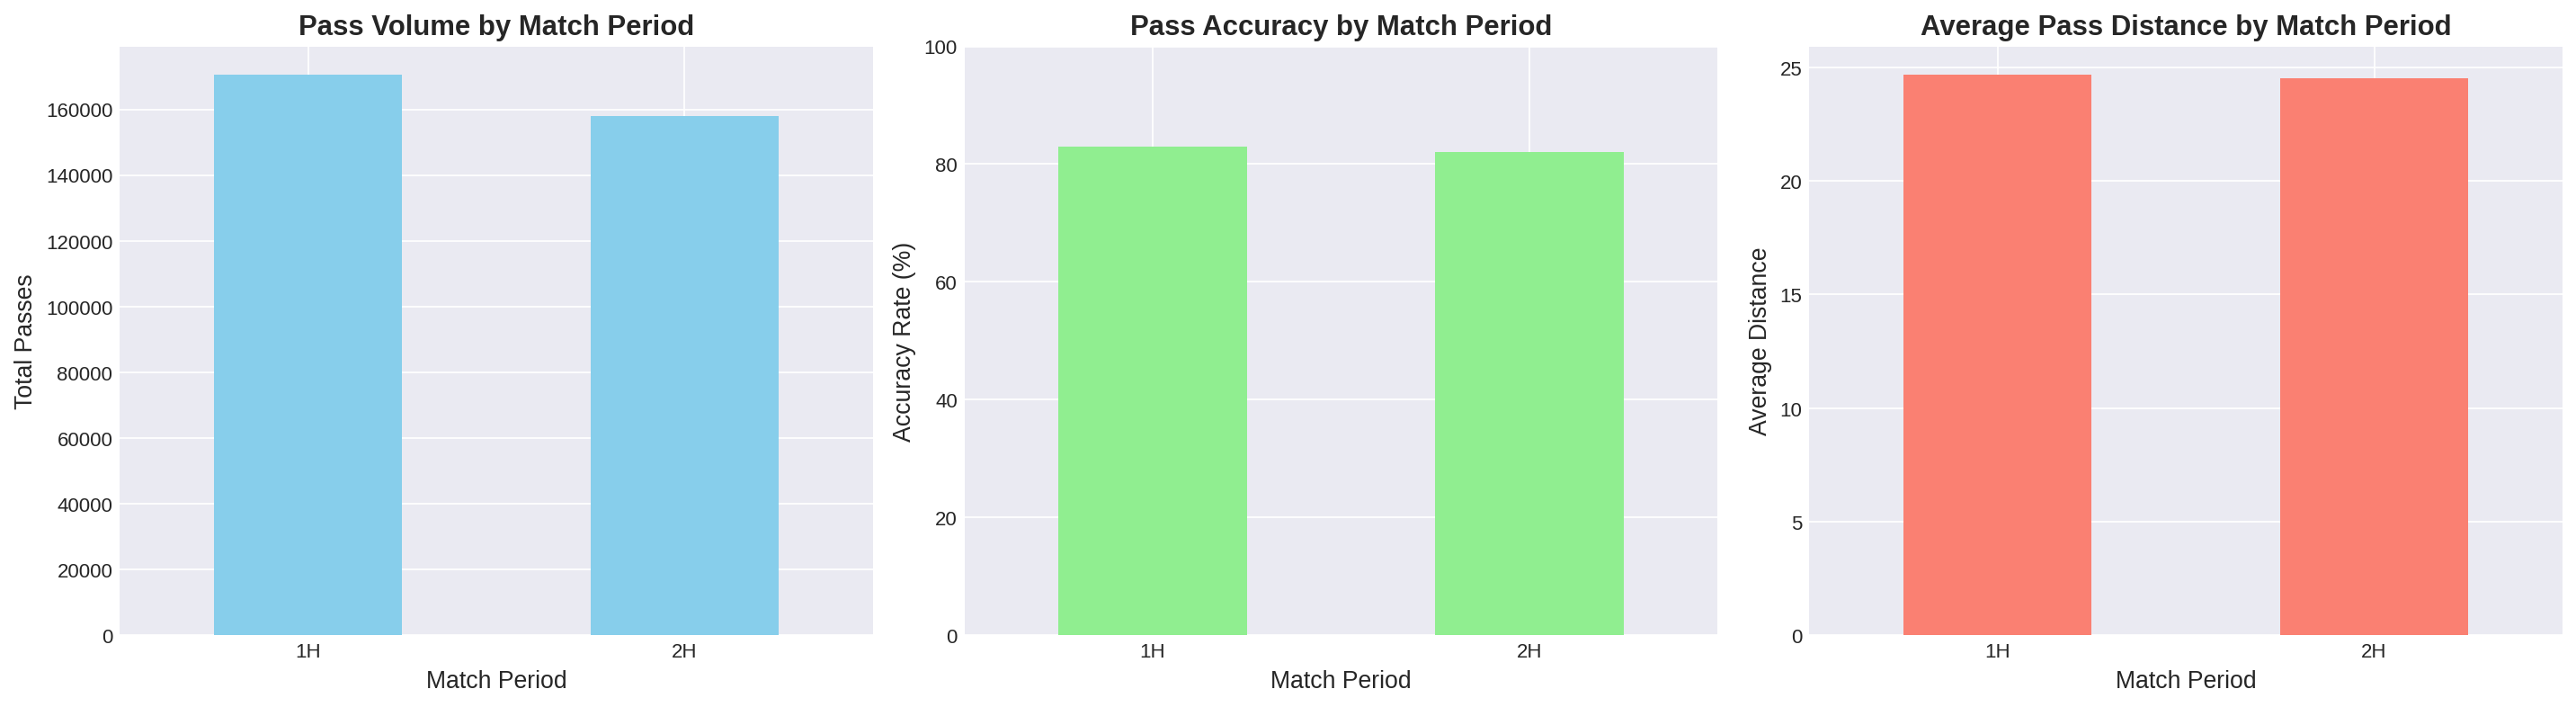
\includegraphics[width=\linewidth]{figures/eda/passes_by_period.png}
  \caption{Passvolumen, Passgenauigkeit und durchschnittliche Passdistanz nach Matchperiode. In dieser Auswertung werden in Halbzeit 1 mehr Pässe gespielt (+7.4\%), bei sehr ähnlicher Genauigkeit und Distanz.}
  \label{fig:passes_by_period}
\end{figure}

Während der Verlängerungsphasen ist eine Zunahme der Passlänge bei gleichzeitig abnehmender Genauigkeit zu verzeichnen. Diese Verhaltensweise lässt sich durch eine aggressivere Spielweise erklären, mit der versucht wird, ein Penalty-Szenario zu vermeiden. Ausserdem wird mit diesen Pässen hauptsächlich das Ziel verfolgt, Fehler zu vermeiden, indem eine möglichst grosse Distanz zum eigenen Tor geschaffen wird (A. Scheifele, persönliche Kommunikation, 30. Dezember 2025).

\subsection{Pass-Analyse: Zentrale Akteure und räumliche Verteilung}

Pässe bilden neben Teams \& Spielen das Rückgrat der späteren Netzwerkanalyse. Abbildung~\ref{fig:top_passers} identifiziert die aktivsten Passgeber. Diese Spieler sind Kandidaten für zentrale Knoten (hohe Degree- und Betweennesszentralität), da sie als Verteiler im Spielaufbau fungieren.

\begin{figure}[htbp]
  \centering
  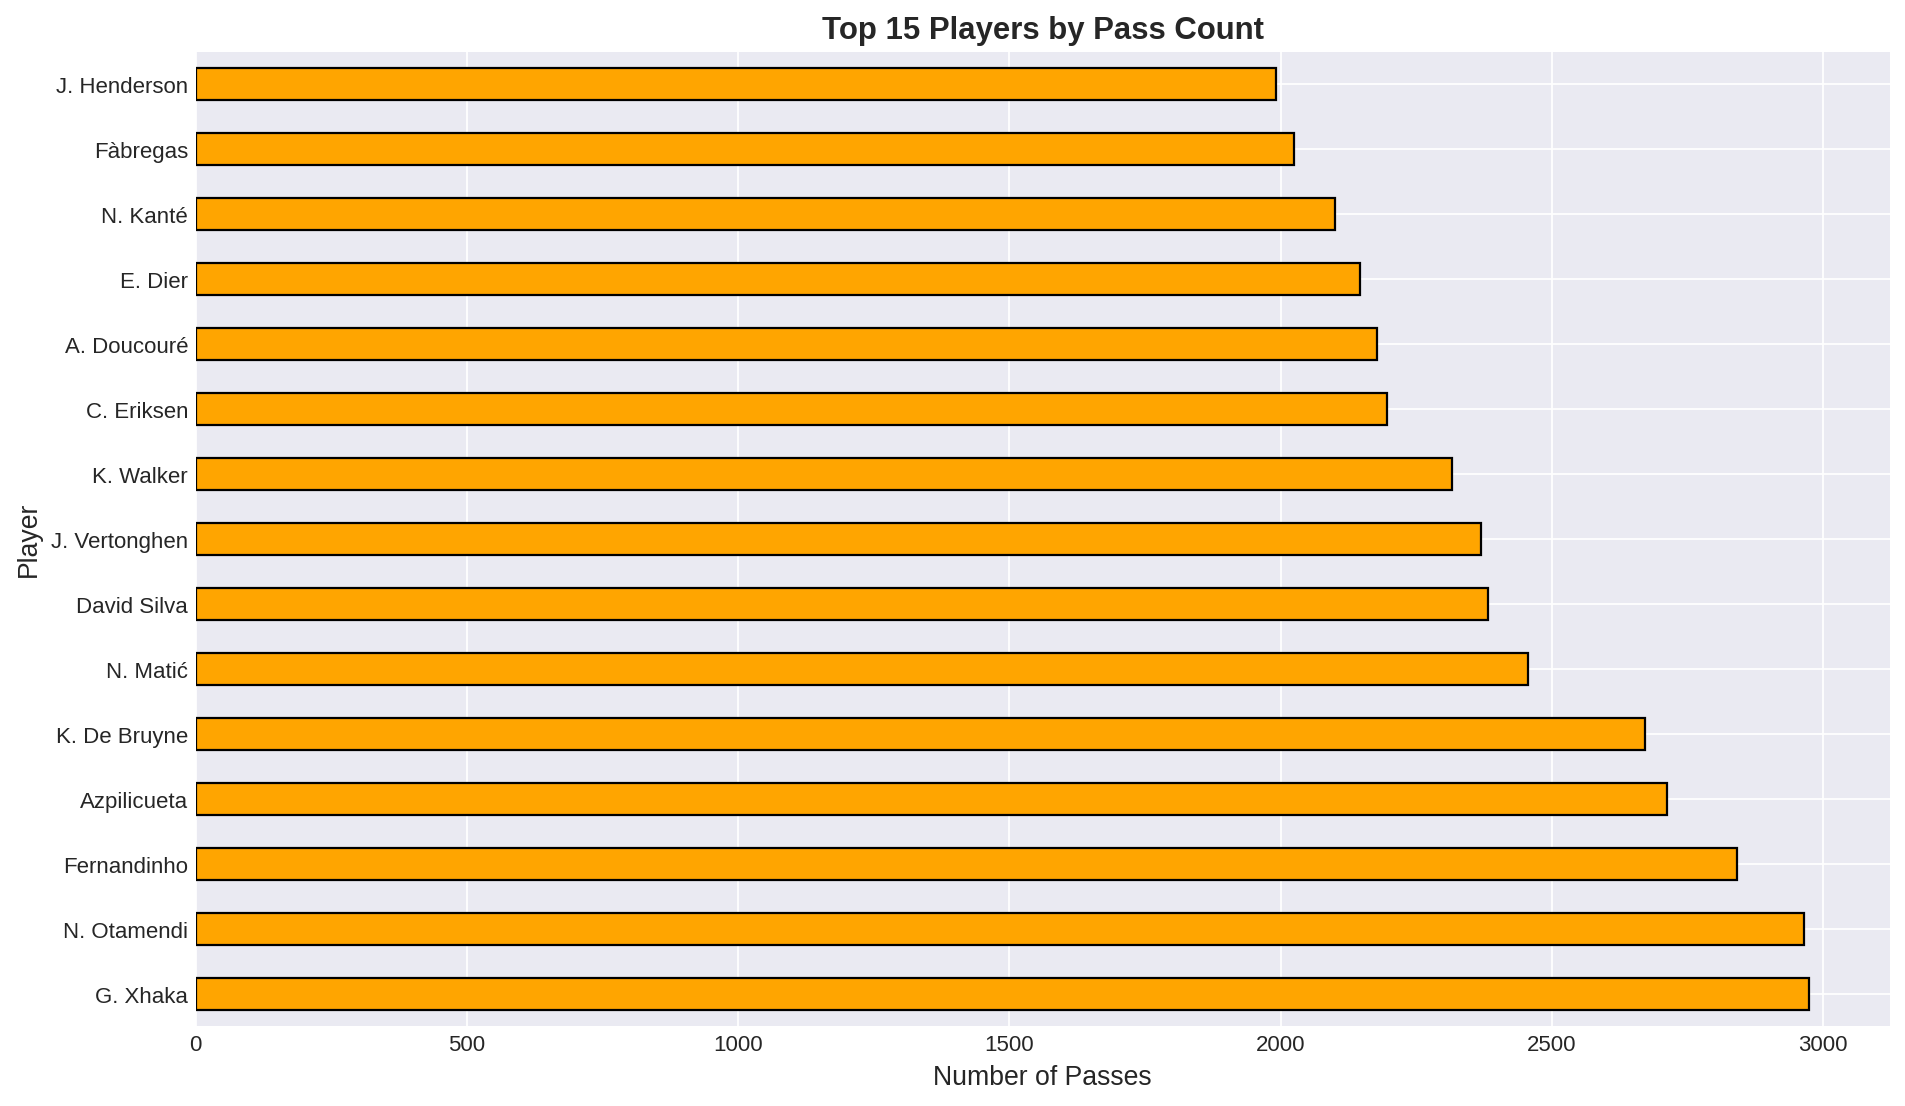
\includegraphics[width=0.85\linewidth]{figures/eda/top_passers.png}
  \caption{Top 15 Spieler nach Anzahl der Pässe. Diese Spieler sind später als zentrale Knoten in den Passnetzwerken zu erwarten.}
  \label{fig:top_passers}
\end{figure}

\begin{figure}[htbp]
  \centering
  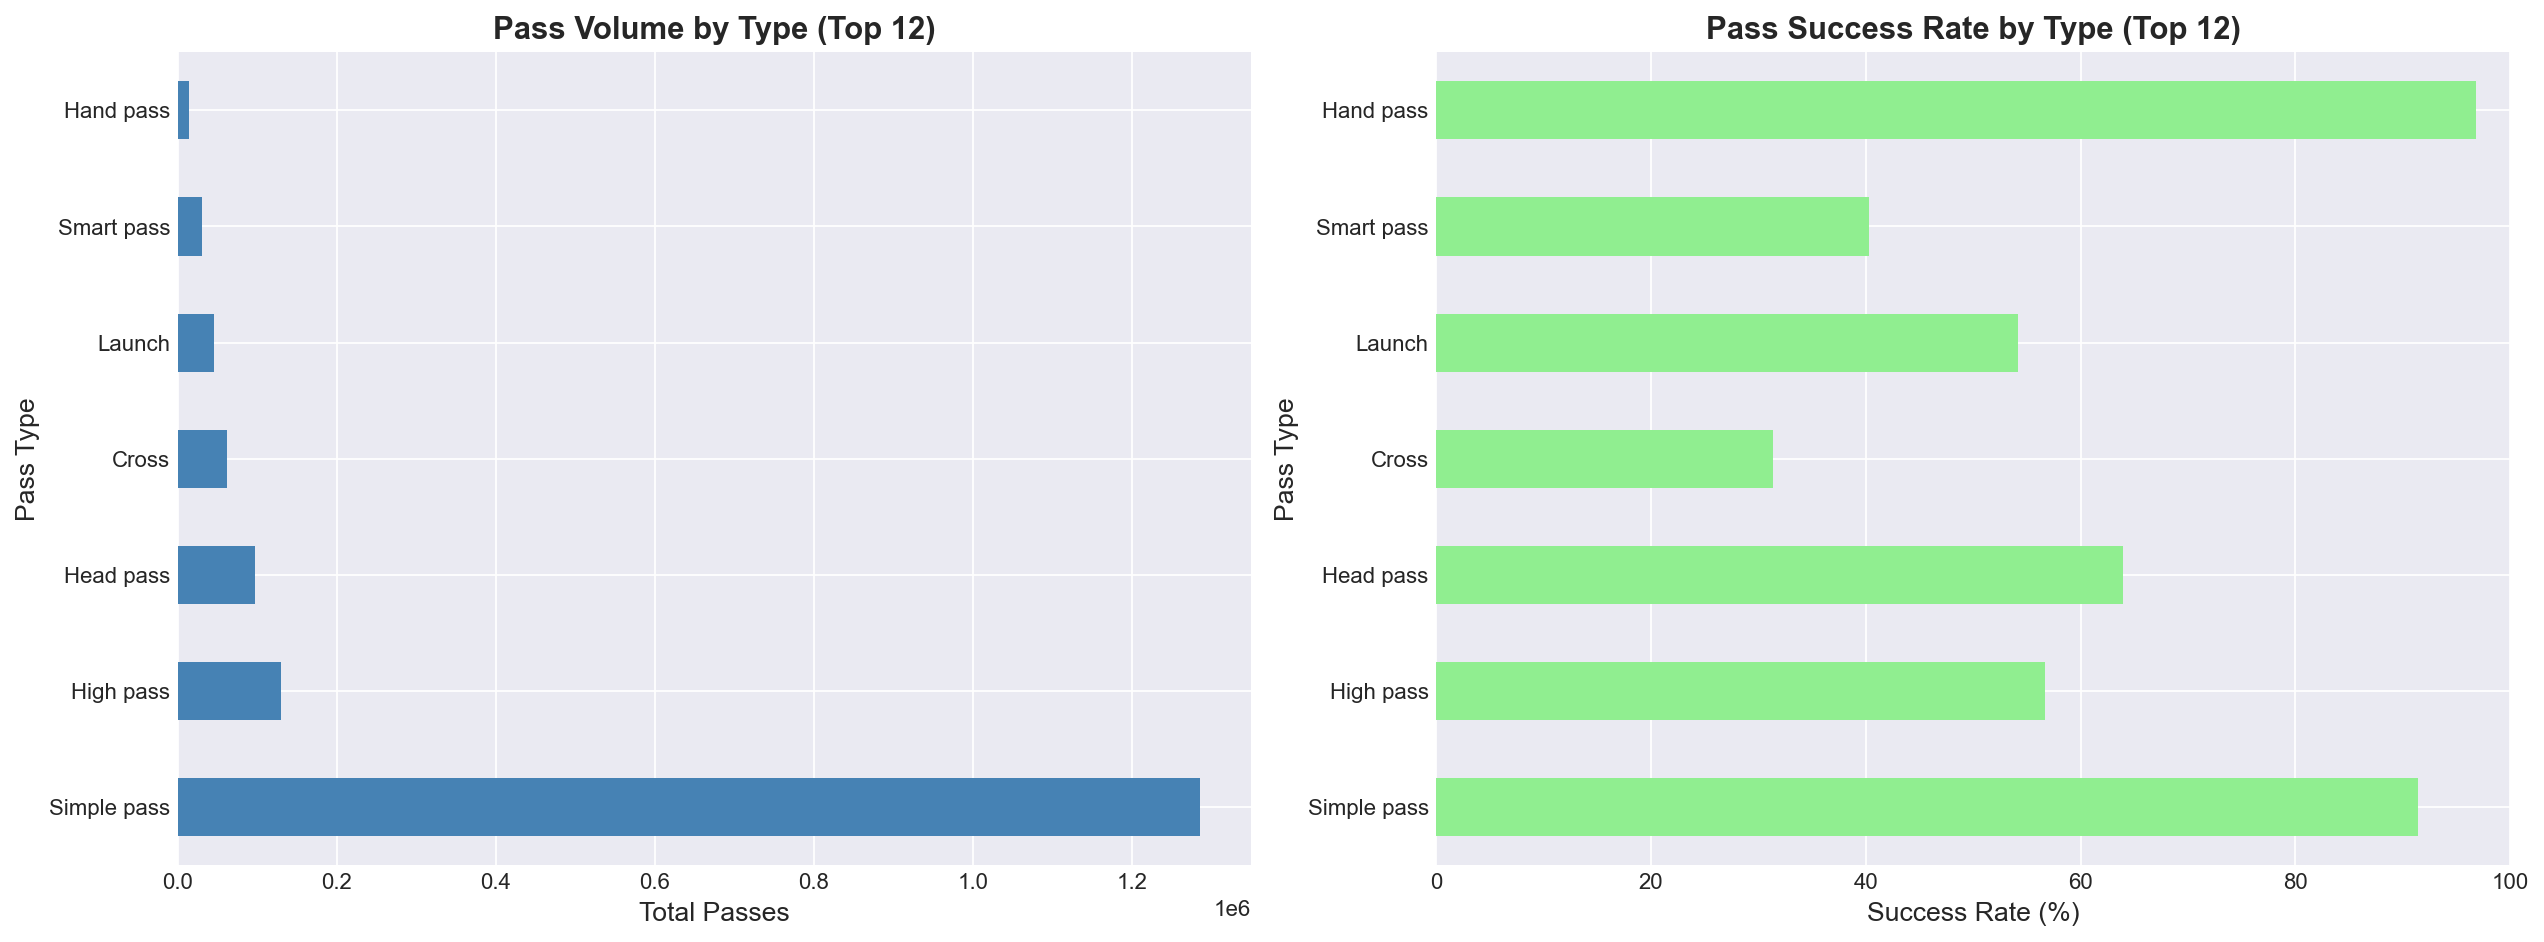
\includegraphics[width=\linewidth]{figures/eda/pass_types_analysis.png}
  \caption{Passvolumen (links) und Passgenauigkeit (rechts) nach Passtyp. Einfache Pässe dominieren das Volumen bei hoher Genauigkeit; Flanken und Smart Passes sind seltener und deutlich ungenauer. Handpässe verzeichnen aufgrund der manuellen Ballkontrolle und ihrer exklusiven Anwendung durch den Torhüter die höchste Präzision.}
  \label{fig:pass_types_analysis}
\end{figure}

Sowohl räumlichen Mustern als auch die Struktur nach Passtyp sind zentral für die Interpretation von Netzwerkkanten: Abbildung~\ref{fig:pass_types_analysis} zeigt, dass einfache Pässe den Grossteil des Volumens ausmachen (ca. 76\% aller Pässe) und zugleich eine sehr hohe Genauigkeit aufweisen (> 91\%). Risikoreichere Pässe (Flanken, Smart Passes) treten seltener auf und haben deutlich niedrigere Erfolgsraten (z.\,B. Flanken ca. 30.71\%). Für die spätere Netzwerkanalyse von Passlängen bedeutet dies: Gewichte werden stark durch kurze, sichere Verbindungen dominiert, während wenige riskante Kanten eher spielentscheidende Situationen abbilden.

Eine detaillierte räumliche Analyse der Pässe (Abbildung~\ref{fig:pass_distance_analysis}) liefert mehrere wichtige Erkenntnisse:
\begin{itemize}
  \item Die \textbf{Passlängenverteilung} (oben links) zeigt eine rechtssteile Verteilung mit Median bei ca. 15 Einheiten, was kurzen bis mittellangen Pässen entspricht. Lange Bälle sind seltener.
  \item Die \textbf{Passlängen nach Typ} (oben rechts) verdeutlichen erwartbare Unterschiede: Lange Bälle und Flanken weisen deutlich grössere Distanzen auf als einfache Zuspiele.
  \item Die \textbf{Heatmaps} (unten) für Pass-Ursprung und -Ziel zeigen die räumliche Konzentration: Viele Pässe starten und enden im Mittelfeld sowie in defensiven Bereichen, während Pässe im gegnerischen Strafraum seltener sind.
\end{itemize}

\begin{figure}[htbp]
  \centering
  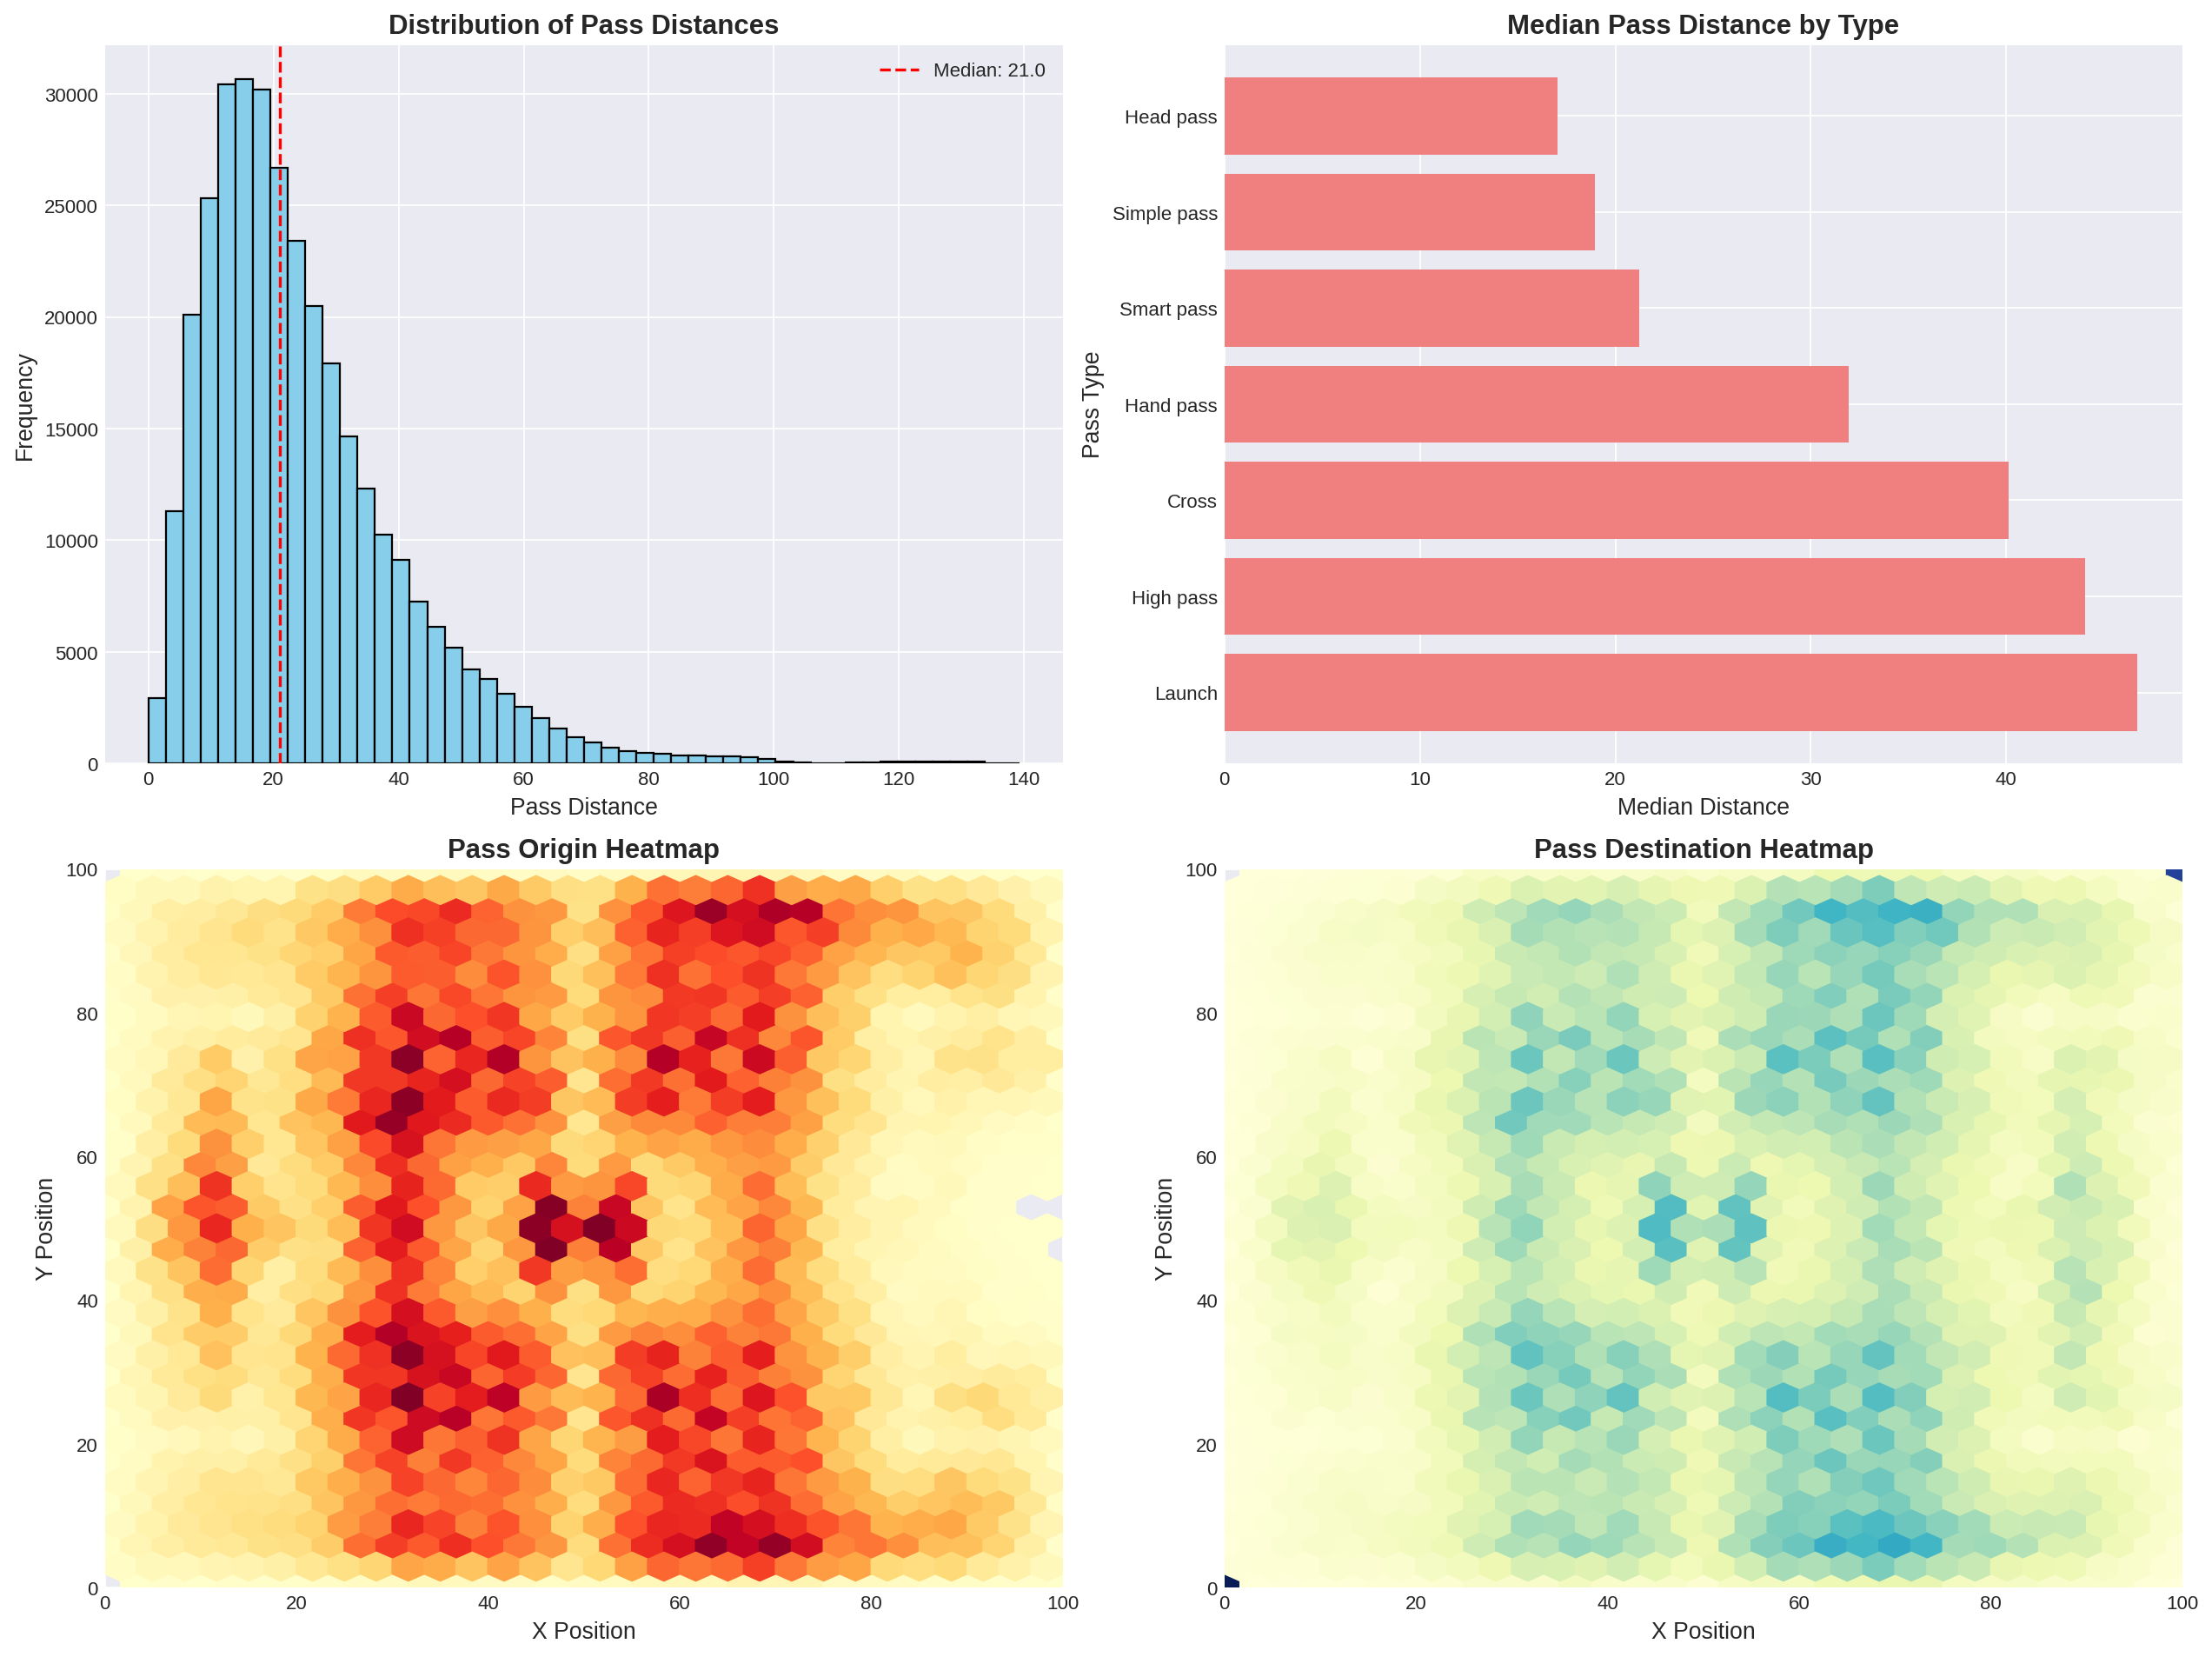
\includegraphics[width=\linewidth]{figures/eda/pass_distance_analysis.png}
  \caption{Umfassende Analyse der Passeigenschaften. \textbf{Oben links:} Verteilung der Passlängen mit Median-Markierung. \textbf{Oben rechts:} Median-Passlänge nach Passtyp (z.\,B. lange Bälle vs. kurze Zuspiels). \textbf{Unten:} Heatmaps für Pass-Ursprung (links) und Pass-Ziel (rechts), visualisiert auf normalisierten Spielfeldkoordinaten.}
  \label{fig:pass_distance_analysis}
\end{figure}

Abbildung~\ref{fig:network_metrics_sample} illustriert die Rolleninterpretation einfacher Zentralitätskonzepte (Degreezentralität in diesem Fall) in einem Beispielspiel: Spieler oberhalb der Diagonalen erhalten mehr Pässe als sie spielen (Zielspieler), Spieler unterhalb verteilen mehr (Aufbauspieler), und Spieler nahe der Diagonalen sind ausgeglichen. Generell können wir erkennen: wer mehr Pässe bekommt, vergibt auch mehr.

\begin{figure}[htbp]
  \centering
  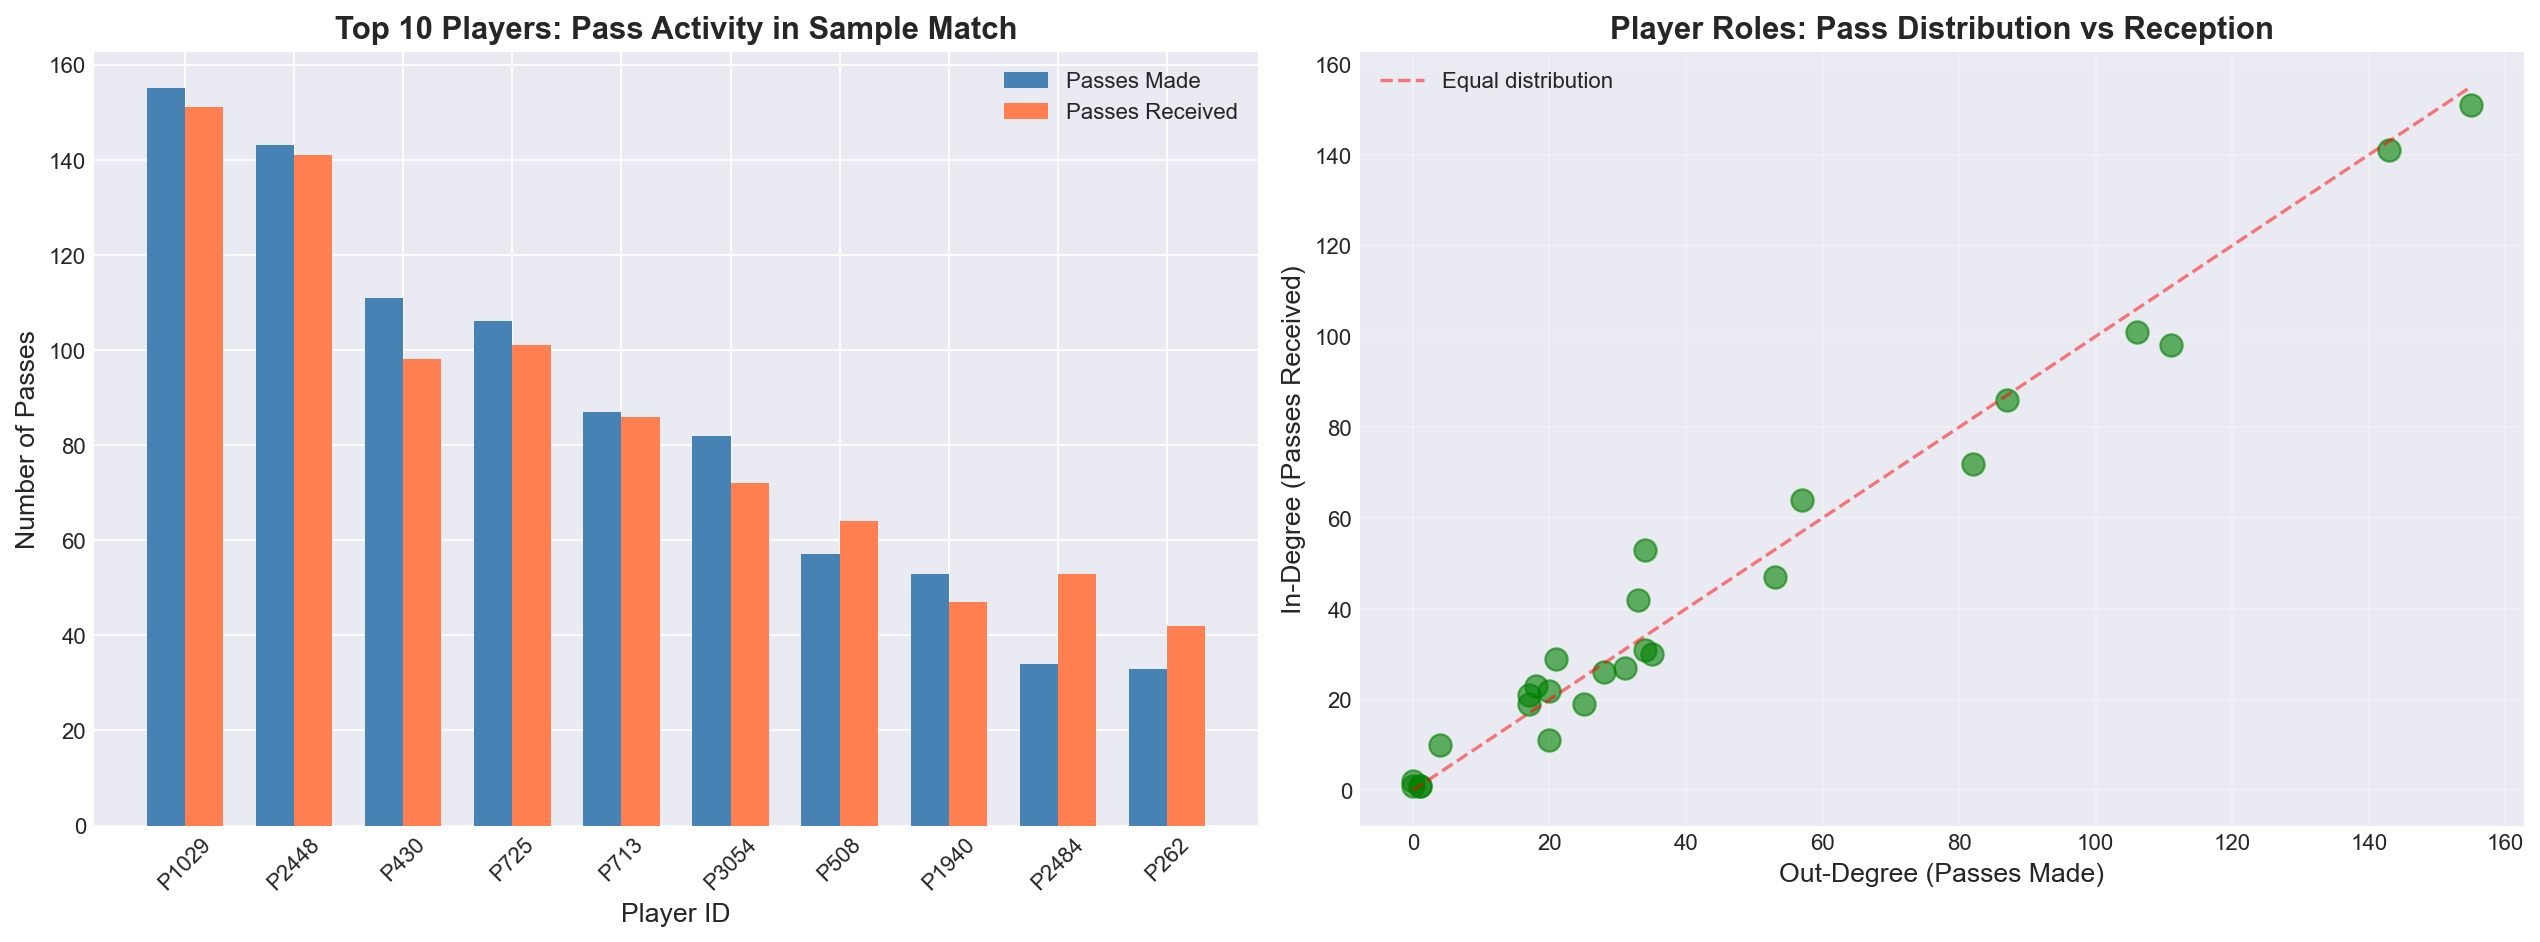
\includegraphics[width=\linewidth]{figures/eda/network_metrics_sample.png}
  \caption{Passverhältniss in einem Sample-Match: (links) Top-10 Spieler nach Passvolumen (gespielt vs. empfangen), (rechts) Out-Degree vs. In-Degree mit Referenzlinie $y=x$ zur Rolleninterpretation.}
  \label{fig:network_metrics_sample}
\end{figure}

Um die spätere Netzwerkkonstruktion zu illustrieren, zeigt Tabelle~\ref{tab:pass_network_sample} einen Ausschnitt aus einem berechneten Passnetzwerk eines Beispielspiels (Match-ID 2500004). Die Kanten sind Passverbindungen, gewichtet nach \textit{pass\_count}; zusätzlich ist die mittlere Passdistanz angegeben.

\begin{table}[htbp]
\centering
\small
\setlength{\tabcolsep}{4pt}
\begin{tabular}{lrrrrll}
\toprule
 & passer\_id & receiver\_id & pass\_count & avg\_distance & passer\_name & receiver\_name \\
\midrule
0 & 3324 & 8625.000000 & 1 & 4.123106 & Álvaro Morata & V. Moses \\
1 & 3350 & 3324.000000 & 1 & 13.038405 & Fàbregas & Álvaro Morata \\
2 & 3350 & 3360.000000 & 6 & 20.523277 & Fàbregas & Pedro \\
3 & 3350 & 3429.000000 & 3 & 25.654240 & Fàbregas & T. Courtois \\
4 & 3350 & 8032.000000 & 1 & 26.627054 & Fàbregas & Marcos Alonso \\
5 & 3350 & 8495.000000 & 3 & 12.648930 & Fàbregas & D. Drinkwater \\
6 & 3350 & 8625.000000 & 2 & 21.530491 & Fàbregas & V. Moses \\
7 & 3350 & 14748.000000 & 3 & 9.815600 & Fàbregas & A. Rüdiger \\
8 & 3350 & 25553.000000 & 9 & 18.920233 & Fàbregas & Azpilicueta \\
9 & 3350 & 25707.000000 & 1 & 17.804494 & Fàbregas & E. Hazard \\
\bottomrule
\end{tabular}
\caption{Ausschnitt eines Passnetzwerks: erste 10 Passverbindungen eines Beispielspiels (Match-ID 2500004) mit Anzahl der Pässe, mittlerer Distanz und Spielernamen.}
\label{tab:pass_network_sample}
\end{table}

\subsection{Wettbewerbsvergleich}

Die aggregierten Pass-Statistiken nach Wettbewerb (Abbildung~\ref{fig:competition_pass_stats}) ermöglichen einen direkten Vergleich der Spielstile: Volumen (Anzahl der Pässe), Genauigkeit (Erfolgsquote) und durchschnittliche Passlänge variieren zwischen den Ligen und Turnieren. Solche Unterschiede können auf taktische Präferenzen, Spieltempo oder die Qualität der Teams hindeuten und werden sich in den strukturellen Eigenschaften der daraus generierten Netzwerke widerspiegeln.

\begin{figure}[htbp]
  \centering
  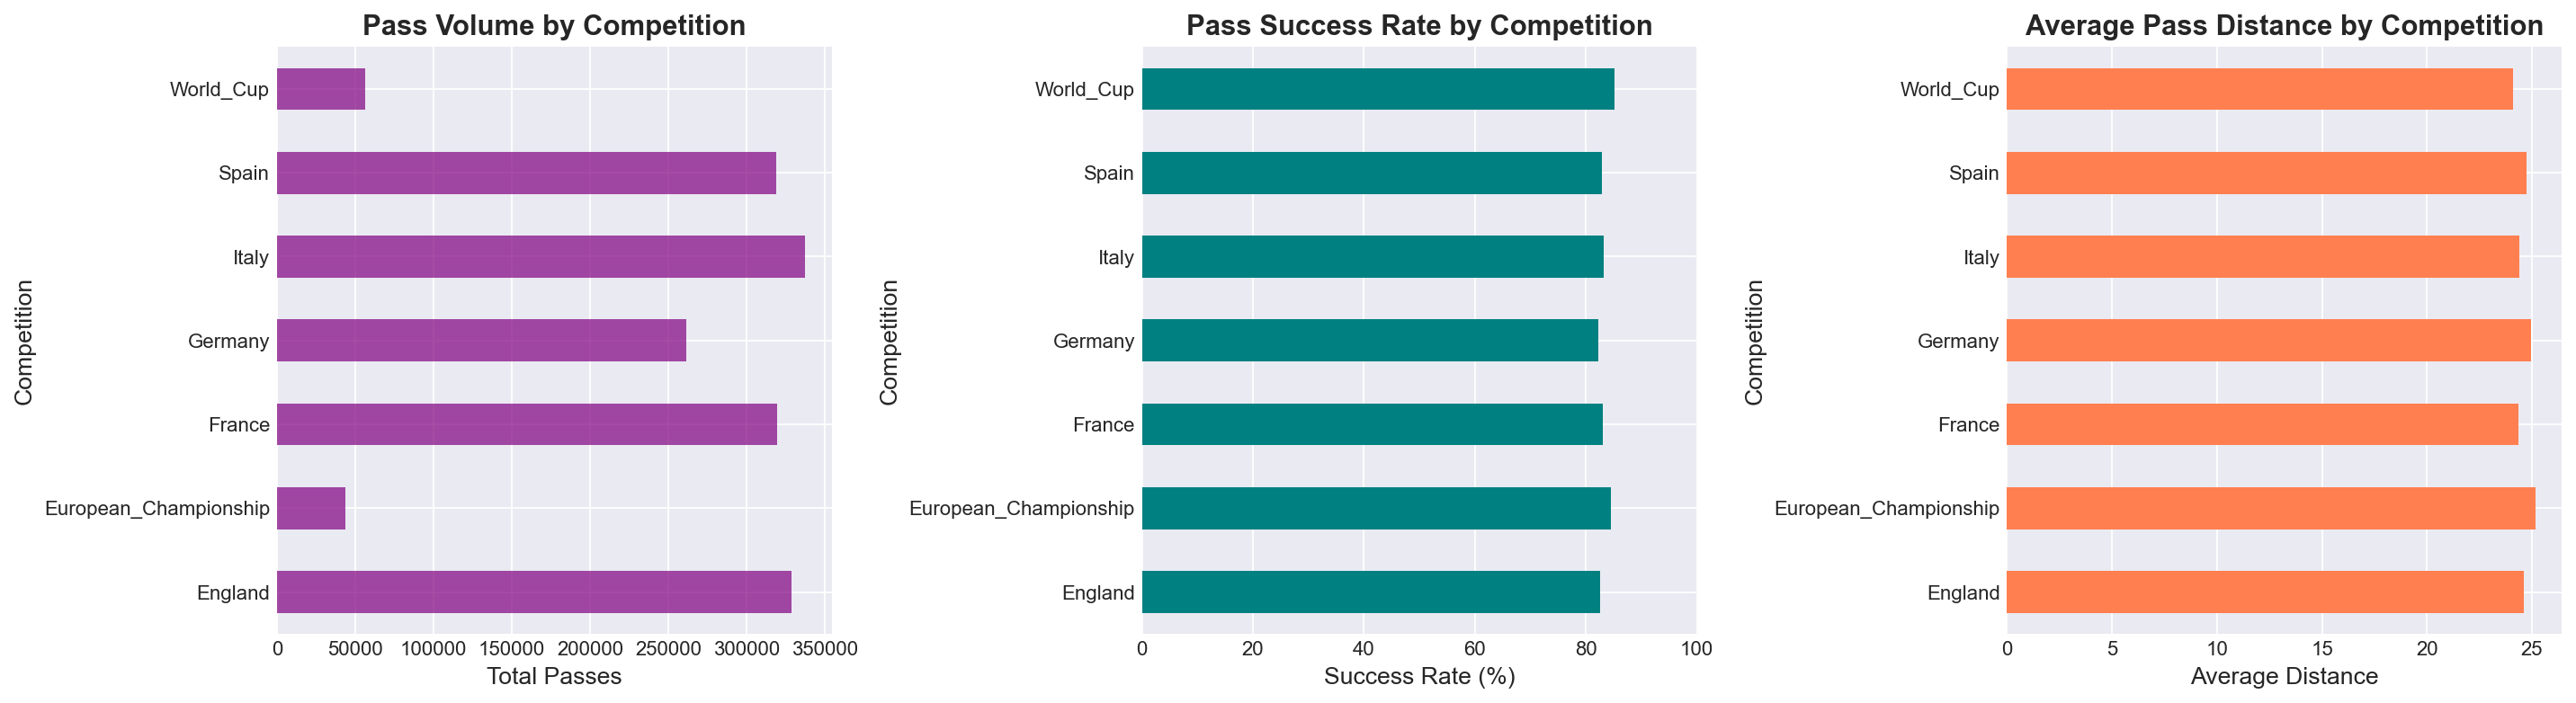
\includegraphics[width=\linewidth]{figures/eda/competition_pass_stats.png}
  \caption{Pass-Statistiken nach Wettbewerb: Volumen, Genauigkeit und durchschnittliche Distanz. Unterschiede deuten auf verschiedene Spielstile und taktische Ansätze hin.}
  \label{fig:competition_pass_stats}
\end{figure}

Auf Basis der vorliegenden Wettbewerbsauswertung liegt die Passgenauigkeit der englischen Liga bei ca. 82.5\% (Abbildung~\ref{fig:competition_pass_stats}), was im professionellen Fussball ein typischer Wert ist (etwa 4 von 5 Pässen kommen an) \parencite{fotmob_no_date}.

\subsection{Erste Hypothesen für die Netzwerk-Analyse}

Basierend auf den EDA-Ergebnissen lassen sich folgende Hypothesen für die nachfolgenden Netzwerkanalysen:

\begin{enumerate}
  \item \textbf{Zentrale Knoten:} Die identifizierten Top-Passgeber werden hohe Degree-Zentralität und Betweenness-Zentralität aufweisen, da sie als Verteiler im Spielaufbau fungieren.
  \item \textbf{Räumliche Cluster:} Die Heatmaps deuten auf räumliche Cluster hin (Abwehr, Mittelfeld, Angriff), die sich in Communitystrukturen der Netzwerke widerspiegeln könnten.
  \item \textbf{Wettbewerbsspezifische Unterschiede:} Ligen mit höherer Pass-Genauigkeit und kürzeren Pässen könnten dichtere Netzwerke mit mehr reziproken Verbindungen aufweisen.
  \item \textbf{Zeitliche Dynamik:} Die beobachteten Aktivitätsmuster über den Spielverlauf legen nahe, dass sich Netzwerkmetriken (z.\,B. Dichte, Zentralisierung) zwischen den Spielphasen unterscheiden.
\end{enumerate}

\section{LE3 -- Netzwerk-Modellierung \& Filterung}

\subsection{Ziel}
Dieses Kapitel dokumentiert die Konstruktion verschiedener Netzwerktypen aus den Fussballdaten sowie die angewandten Filterungstechniken zur Netzwerkreduktion. Basierend auf den Erkenntnissen aus dem EDA erstellen wir vier Netzwerke: Pass-Netzwerke (Spieler--Spieler), Match-Netzwerke (Team--Team), bipartite Spieler--Team-Netzwerke sowie ein Feld-Lokationsnetzwerk (Zone--Zone). Zusätzlich demonstrieren wir die Projektion von Two-Mode-Netzwerken auf One-Mode-Netzwerke und diskutieren die Auswirkungen auf Dichte und Skalierbarkeit.

\subsection{Netzwerkdefinitionen}

\subsubsection{Pass-Netzwerke (Spieler-zu-Spieler)}

\textbf{Netzwerktyp:} Gerichtet, Gewichtet

\textbf{Knoten:} Spieler (eindeutige \texttt{wyId}).

\textbf{Kanten:} Gerichtete Kanten von Passgebern zu Passempfängern. Eine Kante $(u, v)$ existiert, wenn Spieler $u$ erfolgreich einen Pass zu Spieler $v$ gespielt hat.

\textbf{Wesentliche Attribute:} Kanten werden primär über \texttt{pass\_count} (Gewicht) beschrieben. Ergänzend speichern wir (wo sinnvoll) aggregierte Kantenstatistiken wie Distanz und Winkel.

\textbf{Konstruktionsmethode:}
Die Identifikation des Passempfängers erfolgt über ein Matching auf der Eventsequenz. Für jeden erfolgreichen Pass wird der Empfänger als der Spieler identifiziert, der
\begin{itemize}
  \item im selben Team spielt,
  \item nicht der Passgeber ist,
  \item die nächste Aktion innerhalb eines Distanzschwellenwerts von 5 Metern zum Passendpunkt ausführt,
  \item und diese Aktion innerhalb eines Zeitschwellenwerts von 5 Sekunden nach dem Pass ausführt.
\end{itemize}

Die Heuristik ist relativ Robust, sie kann aber bei sehr schnellen Sequenzen oder quasi simultanen Aktionen Fehlzuordnungen verursachen und nicht immer garantieren, einen Empfänger ausfindig zu machen.

\subsubsection{Match-Netzwerke (Team-zu-Team)}

\textbf{Netzwerktyp:} Gerichtet, Gewichtet

\textbf{Knoten:} Fussballteams

\textbf{Kanten:} Gerichtete Kanten zwischen Teams basierend auf Spielergebnissen. Eine Kante $(A, B)$ repräsentiert Spiele, in denen Team $A$ gegen Team $B$ angetreten ist.

\textbf{Kantenattribute:}
\begin{itemize}
  \item \texttt{weight}: Gesamtanzahl der Tore von Team $A$ gegen Team $B$
  \item \texttt{matches}: Anzahl gespielter Spiele
  \item \texttt{wins}, \texttt{losses}, \texttt{draws}: Anzahl Siege, Niederlagen, Unentschieden
  \item \texttt{weight\_normalized}: Durchschnittliche Tore pro Spiel
\end{itemize}

\textbf{Knotenattribute:}
Zentrale Teamattribute sind u.a. \texttt{total\_matches}, aggregierte Resultate (\texttt{wins/losses/draws}) sowie die Torbilanz inkl. \texttt{goal\_difference}.

\textbf{Konstruktionsmethode:}

Das Netzwerk wird direkt aus den Match-Daten konstruiert. Für jedes gespielte Spiel zwischen Team $A$ und Team $B$ mit Ergebnis $s_A : s_B$ werden zwei gerichtete Kanten erstellt:
\begin{itemize}
  \item Kante $(A, B)$ mit Gewicht $s_A$ (Tore von $A$)
  \item Kante $(B, A)$ mit Gewicht $s_B$ (Tore von $B$)
\end{itemize}

Falls mehrere Spiele zwischen denselben Teams stattfinden, werden die Gewichte aggregiert.

\subsubsection{Spieler-Team-Netzwerke (Bipartit / Two-Mode)}

\textbf{Netzwerktyp:} Ungerichtet, Gewichtet, Bipartit

\textbf{Knotenmengen:}
\begin{itemize}
  \item Menge $P$: Spieler
  \item Menge $T$: Teams
\end{itemize}

\textbf{Kanten:} Ungerichtete Kanten zwischen Spielern und \emph{den Teams, für die sie in einem Match gespielt haben}. 

\textbf{Wichtig:} Spieler sind typischerweise nur mit \textbf{einem} Team verbunden; nur bei Teamwechseln innerhalb der Saison treten \textbf{zwei} Teamverknüpfungen auf.

\textbf{Kantenattribute:}
\begin{itemize}
  \item \texttt{matches\_together}: Anzahl der Spiele, in denen der Spieler für dieses Team im Datensatz auflief
  \item \texttt{weight}: Identisch mit \texttt{matches\_together}
\end{itemize}

\textbf{Knotenattribute:}
\begin{itemize}
  \item \texttt{type}: "player" oder "team"
  \item \texttt{bipartite}: 0 für Spieler, 1 für Teams (NetworkX-Konvention)
  \item Spieler-spezifisch: \texttt{name}, \texttt{role}, \texttt{area}, \texttt{teams\_count}
  \item Team-spezifisch: \texttt{team\_name}, \texttt{area}, \texttt{players\_count}
\end{itemize}

\textbf{Konstruktionsmethode:}

Aus den Event-Daten erfassen wir pro Match die Spieler-ID und die zugehörige Team-ID (Team des Events) und aggregieren diese über Match-IDs. Dadurch entsteht pro Spieler typischerweise genau eine Teamkante (bei Transfers zwei), deren Gewicht die Einsatzhäufigkeit approximiert.


\subsubsection{Feld-Netzwerke}

\subsection{Two-Mode zu One-Mode Projektion}
\section{LE3 -- Netzwerk-Modellierung \& Filterung}

\subsection{Netzwerkmodellierung}

\subsubsection{Netzwerke (\,4 Typen\,)}
Wir modellieren vier Netzwerktopologien, die unterschiedliche Aspekte des Spielgeschehens abdecken. Standardformeln werden hier bewusst weggelassen; im Fokus stehen die konkrete Konstruktion und die daraus resultierenden Strukturen.

\paragraph{Pass-Netzwerk (Spieler--Spieler)}
	extbf{Typ:} gerichtet, gewichtet. 
	extbf{Knoten:} Spieler (\texttt{wyId}).
	extbf{Kanten:} gerichtete Kante $(u, v)$, wenn Spieler $u$ einen erfolgreichen Pass zu Spieler $v$ spielt. Hauptgewicht ist \texttt{pass\_count}.

	extbf{Passempfänger (projektspezifisch):} Wyscout liefert nicht in jedem Fall einen expliziten Passempfänger. Wir bestimmen ihn daher über ein raum-zeitliches Matching: zur Pass-Endposition suchen wir im selben Team die nächste Aktion innerhalb von 5 Sekunden und 5 Metern. Der nächstgelegene Kandidat wird als Empfänger gewählt.

\paragraph{Match-Netzwerk (Team--Team)}
	extbf{Typ:} gerichtet, gewichtet.
	extbf{Knoten:} Teams.
	extbf{Kanten:} je Spiel erzeugen wir zwei gerichtete Kanten $(A\rightarrow B)$ und $(B\rightarrow A)$; das Kantengewicht entspricht den erzielten Toren (Aggregationen über mehrere Spiele werden summiert).

\paragraph{Spieler--Team-Netzwerk (Two-Mode)}
	extbf{Typ:} bipartit, ungerichtet, gewichtet.
	extbf{Knoten:} Spieler $P$ und Teams $T$.
	extbf{Kanten:} Kante $(p, t)$, wenn Spieler $p$ in einem Match für Team $t$ auflief; Gewicht \texttt{matches\_together} zählt Einsätze/Match-Beteiligungen.

	extbf{Wichtig:} Spieler sind typischerweise mit genau \textbf{einem} Team verbunden; zwei Teams treten praktisch nur bei Teamwechseln innerhalb der Saison auf.

\subparagraph{Flattening: Projektion auf Spieler (One-Mode)}
Wir projizieren das bipartite Spieler--Team-Netz auf die Spielermenge: zwei Spieler sind verbunden, wenn sie mindestens ein Team teilen; das Kantengewicht steigt mit der Anzahl gemeinsamer Einsätze (bzw. mit den bipartiten Kantengewichten). Dadurch entsteht ein dichteres Spieler--Spieler-Netz, das implizite Teambeziehungen sichtbar macht.

\paragraph{Feld-Lokationsnetzwerk (Zone--Zone)}
	extbf{Typ:} gerichtet, Multi-Edge.
	extbf{Knoten:} diskrete Feldzonen (5$\times$5m Raster, Wyscout-Koordinaten 0--100).
	extbf{Kanten:} Ereignisübergänge von Start- zu Endzone für Pass (8), Schuss (10) und Standards (3). Dieses Netz dient als räumliche Perspektive auf Spielmuster.

\subsubsection{Visualisierung}
Zur Illustration der Modellierung zeigen wir je Netztyp eine Abbildung; für das Player--Team-Netz zusätzlich die Darstellung vor und nach dem Flattening.

\begin{figure}[htbp]
  \centering
  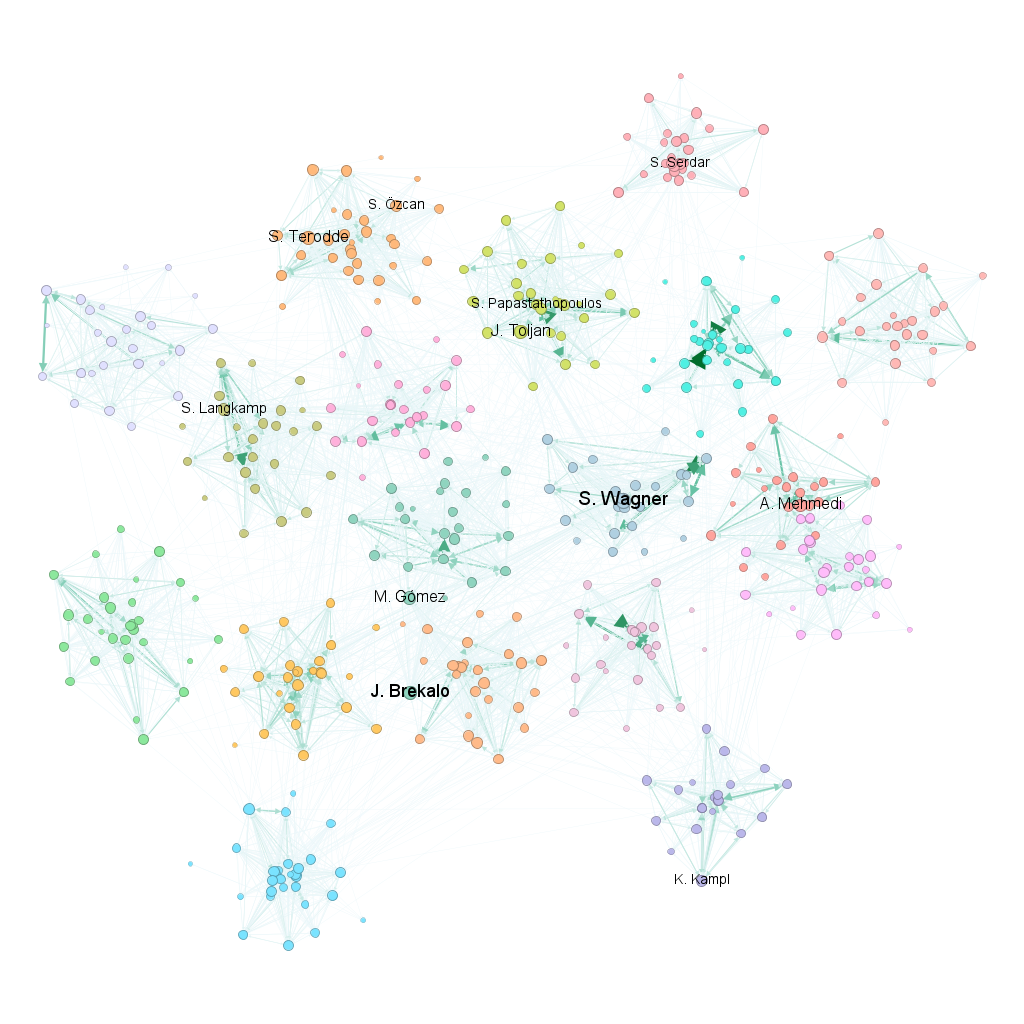
\includegraphics[width=0.9\linewidth,height=0.38\textheight,keepaspectratio]{figures/LE3/pass_network_full.png}
  \caption{Pass-Netzwerk (Beispiel). Knoten = Spieler, gerichtete Kanten = erfolgreiche Pässe, Breite typischerweise proportional zu \texttt{pass\_count}.}
  \label{fig:le3_pass_network_full}
\end{figure}

\begin{figure}[htbp]
  \centering
  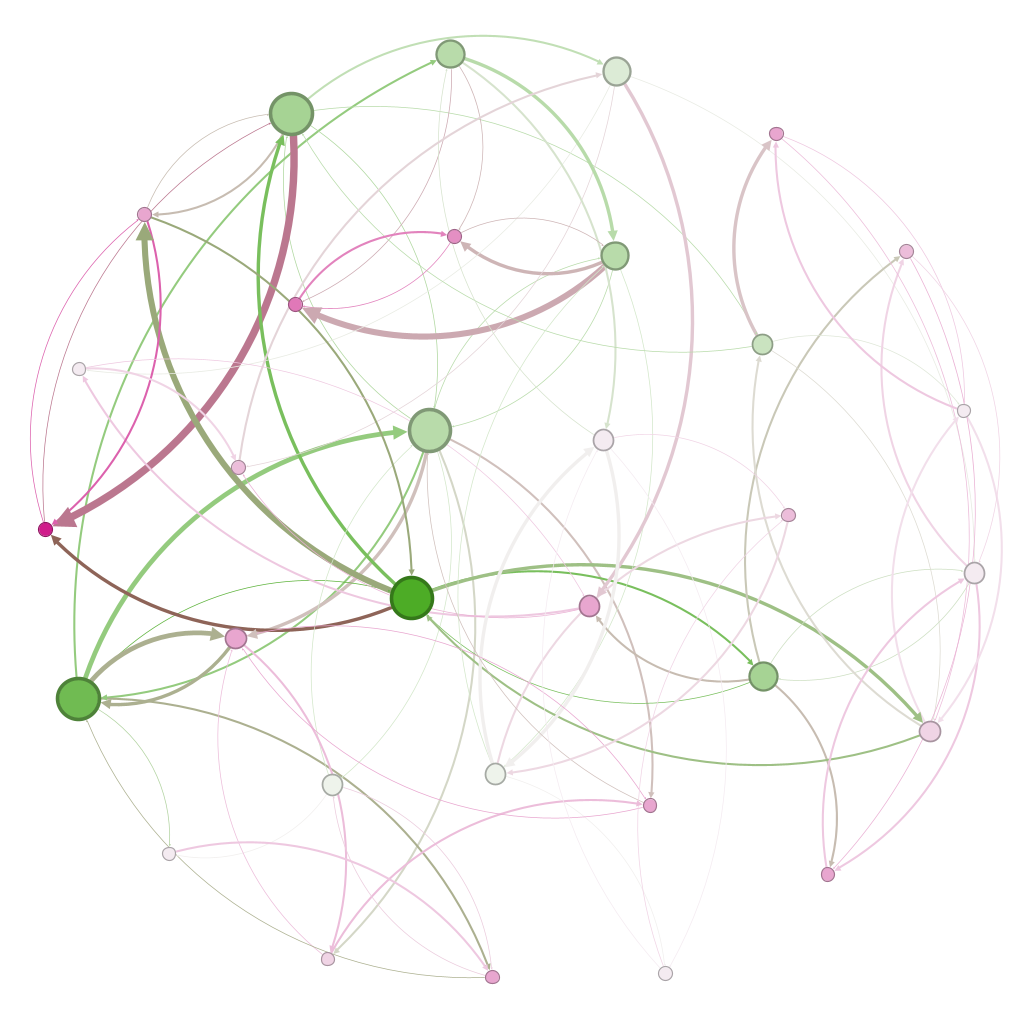
\includegraphics[width=0.9\linewidth,height=0.38\textheight,keepaspectratio]{figures/LE3/match_network_circular.png}
  \caption{Match-Netzwerk (Beispiel). Knoten = Teams, gerichtete Kanten = aggregierte Resultate zwischen Team-Paaren.}
  \label{fig:le3_match_circular}
\end{figure}

\begin{figure}[htbp]
  \centering
  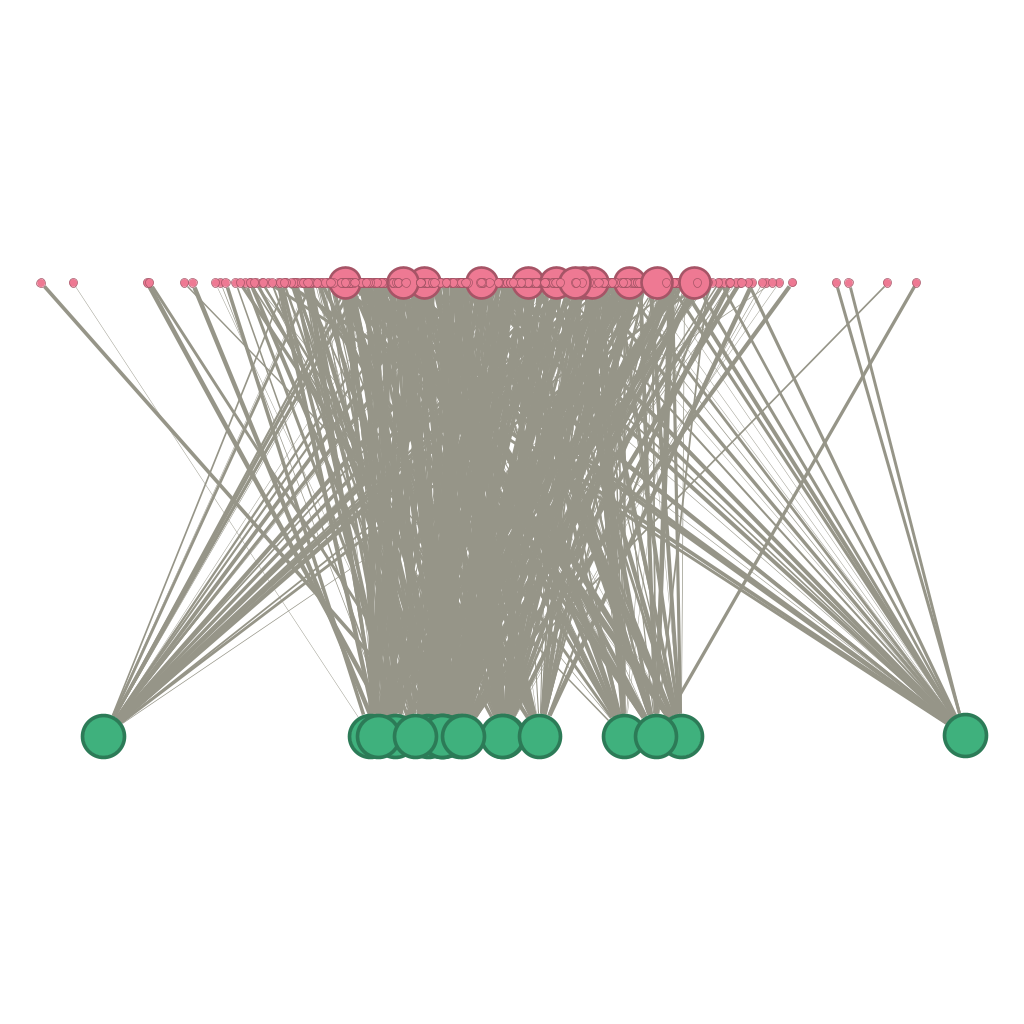
\includegraphics[width=0.9\linewidth,height=0.38\textheight,keepaspectratio]{figures/LE3/bipartite_network.png}
  \caption{Player--Team Two-Mode Netzwerk (vor Flattening). Spieler sind typischerweise genau einem Team zugeordnet (zwei bei Teamwechsel); Kantenbreite kodiert \texttt{matches\_together}.}
  \label{fig:le3_player_team_before}
\end{figure}

\begin{figure}[htbp]
  \centering
  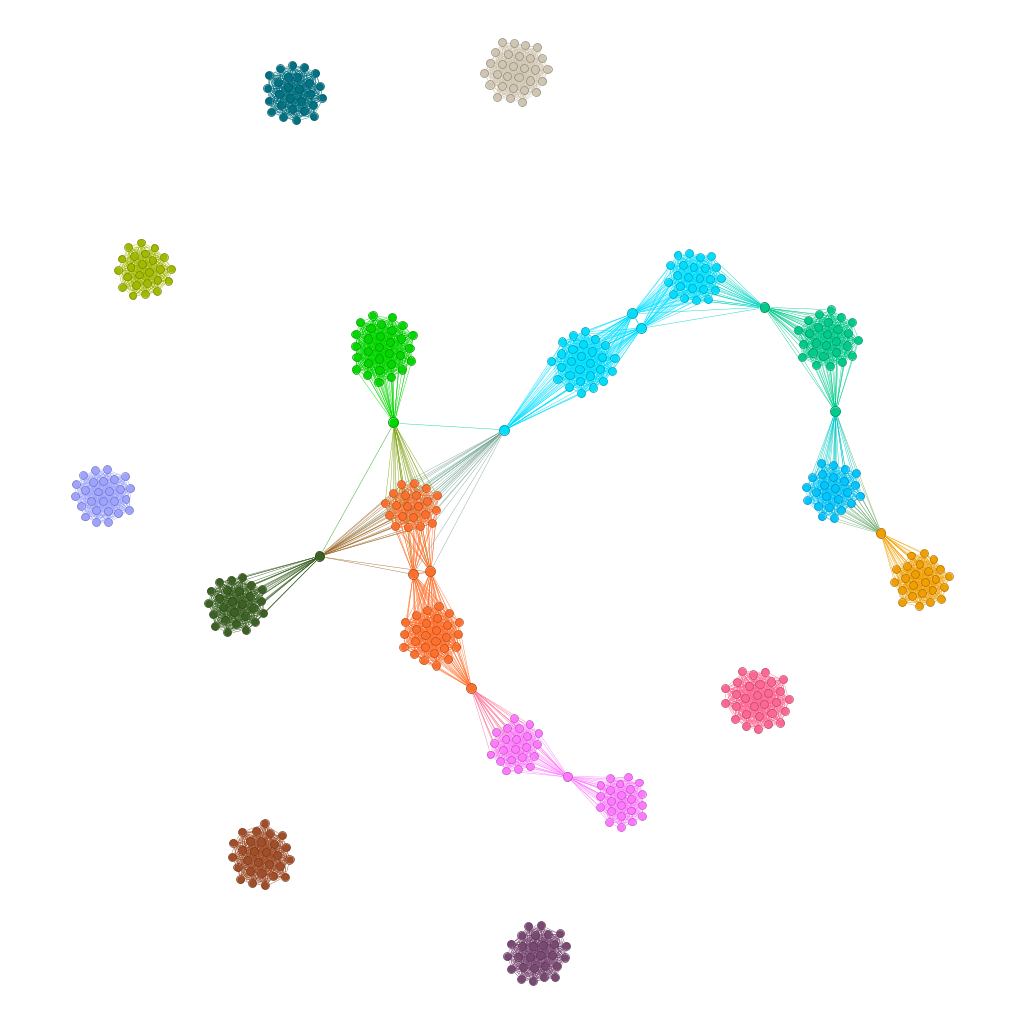
\includegraphics[width=0.9\linewidth,height=0.38\textheight,keepaspectratio]{figures/LE3/player_projection_network.png}
  \caption{Player--Player Netzwerk (nach Flattening / Projektion). Eine Kante entsteht durch gemeinsames Team; Gewichte akkumulieren gemeinsame Einsätze.}
  \label{fig:le3_player_team_after}
\end{figure}

\begin{figure}[htbp]
  \centering
  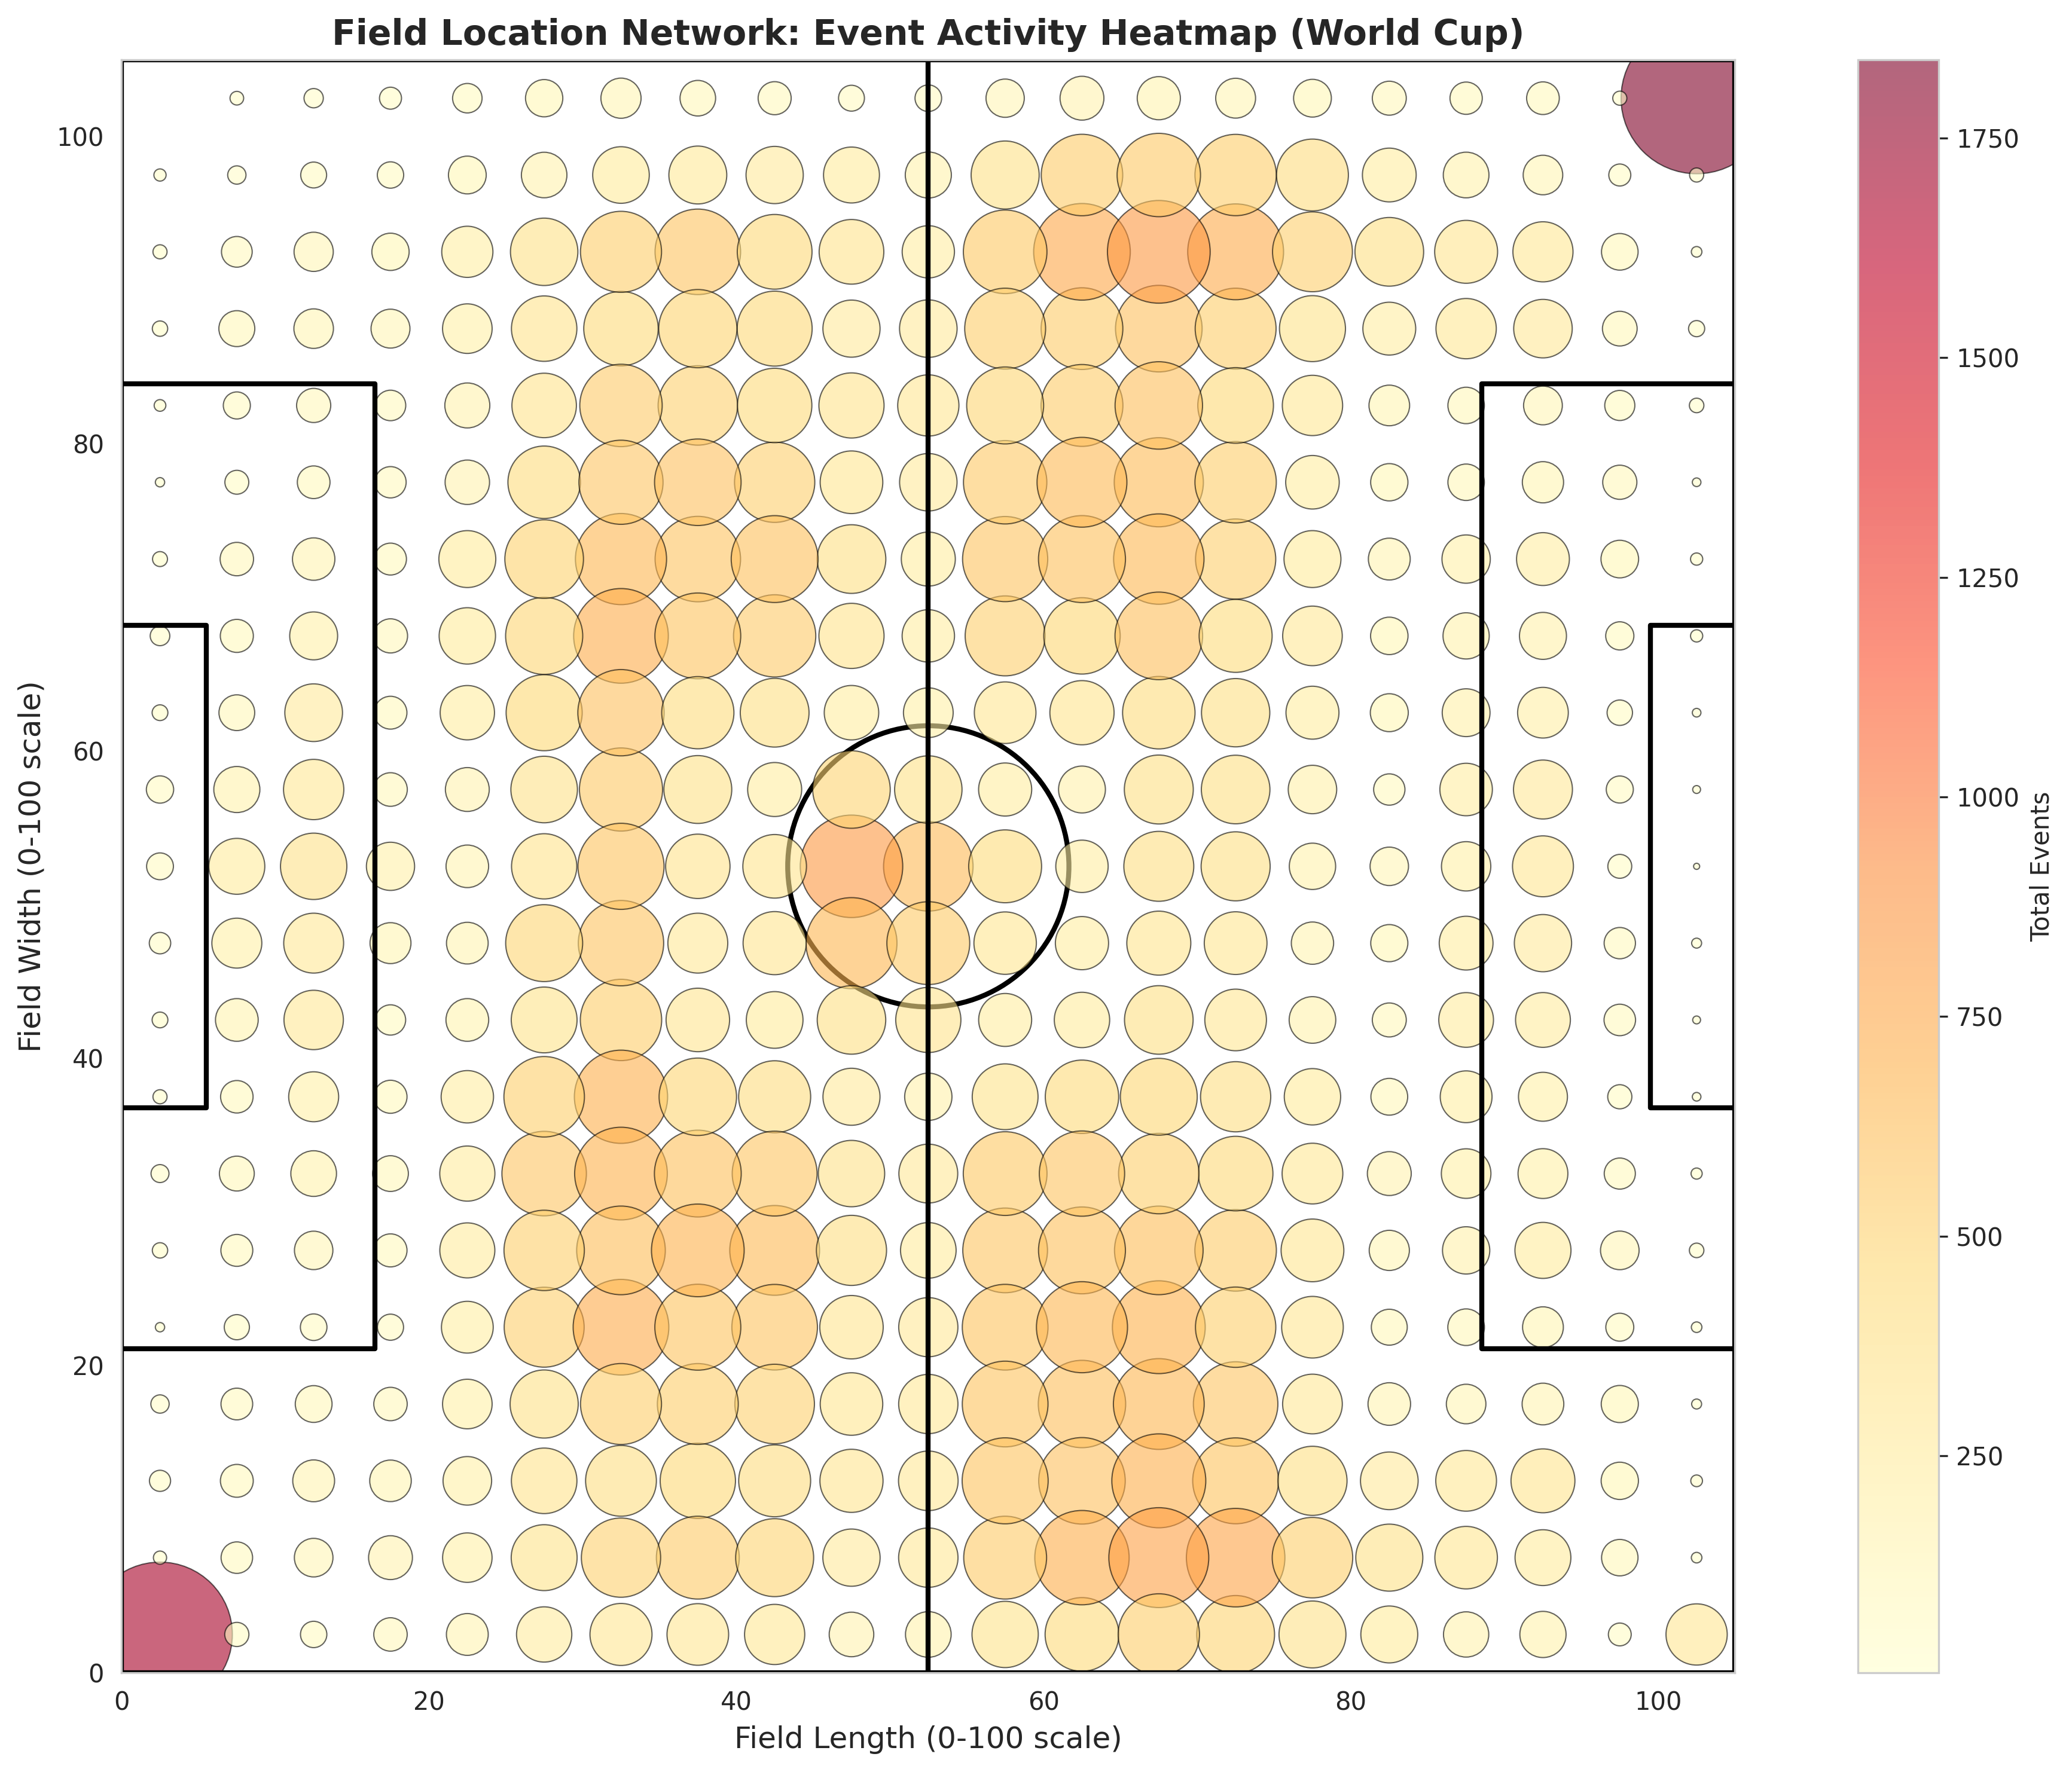
\includegraphics[width=0.9\linewidth,height=0.38\textheight,keepaspectratio]{figures/LE3/field_network_heatmap.png}
  \caption{Feld-Lokationsnetzwerk (Beispiel) als Heatmap. Farbe/Grösse kodieren Ereignisintensität in diskreten Feldzonen.}
  \label{fig:le3_field_heatmap}
\end{figure}

\subsection{Netzwerkfilterung}

In diesem Kapitel beschreiben wir, wie wir Filterung und Sichten (Local/Global/Ego) einsetzen, um aus grossen Netzwerken analysierbare Teilstrukturen zu extrahieren. Der Fokus liegt auf der praktischen Nutzung: welche Fragen lassen sich damit beantworten, und welche Visualisierungen stützen die Interpretation.

\subsubsection{Sichten: Local View, Global View, Ego-Netzwerk}

\paragraph{Local View (z.B. nur ein Team)}
Eine lokale Sicht extrahiert typischerweise ein Team-Subgraph aus dem Pass-Netzwerk (nur Pässe zwischen Spielern desselben Teams). Damit kann man z.B. untersuchen, ob die Stärke und Zentralisierung der teaminternen Verknüpfungen mit sportlichem Erfolg korrelieren (z.B. Punkte, Tore, Goal Difference).

\begin{figure}[htbp]
  \centering
  \includegraphics[width=0.9\linewidth,height=0.36\textheight,keepaspectratio]{figures/LE3/local_view_team_placeholder.png}
  \caption{\textbf{Platzhalter:} Local View eines Team-Subgraphs im Pass-Netzwerk (bitte passende Abbildung exportieren/benennen).}
  \label{fig:le3_local_view_team}
\end{figure}

\paragraph{Global View (z.B. Wettbewerb/League als Ganzes)}
Die globale Sicht betrachtet das komplette Netzwerk eines Wettbewerbs (z.B. gesamtes Match-Netz oder gesamtes Pass-Netz pro Competition). Sie dient dem Vergleich zwischen Competitions oder zur Einordnung von Extremwerten (z.B. Dichte, Komponenten, Gradverteilungen).

\begin{table}[h]
\centering
\caption{übersicht der konstruierten Netzwerke (Germany; aus \texttt{.gexf} berechnet)}
\label{tab:network_summary}
\begin{tabular}{lcccc}
	oprule
	extbf{Netzwerktyp} & \textbf{|V|} & \textbf{|E|} & \textbf{Dichte} & \textbf{Komponenten} \\
\midrule
Pass-Netzwerk & 473 & 8786 & 0.039354 & 8 \\
Match-Netzwerk & 18 & 306 & 1.000000 & 1 \\
Spieler-Team-Netzwerk & 492 & 503 & 0.004164 & 1 \\
Spieler-Projektion & 474 & 6803 & 0.060686 & 1 \\
\bottomrule
\end{tabular}
\end{table}

\begin{figure}[htbp]
  \centering
  \includegraphics[width=0.9\linewidth,height=0.36\textheight,keepaspectratio]{figures/LE3/global_view_placeholder.png}
  \caption{\textbf{Platzhalter:} Global View (z.B. Gesamtgraph eines Wettbewerbs, oder Vergleich mehrerer Competitions in einer Grafik).}
  \label{fig:le3_global_view}
\end{figure}

\paragraph{Ego-Netzwerk (Spielerfokus)}
Ego-Netzwerke isolieren die unmittelbare Umgebung eines Spielers (Ego) und sind hilfreich, um Rollen im Teamkontext zu interpretieren (z.B. als Connector/Hub) oder konkrete Passpartner-Strukturen zu visualisieren.

\begin{figure}[htbp]
  \centering
  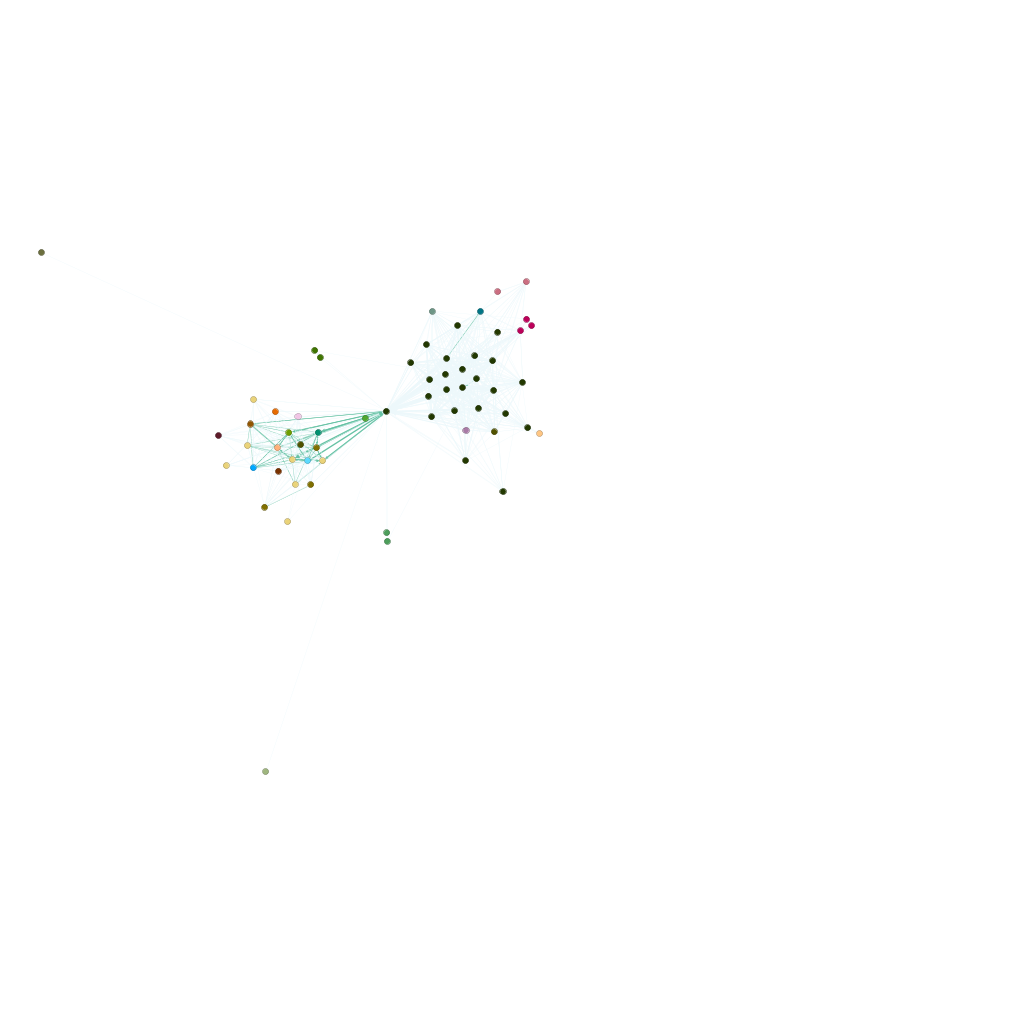
\includegraphics[width=0.9\linewidth,height=0.36\textheight,keepaspectratio]{figures/LE3/Ego_granitXhaka.png}
  \caption{Ego-Netzwerk von Granit Xhaka (\textbf{Platzhalter falls Datei noch fehlt:} bitte unter \texttt{figures/LE3/Ego\_granitXhaka.png} ablegen).}
  \label{fig:le3_ego_xhaka}
\end{figure}

\subsubsection{Filtern anhand von Kantenattributen}
Wir setzen Kantenattribut-Filter ein, um "Rauschen" zu reduzieren und stabilere Beziehungen hervorzuheben. Im Pass-Netzwerk ist das zentrale Filterkriterium typischerweise \texttt{pass\_count} (Mindestanzahl Pässe pro Kante); optional sind Filter nach Genauigkeit oder Distanz sinnvoll.

Für Germany zeigt die gewichtsbasierte Filterung (nach Entfernen isolierter Knoten) z.B.:
\begin{itemize}
  \item $w \geq 5$: 91.1\% Knoten, 71.9\% Kanten erhalten
  \item $w \geq 10$: 85.6\% Knoten, 56.2\% Kanten erhalten
  \item $w \geq 20$: 76.7\% Knoten, 36.8\% Kanten erhalten
\end{itemize}

\begin{figure}[htbp]
  \centering
  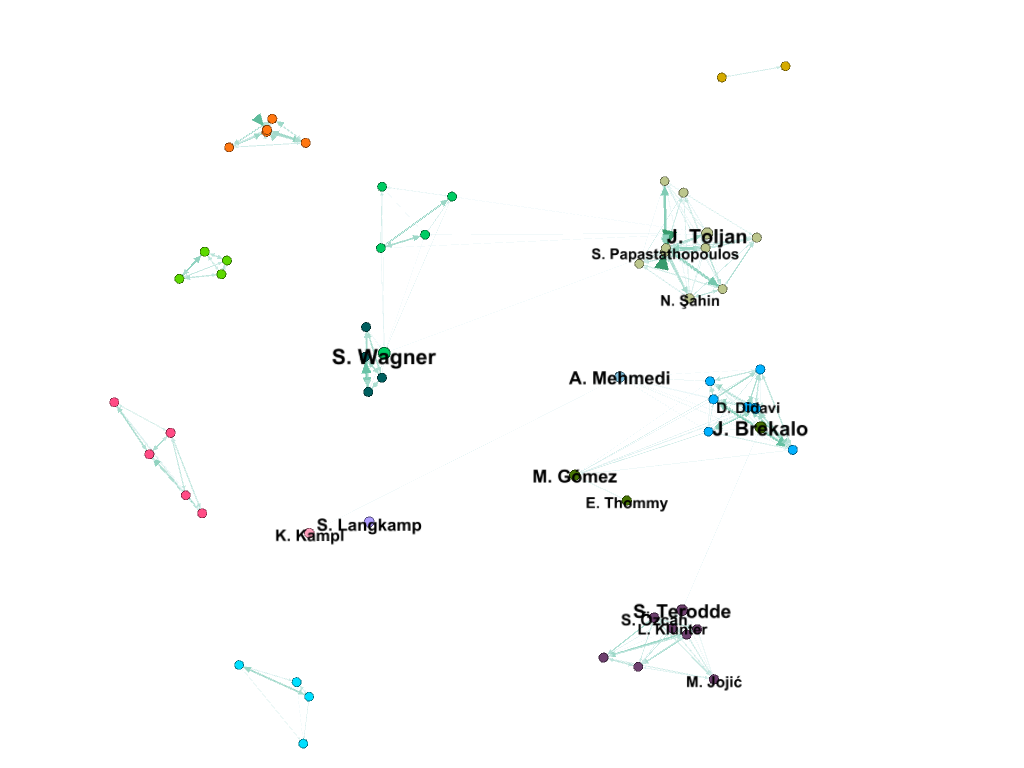
\includegraphics[width=0.9\linewidth,height=0.36\textheight,keepaspectratio]{figures/LE3/pass_network_filtered.png}
  \caption{Filterung nach Kantenattribut (Beispiel). \textbf{Falls diese Abbildung nicht die Filterkurve zeigt:} bitte eine passende Visualisierung exportieren und den Dateinamen hier anpassen.}
  \label{fig:le3_edge_attr_filter}
\end{figure}

\subsubsection{Offene Visualisierungen (benötigte Exporte)}
Wenn du willst, kann ich die Platzhalter direkt auf konkrete Dateinamen/Abbildungsunterschriften anpassen. Aktuell fehlen im Repo nur die Grafiken für:
\begin{itemize}
  \item Local View eines konkreten Teams (Pass-Subgraph)
  \item Global View (z.B. Competition-Vergleich oder Gesamtgraph als Plot)
\end{itemize}
Sag mir einfach, welche Competition/Teams du zeigen möchtest (und ob du eher Gephi-Viz oder Matplotlib/Seaborn-Plots bevorzugst).
  \centering

\section{LE4 -- Communities}

In diesem Kapitel untersuchen wir, welche Untergruppen wir in unseren wyscouts Fussball Netzwerken identifizieren können. Wir beschränken uns auf Das Netzwerk für die Bundesliga sowie auf den Worldcup.\\
Wir betrachten drei Aspekte: (1) \textbf{Connected Components} als grundlegende Zusammenhangsstruktur, (2) \textbf{Cliquen} als maximale vollständig vernetzte Gruppen und (3) \textbf{Community Detection} zur Identifikation von dichter verbundenen, aber nicht notwendigerweise vollständig vernetzten Gruppen. 

Im Kontext von Fussball erwarten wir:
\begin{itemize}
  \item \textbf{Pass-Netzwerke}: Teams als Communities; Spielformationen als dichtere Substrukturen
  \item \textbf{Match-Netzwerke}: Turniergruppen
  \item \textbf{Feld-Netzwerke}: Cluster von Verteidigungs und Angrifsfeldern.
\end{itemize}

\subsection{Connected Components}

Connected Components beschreiben die grundlegende Zusammenhangsstruktur eines Netzwerks: Gruppen von Knoten, die über Pfade erreichbar sind, aber untereinander nicht verbunden sind.

\paragraph{Pass-Netzwerk (Deutschland)}
Das Pass-Netzwerk \ref{fig:pass_network_connected} zeigt erwartungsgemäss starke Fragmentierung:
\begin{itemize}
  \item \textbf{8 schwach verbundene Komponenten}: Die grösste enthält 473 Knoten (59.8\% des Netzwerks), die übrigen sind isolierte Spieler oder kleine Gruppen
  \item \textbf{Interpretation}: Die grösste Komponente umfasst Spieler mit mindestens indirekten Passverbindungen. Isolierte Komponenten sind typischerweise Ersatzspieler mit minimalem Einsatz oder Fehler in der Passempfänger-Identifikation
\end{itemize}

\begin{figure}[ht]
  \centering
  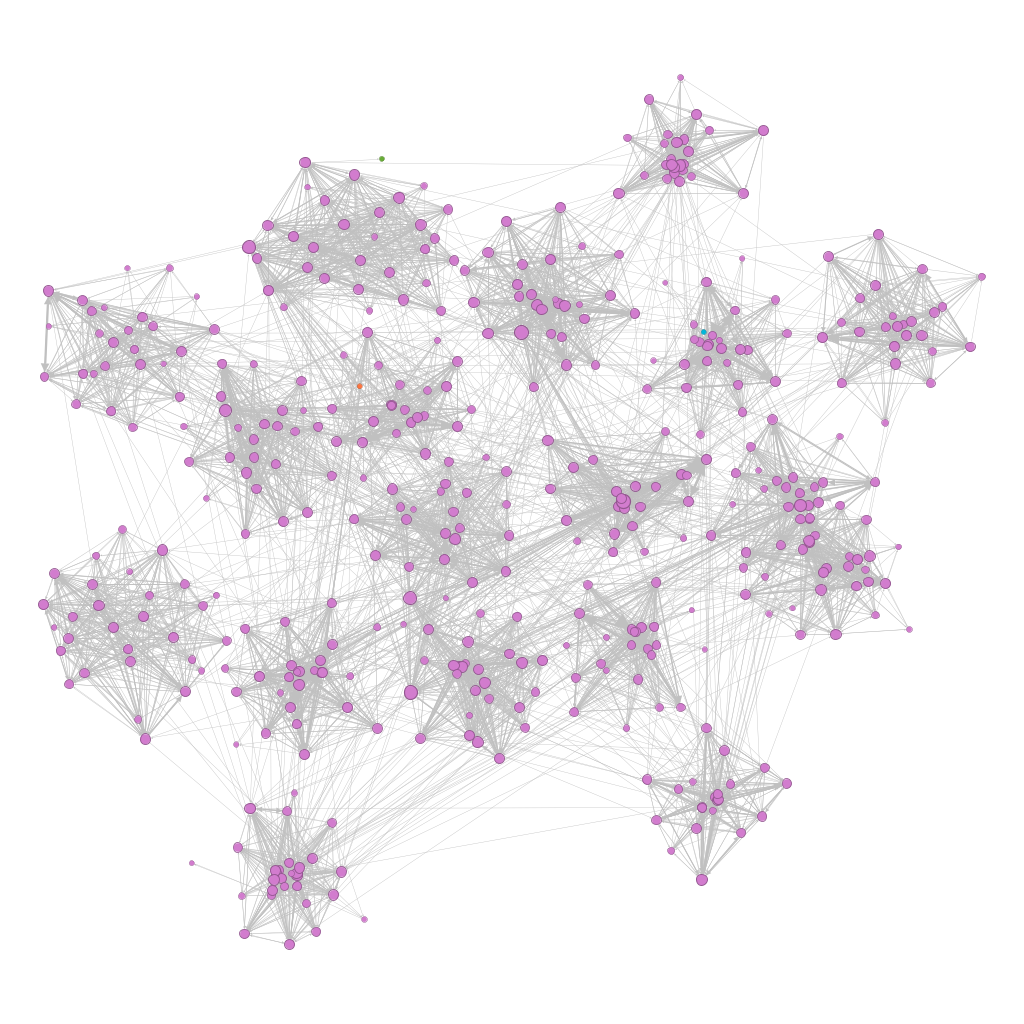
\includegraphics[width=\linewidth]{figures/LE4/pass_network_connected.png}
  \caption{Connected Components im Pass-Netzwerk (Deutschland). Die grösste Komponente umfasst 473 Knoten (59.8\% des Netzwerks), die übrigen sind Teams ohne Transferspieler}
  \label{fig:pass_network_connected}
\end{figure}

\paragraph{Match-Netzwerk (World Cup)}
Match-Netzwerke sind aufgrund der Turnierstruktur typischerweise stark verbunden:
\begin{itemize}
  \item \textbf{1 starke Komponente}: Alle 32 Teams sind über gerichtete Pfade erreichbar
  \item \textbf{Interpretation}: Das Turnier-Format (Gruppenphase + K.O.-Runden) garantiert einen zusammenhängenden Graphen; jedes Team spielt mindestens 3 Spiele
\end{itemize}

\textbf{Praktische Bedeutung}: Für Community Detection verwenden wir primär die grösste zusammenhängende Komponente, da isolierte Knoten keine sinnvollen Community-Zuordnungen erlauben.

\subsection{Cliquen und dichte Subgraphen}

Cliquen sind maximale vollständig vernetzte Untergruppen: jeder Knoten ist mit jedem anderen direkt verbunden. Im Fussball sind echte Cliquen selten (nicht jeder Spieler passt zu jedem), daher betrachten wir auch relaxierte Varianten.

\subsubsection{Maximale Cliquen}

\paragraph{Pass-Netzwerk (Deutschland)}
\textbf{Grösste Cliquen:} 4--5 Knoten (Spieler). Diese entsprechen typischerweise engen Passdreieck/-vierecken innerhalb eines Teams (z.B. Innenverteidiger + zentrales Mittelfeld).

\textbf{Anzahl maximaler Cliquen:} Sehr hoch (Hunderte), da viele lokale, überlappende Passdreiecke existieren. Die meisten haben Grösse 3 (Dreiecke), einige wenige erreichen 4--5.

\paragraph{Match-Netzwerk (World Cup)}
\textbf{Grösste Cliquen:} Bis zu 4 Knoten (Teams). Dies entspricht vollständig vernetzten Vierergruppen in der WM-Vorrunde: jedes Team spielt gegen jedes andere in der Gruppe.

\textbf{Interpretation:} Die Cliquen-Grösse 4 reflektiert direkt die Gruppenstruktur (4 Teams pro Gruppe). K.O.-Spiele erzeugen keine grösseren Cliquen, da nicht alle möglichen Paarungen gespielt werden.

\subsubsection{k-Core Dekomposition}

Der $k$-Core ist der maximale Subgraph, in dem jeder Knoten mindestens Grad $k$ hat. Diese Zerlegung identifiziert zunehmend dichter vernetzte "Kerne" im Netzwerk.

\paragraph{Pass-Netzwerk (Deutschland, grösste Komponente)}
\begin{itemize}
  \item \textbf{Maximaler Core:} $k = 38$ (27 Knoten)
  \item \textbf{Interpretation:} Diese Spieler sind alle vom Verein Köln, was dafür Spricht das sie viel Untereinander passen oder viele Fehlpässe zu anderen Spielern habenTeams
  \item \textbf{Core-Verteilung:} Die meisten Spieler liegen in $k = 22$--$29$, was typischen Team-internen Passmustern entspricht
\end{itemize}

\paragraph{Match-Netzwerk (World Cup)}
\begin{itemize}
  \item \textbf{Maximaler Core:} $k = 4$
  \item \textbf{Interpretation:} Alle Teams sind nur mit ihren Gruppe gut verknüpft.
\end{itemize}

\textbf{Vergleich zu Cliquen:} Während Cliquen vollständige Vernetzung fordern, erlaubt der $k$-Core Flexibilität: Knoten müssen nur mindestens $k$ Verbindungen haben, nicht zu allen anderen.

\subsection{Community Detection}

Community Detection identifiziert Gruppen mit hoher interner und niedriger externer Vernetzung. Anders als Cliquen müssen Communities nicht vollständig vernetzt sein. Wir vergleichen vier Algorithmen: Louvain Algorythmus, Labelpropagation, Fast-Greedy (Clauset-Newman-Moore, \cite{Clauset_2004}) sowie Edge-Betweenes (Girvan-Newman).

\subsubsection{Algorithmen im Überblick}

\paragraph{1. Louvain-Methode}
Ein hierarchischer, gieriger Algorithmus zur \textbf{Maximierung der Modularität}.

\textbf{Laufzeit:} typischerweise $O(m)$ bis $O(n \log n)$ (implementations- und datenabhängig).

\begin{itemize}
  \item Gut skalierbar
  \item Resultate können je nach Implementierung leicht variieren 
  \item Liefert eine hierarchische Community-Struktur
\end{itemize}

\paragraph{2. Label Propagation}
Ein iterativer Algorithmus, bei dem Knoten das häufigste Nachbarschaftslabel übernehmen, bis Konvergenz erreicht ist.

\textbf{Laufzeit:} typischerweise $O(m)$ pro Durchlauf; Gesamtaufwand abhängig von der Anzahl Iterationen.

\textbf{Verhalten/Eigenschaften:}
\begin{itemize}
  \item Extrem schnell
  \item häufig nicht-deterministisch
  \item Keine direkte Optimierung einer globalen Zielfunktion.
\end{itemize}

\paragraph{3. Greedy Modularity (Clauset--Newman--Moore)}
Ein agglomeratives Verfahren, das Communities iterativ so zusammenführt, dass die \textbf{Modularität} am stärksten steigt.

\textbf{Laufzeit:} klassisch $O(md \log n)$ (mit $d$ als mittlerem Grad).

\begin{itemize}
  \item Deterministisch bei fixer Tie-Breaking-Strategie.
  \item Liefert ein hierarchisches Merge-Dendrogram.
  \item Gute Qualität auf vielen Netzwerken, aber weniger skalierbar als Louvain bei sehr grossen Graphen
\end{itemize}

\paragraph{4. Girvan--Newman (Edge Betweenness)}
Ein divisiver Algorithmus, der iterativ Kanten mit hoher Edge-Betweenness entfernt und so Communities separiert.

\textbf{Laufzeit:} typischerweise $O(m^2 n)$ (je nach Implementierung/Variante).


\begin{itemize}
  \item Sehr rechenintensiv
  \item Erzeugt ein vollständiges Dendrogram und erlaubt die Wahl eines Schnittniveaus
  \item Vorallem Historisch/konzeptionell wichtig
\end{itemize}

\subsubsection{Modularität als Qualitätsmass}

Modularität $Q$ misst, wie stark die Vernetzung innerhalb von Communities die Erwartung (unter Random-Graph-Annahme) übertrifft. Werte nahe 1 bedeuten starke Community-Struktur; Werte nahe 0 bedeuten zufällige Vernetzung.

\textbf{Technische Anpassungen:}
\begin{itemize}
  \item Da die meisten Algorithmen für ungerichtete Graphen konzipiert sind, konvertieren wir gerichtete Netzwerke, indem wir Gewichte in beiden Richtungen addieren
  \item \textbf{Gewichte:} Alle Algorithmen berücksichtigen Kantengewichte (\texttt{weight='weight'})
\end{itemize}

\subsection{Ergebnisse: Community Detection}

\subsubsection{Pass-Netzwerk (Deutschland Bundesliga)}

Für die Community Detection verwenden wir die grösste zusammenhängende Komponente (283 Knoten, 59.8\% des Netzwerks).

\begin{table}[h]
\centering
\caption{Algorithmenvergleich auf Pass-Netzwerk (Deutschland, grösste Komponente)}
\label{tab:pass_community_results}
\resizebox{\textwidth}{!}{%
\begin{tabular}{lcccccc}
\toprule
\textbf{Algorithmus} & \textbf{Communities} & \textbf{Modularität} & \textbf{Coverage} & \textbf{Min} & \textbf{Max} & \textbf{Ø Grösse} \\
\midrule
Louvain & 11 & 0.886 & 0.941 & 23 & 31 & 25.7 \\
Label Propagation & 10 & 0.879 & 0.955 & 23 & 51 & 28.3 \\
Greedy Modularity & 11 & 0.884 & 0.940 & 23 & 30 & 25.7 \\
Girvan-Newman & 12 & 0.881 & 0.939 & 1 & 30 & 23.6 \\
\bottomrule
\end{tabular}%
}
\end{table}

\textbf{Beobachtungen:}
\begin{itemize}
  \item \textbf{Sehr hohe Modularität} ($Q > 0.88$): Pass-Netzwerke zeigen extrem starke Community-Struktur -- Spieler passen primär zu Teamkollegen
  \item \textbf{Konsistenz:} Alle Algorithmen finden 10--12 Communities mit ähnlichen Grössen (23--31 Spieler)
  \item \textbf{Hohe Coverage} ($> 0.94$): Über 94\% der Pässe erfolgen innerhalb von Communities
  \item \textbf{Louvain empfohlen:} Höchste Modularität, deterministisch, schnell
\end{itemize}

Abbildung~\ref{fig:pass_communities_algorithm_comparison} zeigt den direkten Vergleich der Algorithmen: Modularität, Anzahl Communities und Grössenverteilungen sind sehr ähnlich, was die Robustheit der gefundenen Struktur bestätigt.

\begin{figure}[h]
  \centering
  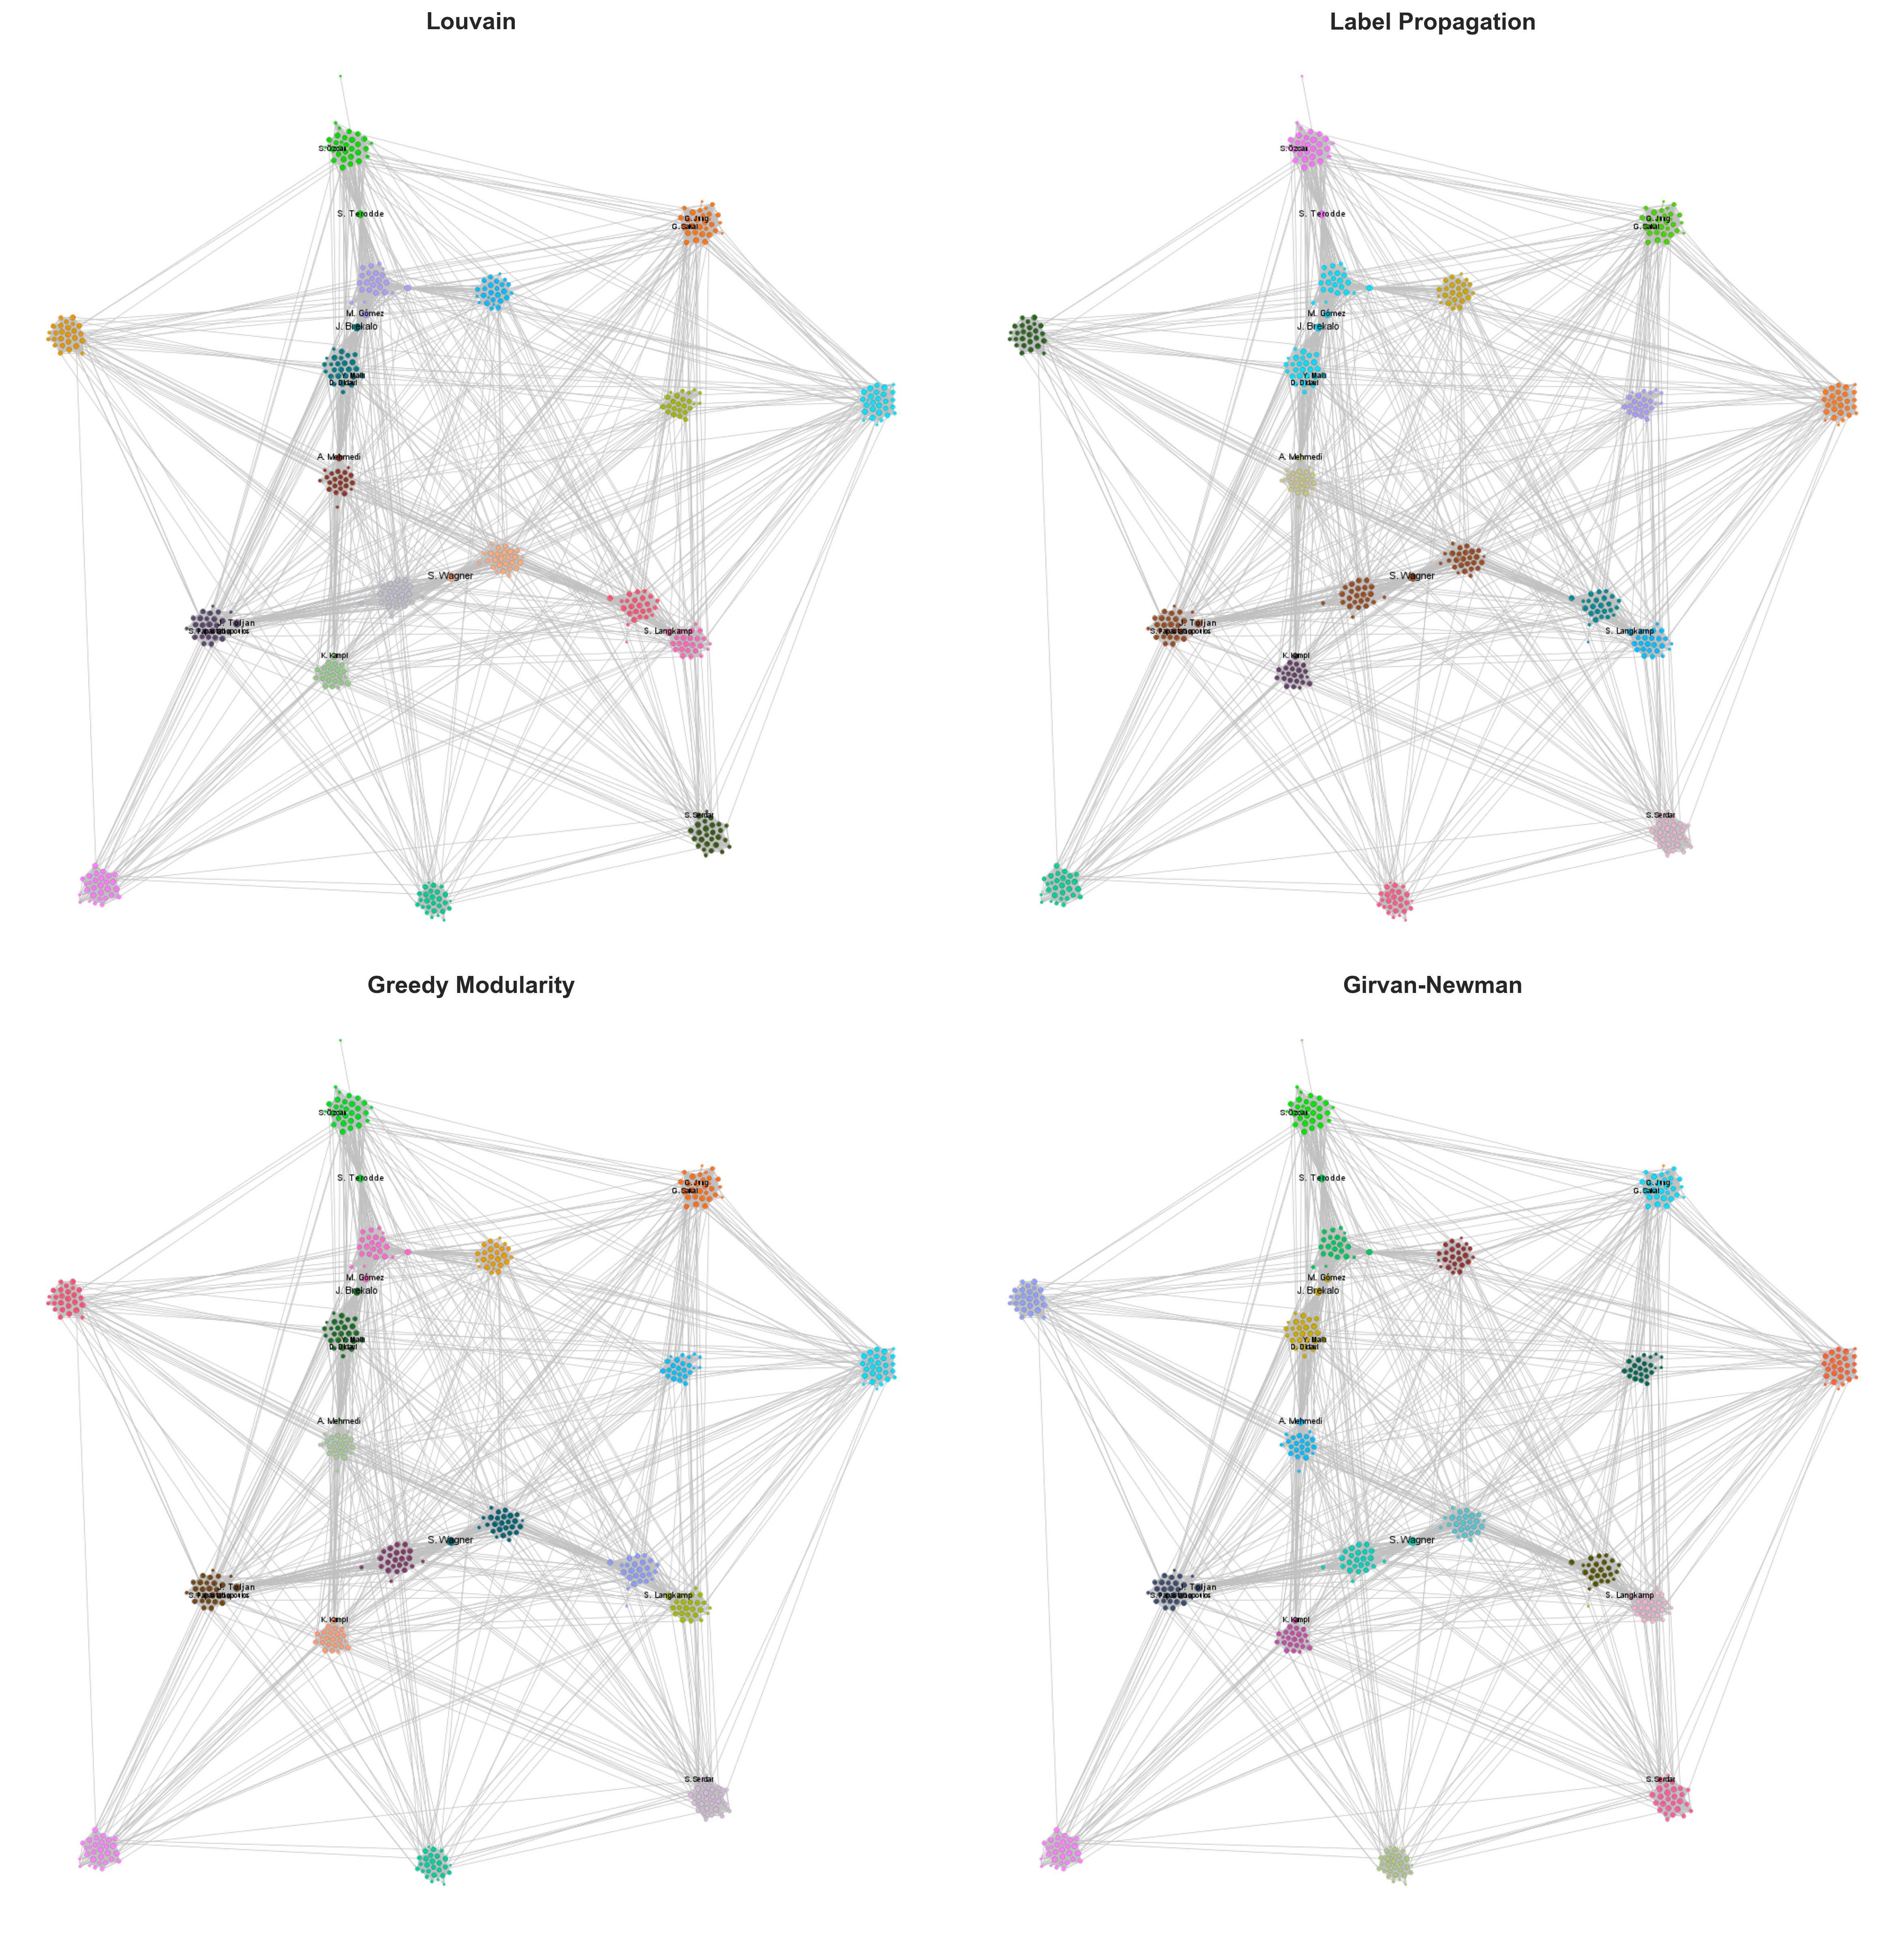
\includegraphics[width=\linewidth]{figures/LE4/pass_communities_algorithm_comparison.png}
  \caption{Algorithmenvergleich auf dem Pass-Netzwerk (Deutschland). Louvain erzielt die höchste Modularität ($Q = 0.886$), Label Propagation die höchste Coverage aber mit einer sehr grossen Ausreisser-Community (Max 51).}
  \label{fig:pass_communities_algorithm_comparison}
\end{figure}

\begin{figure}[h]
  \centering
  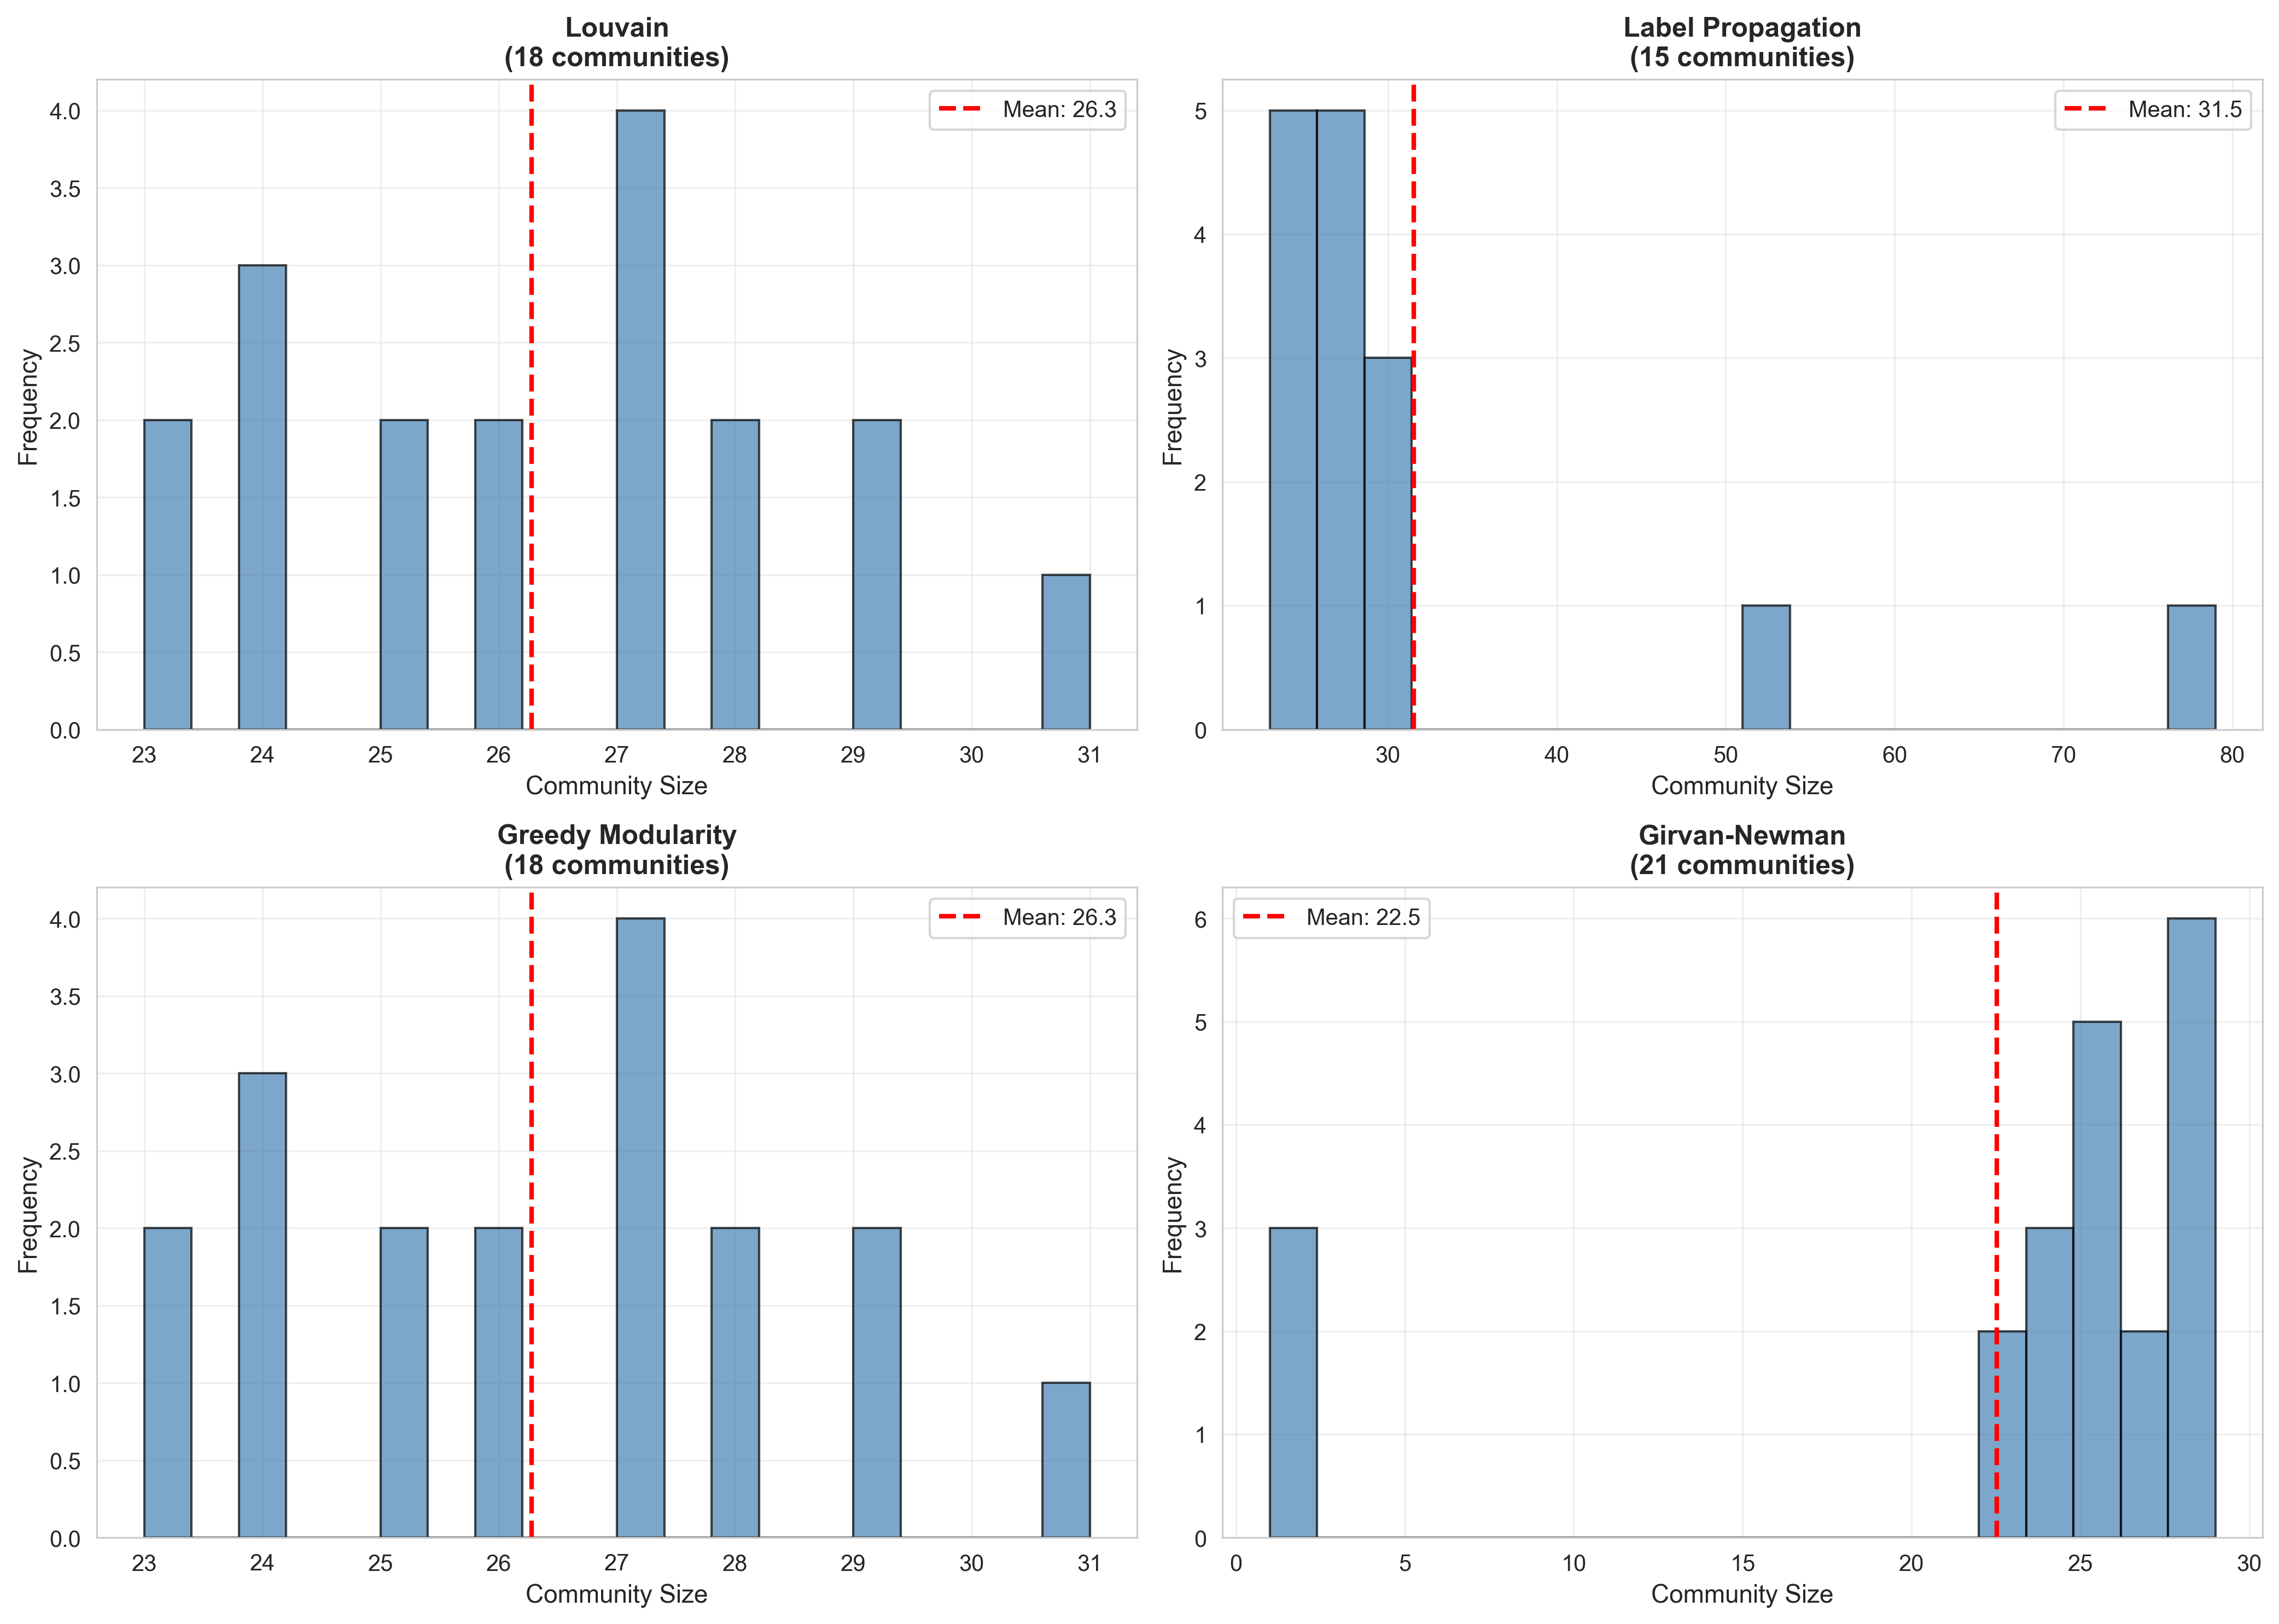
\includegraphics[width=0.95\linewidth]{figures/LE4/pass_communities_louvain.png}
  \caption{Grössenverteilungen der Communities für vier Algorithmen. Louvain und Greedy liefern sehr uniforme Grössen (23--31), Label Propagation zeigt einen Ausreisser (bis 51), Girvan-Newman produziert eine Singleton-Community.}
  \label{fig:community_size_dist}
\end{figure}

\paragraph{Interpretation: Communities = Teams}
Die algorithmisch gefundenen Communities entsprechen nahezu perfekt den realen Teams. Analyse der Louvain-Communities zeigt:
\begin{itemize}
  \item Community 1 (31 Spieler): 100\% FC Köln
  \item Community 2 (28 Spieler): 100\% Borussia Dortmund  
  \item Community 3 (27 Spieler): 96.3\% VfL Wolfsburg, 3.7\% VfB Stuttgart
  \item Community 4 (26 Spieler): 100\% FC Augsburg
  \item Community 5 (26 Spieler): 100\% Bayern München
\end{itemize}

Dies bestätigt die erwartete Struktur und validiert die Netzwerkkonstruktion. Die wenigen Ausreisser (z.B. 1 Stuttgart-Spieler in Wolfsburg-Community) sind vermutlich Transferspieler oder Fehler in der Passempfänger-Identifikation.

\subsubsection{Match-Netzwerk (FIFA World Cup)}

Das Match-Netzwerk ist kleiner (32 Teams) und dichter. Wir erwarten Communities, die die Turnierstruktur (Gruppenphase + K.O.-Runden) widerspiegeln.

\begin{table}[h]
\centering
\caption{Community Detection auf Match-Netzwerk (World Cup)}
\label{tab:match_community_results}
\begin{tabular}{lccc}
\toprule
\textbf{Algorithmus} & \textbf{Communities} & \textbf{Modularität} & \textbf{Ø Grösse} \\
\midrule
Louvain & 6 & 0.701 & 5.3 \\
Label Propagation & 8 & 0.599 & 4.0 \\
Greedy Modularity & 6 & 0.701 & 5.3 \\
\bottomrule
\end{tabular}
\end{table}

\textbf{Beobachtungen:}
\begin{itemize}
  \item \textbf{Moderate Modularität} ($Q \approx 0.7$): Starke, aber weniger ausgeprägte Community-Struktur als Pass-Netzwerke
  \item \textbf{6 Communities:} Weniger als die 8 WM-Vorrundengruppen, da K.O.-Spiele Gruppen verbinden
  \item \textbf{Strukturelle Bedeutung:} Communities reflektieren primär Gruppenphase mit teilweisen K.O.-Überlappungen
\end{itemize}

\begin{figure}[h]
  \centering
  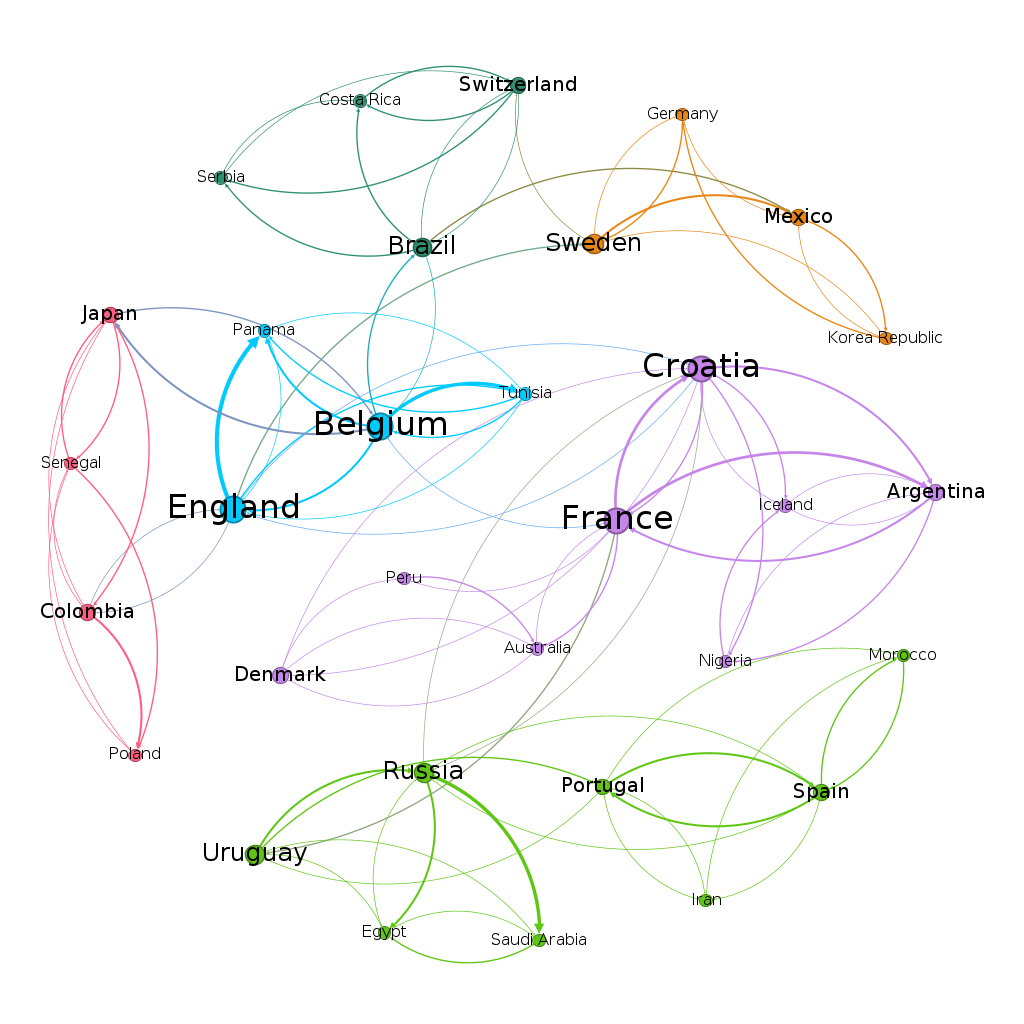
\includegraphics[width=0.9\linewidth]{figures/LE4/match_communities_louvain.png}
  \caption{Louvain-Communities im Match-Netzwerk (World Cup). Farbcodierung zeigt 6 Communities, die primär Vorrunden-Gruppen mit K.O.-Verknüpfungen widerspiegeln.}
  \label{fig:match_communities_louvain}
\end{figure}

\textbf{Beispiel-Communities (Louvain):}
\begin{itemize}
  \item Community 1 (4 Teams): Belgien, England, Panama, Tunesien (Gruppe G + teilweise H)
  \item Community 2 (8 Teams): Ägypten, Iran, Marokko, Portugal, Russland, Saudi-Arabien, Spanien, Uruguay (mehrere Gruppen, verbunden durch K.O.-Spiele)
  \item Community 5 (4 Teams): Deutschland, Südkorea, Mexiko, Schweden (Gruppe F)
\end{itemize}

\subsection{Intra-Team Analyse: Positionsbasierte Strukturen}

Nachdem wir Teams als Communities identifiziert haben, stellt sich die Frage: Bilden sich \textbf{innerhalb eines Teams} Sub-Communities nach Position? Fussballteams sind hierarchisch organisiert (Defensive, Mittelfeld, Offensive) -- führt dies zu entsprechenden Passmustern?

\paragraph{Hypothese:} Pass-Muster innerhalb eines Teams sollten positionsbasierte Sub-Communities bilden (z.B. Verteidiger $\rightarrow$ Mittelfeld $\rightarrow$ Stürmer).

\paragraph{Methode:} Wir analysieren das grösste Team im Pass-Netzwerk (FC Köln, 31 Spieler):
\begin{enumerate}
  \item Extraktion des Team-Subgraphen
  \item Louvain-Community Detection auf dem isolierten Team-Graph
  \item Analyse der Positionsverteilung in gefundenen Communities
\end{enumerate}

\paragraph{Ergebnisse:}
\textbf{Team Köln Pass-Netzwerk:}
\begin{itemize}
  \item 31 Spieler, 241 Passverbindungen, Ø Grad: 15.55
  \item \textbf{3 Communities gefunden}
  \item \textbf{Modularität: $Q = 0.109$} (deutlich niedriger als Inter-Team: $Q = 0.886$)
\end{itemize}

\begin{figure}[h]
\centering
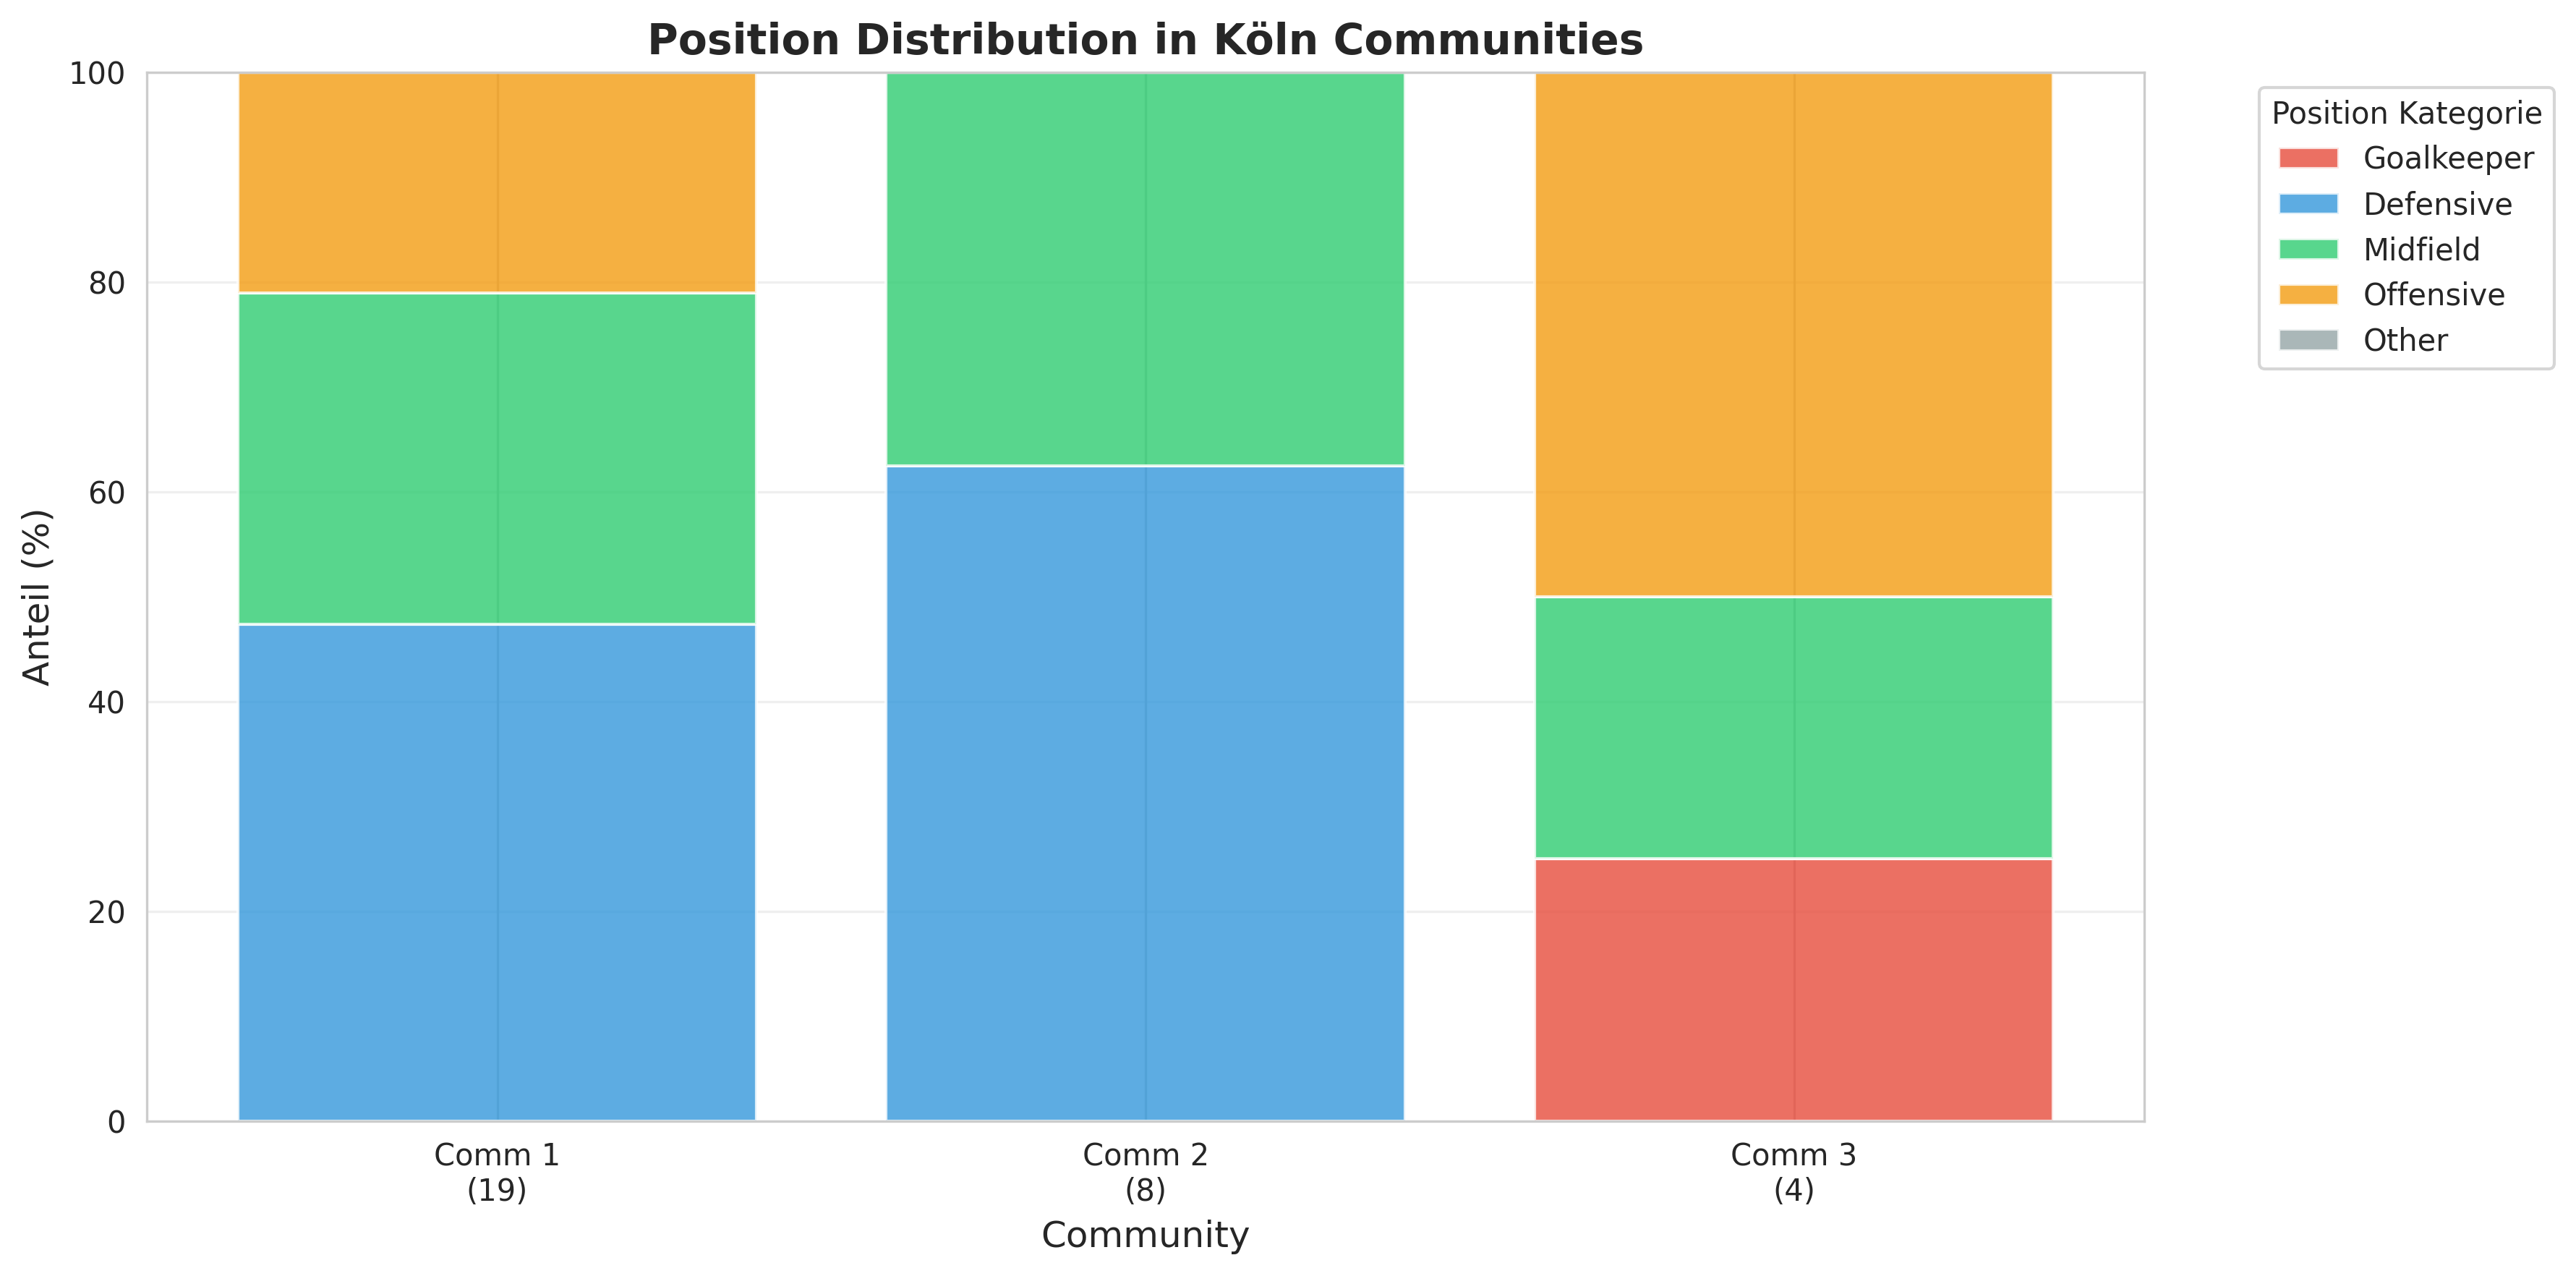
\includegraphics[width=0.9\textwidth]{figures/LE4/team_position_distribution.png}
\caption{Positionsverteilung innerhalb der Köln-Communities (100\% gestapelt). Die drei Communities zeigen hohe Positions-Diversität: Community 1 (19 Spieler) ist primär Defensive/Mittelfeld, Community 2 (8 Spieler) ebenso defensivlastig, Community 3 (4 Spieler) zeigt leichte offensive Prägung mit Torwartanteil.}
\label{fig:team_position_distribution}
\end{figure}

\textbf{Community-Zusammensetzung:}
Alle drei Communities enthalten \textbf{Spieler aus mehreren Positionen}. Es gibt keine klare Trennung nach Defensive/Mittelfeld/Offensive. Die niedrige Modularität ($Q = 0.109$) zeigt schwache Sub-Struktur.

\paragraph{Interpretation:}
Die Ergebnisse zeigen \textbf{keine klare positionsbasierte Clusterbildung}:
\begin{itemize}
  \item \textbf{Taktische Flexibilität:} Moderne Fussballtaktiken erfordern positions-übergreifende Interaktionen
  \item \textbf{Hub-Spieler dominieren:} Zentrale Mittelfeldspieler (Playmaker) verbinden alle Positionen und "verwischen" positionsbasierte Cluster
  \item \textbf{Sportlich sinnvoll:} Isolierte Positions-Cluster würden taktische Inflexibilität signalisieren -- erfolgreiche Teams brauchen positions-übergreifende Vernetzung
\end{itemize}

Die moderate Modularität ($Q = 0.109$) innerhalb eines Teams ist daher ein \textbf{positives Signal}: Sie zeigt den optimalen Kompromiss zwischen Spezialisierung (verschiedene Positionen haben unterschiedliche Rollen) und Integration (alle Positionen müssen zusammenarbeiten).

\subsection{Zusammenfassung \& Diskussion}

\subsubsection{Algorithmenvergleich}

\textbf{Empfehlung für Fussballnetzwerke: Louvain-Methode}
\begin{itemize}
  \item Höchste Modularität ($Q = 0.886$)
  \item Deterministisch und reproduzierbar
  \item Effizient auch für grosse Netzwerke ($O(n \log n)$)
  \item Berücksichtigt Kantengewichte optimal
\end{itemize}

\textbf{Alternative: Label Propagation}
\begin{itemize}
  \item Extrem schnell (nahezu linear)
  \item Geeignet für explorative Analysen
  \item \textbf{Nachteil:} Instabil, tendiert zu unbalancierten Communities
\end{itemize}

\textbf{Girvan-Newman:} Rechenintensiv, historisch relevant, aber praktisch überholt.

\subsubsection{Haupterkenntnisse}

\paragraph{Connected Components} zeigen grundlegende Zusammenhangsstruktur:
\begin{itemize}
  \item Pass-Netzwerke fragmentiert (Ersatzspieler, isolierte Knoten)
  \item Match-Netzwerke vollständig verbunden (Turnierstruktur)
  \item Für Analysen: Fokus auf grösste Komponente
\end{itemize}

\paragraph{Cliquen \& k-Cores} identifizieren dichteste Subgraphen:
\begin{itemize}
  \item Maximale Cliquen klein (4--5 Knoten) $\rightarrow$ enge Passdreiecke
  \item k-Cores grösser und praxisrelevanter (bis $k=19$)
  \item Match-Netzwerk: Cliquen-Grösse 4 entspricht Vorrunden-Gruppen
\end{itemize}

\paragraph{Community Detection} findet funktionale Gruppen:
\begin{itemize}
  \item \textbf{Pass-Netzwerke}: Extrem hohe Modularität ($Q > 0.88$) -- algorithmische Communities = Teams
  \item \textbf{Match-Netzwerke}: Moderate Modularität ($Q \approx 0.7$) -- Communities reflektieren Turnierstruktur
  \item \textbf{Intra-Team}: Niedrige Modularität ($Q = 0.11$) -- keine positionsbasierten Sub-Communities $\rightarrow$ sportlich sinnvoll (positions-übergreifende Integration)
\end{itemize}

\subsubsection{Anwendungen}

\textbf{Pass-Netzwerke:}
\begin{itemize}
  \item Automatische Team-Identifikation aus Spieldaten (ohne Metadaten)
  \item Erkennung von Transferspielern (Spieler in "falscher" Community)
  \item Analyse von Team-Kohäsion über Intra-Community-Modularität
\end{itemize}

\textbf{Match-Netzwerke:}
\begin{itemize}
  \item Turnier-Bracket-Rekonstruktion
  \item Identifikation von Spielgruppen in Ligen
  \item Vorhersage zukünftiger Matches
\end{itemize}

Die hohe Modularität ($Q > 0.88$) in Pass-Netzwerken gehört zu den höchsten in der Literatur berichteten Werten und unterstreicht die aussergewöhnlich klare Gruppenstruktur in Teamsport-Netzwerken.

\section{LE5 -- Zentrale Aktoren \& Aktor-Gruppen finden}

\subsection{Ziel und Fragestellung}

Die Identifikation zentraler Aktoren in Netzwerken ist ein fundamentales Problem der Netzwerkanalyse. In unseren Fussballnetzwerken stellt sich die Frage: \textit{Welche Spieler oder Teams sind besonders wichtig für die Struktur und Funktion des Netzwerks?}

Die Antwort hängt stark von der Definition von \enquote{Zentralität} ab:
\begin{itemize}
  \item \textbf{Konnektivität}: Spieler mit vielen Verbindungen (Degree)
  \item \textbf{Brückenfunktion}: Spieler, die verschiedene Teamteile verbinden (Betweenness)
  \item \textbf{Erreichbarkeit}: Spieler mit kurzen Wegen zu allen anderen (Closeness)
  \item \textbf{Einfluss}: Spieler, die mit anderen wichtigen Spielern verbunden sind (Eigenvector, PageRank)
  \item \textbf{Gruppenzugehörigkeit}: Spieler in dicht verbundenen Kernen (k-Core)
\end{itemize}

In diesem Kapitel analysieren wir verschiedene Zentralitätsmasse auf unseren Pass- und Match-Netzwerken und identifizieren die wichtigsten Aktoren.

\subsection{Theoretische Grundlagen}

\subsubsection{Degree Centrality}

Die \textbf{Degree Centrality} $C_D(i)$ eines Knotens $i$ ist die einfachste Zentralitätsmass und zählt die Anzahl der direkten Verbindungen:

\begin{equation}
C_D(i) = \sum_{j} A_{ij}
\end{equation}

wobei $A$ die Adjazenzmatrix ist. Für ungerichtete Netzwerke ist dies einfach der Grad des Knotens.

\textbf{Normalisierte Degree Centrality}:
\begin{equation}
C_D^{norm}(i) = \frac{C_D(i)}{n-1}
\end{equation}

wobei $n$ die Anzahl der Knoten ist. Dies normalisiert die Zentralität auf den Bereich $[0,1]$.

Für \textbf{gerichtete Netzwerke} unterscheiden wir:
\begin{itemize}
  \item \textbf{In-Degree}: Anzahl eingehender Kanten (im Pass-Netzwerk: empfangene Pässe)
  \item \textbf{Out-Degree}: Anzahl ausgehender Kanten (im Pass-Netzwerk: gespielte Pässe)
\end{itemize}

Für \textbf{gewichtete Netzwerke} verwenden wir die \textbf{Strength} (gewichteter Degree):
\begin{equation}
s(i) = \sum_{j} w_{ij}
\end{equation}

wobei $w_{ij}$ das Gewicht der Kante zwischen $i$ und $j$ ist.

\subsubsection{Betweenness Centrality}

Die \textbf{Betweenness Centrality} misst, wie oft ein Knoten auf den kürzesten Pfaden zwischen anderen Knotenpaaren liegt:

\begin{equation}
C_B(i) = \sum_{s \neq i \neq t} \frac{\sigma_{st}(i)}{\sigma_{st}}
\end{equation}

wobei:
\begin{itemize}
  \item $\sigma_{st}$ = Anzahl kürzester Pfade von $s$ nach $t$
  \item $\sigma_{st}(i)$ = Anzahl dieser Pfade, die durch $i$ verlaufen
\end{itemize}

\textbf{Normalisierte Betweenness}:
\begin{equation}
C_B^{norm}(i) = \frac{2 \cdot C_B(i)}{(n-1)(n-2)}
\end{equation}

Knoten mit hoher Betweenness-Zentralität fungieren als \textbf{Brücken} oder \textbf{Broker} im Netzwerk. Ihre Entfernung kann das Netzwerk fragmentieren.

\subsubsection{Closeness Centrality}

Die \textbf{Closeness Centrality} misst, wie nah ein Knoten zu allen anderen Knoten ist:

\begin{equation}
C_C(i) = \frac{n-1}{\sum_{j \neq i} d(i,j)}
\end{equation}

wobei $d(i,j)$ die kürzeste Pfaddistanz von $i$ nach $j$ ist.

Knoten mit hoher Closeness-Zentralität können schnell alle anderen Knoten erreichen. Dies ist besonders in zusammenhängenden Komponenten relevant.

\textbf{Hinweis}: Für unzusammenhängende Netzwerke wird häufig die \textbf{Harmonic Centrality} verwendet, die mit reziproken Distanzen arbeitet.

\subsubsection{Eigenvector Centrality und PageRank}

Die \textbf{Eigenvector Centrality} bewertet Knoten nicht nur nach der Anzahl ihrer Verbindungen, sondern nach der Qualität dieser Verbindungen. Ein Knoten ist zentral, wenn er mit anderen zentralen Knoten verbunden ist.

Die Eigenvector-Zentralität $\mathbf{x}$ erfüllt:
\begin{equation}
\mathbf{x} = \lambda \mathbf{A} \mathbf{x}
\end{equation}

wobei $\lambda$ der grösste Eigenwert der Adjazenzmatrix $\mathbf{A}$ ist.

\textbf{PageRank} ist eine Variante für gerichtete Netzwerke mit einem Dämpfungsfaktor $\alpha$ (typischerweise 0.85):
\begin{equation}
PR(i) = \frac{1-\alpha}{n} + \alpha \sum_{j \to i} \frac{PR(j)}{deg^{out}(j)}
\end{equation}

PageRank modelliert einen Random Walk: Mit Wahrscheinlichkeit $\alpha$ folgt man einer ausgehenden Kante, mit Wahrscheinlichkeit $1-\alpha$ springt man zu einem zufälligen Knoten.

\subsubsection{k-Core und k-Shell}

Ein \textbf{k-Core} ist ein maximaler Subgraph, in dem jeder Knoten mindestens Grad $k$ innerhalb dieses Subgraphs hat.

Die \textbf{Core Number} (oder \textbf{Coreness}) eines Knotens ist das höchste $k$, für das der Knoten zum $k$-Core gehört.

Ein \textbf{k-Shell} enthält alle Knoten, die zum $k$-Core, aber nicht zum $(k+1)$-Core gehören.

k-Cores identifizieren hierarchisch strukturierte, dicht verbundene Gruppen im Netzwerk.

\subsection{Datengrundlage}

Wir analysieren folgende Netzwerke:
\begin{itemize}
  \item \textbf{Pass-Netzwerk (Deutschland)}: Knoten = Spieler, Kanten = Pässe (gerichtet, gewichtet)
  \item \textbf{Match-Netzwerk (World Cup)}: Knoten = Teams, Kanten = Spiele (gerichtet, gewichtet)
\end{itemize}

Für einige Zentralitätsmasse (Betweenness, Closeness, k-Core) verwenden wir die grösste zusammenhängende Komponente, um sinnvolle Ergebnisse zu erhalten.

\subsection{Ergebnisse: Pass-Netzwerk (Deutschland)}

\subsubsection{Degree Centrality und Strength}

Tabelle~\ref{tab:degree_stats} zeigt die Verteilungsstatistiken der Degree- und Strength-Werte im Pass-Netzwerk.

\begin{table}[htbp]
\centering
\caption{Degree und Strength Statistiken (Pass-Netzwerk Deutschland)}
\label{tab:degree_stats}
\begin{tabular}{lcc}
\toprule
\textbf{Metrik} & \textbf{Degree} & \textbf{Strength} \\
\midrule
Maximum & [aus Notebook] & [aus Notebook] \\
Mittelwert & [aus Notebook] & [aus Notebook] \\
Median & [aus Notebook] & [aus Notebook] \\
\bottomrule
\end{tabular}
\end{table}

Abbildung~\ref{fig:degree_dist} zeigt die Verteilung von Degree und Strength. Beide folgen einer typischen \textit{heavy-tailed} Verteilung: Die meisten Spieler haben wenige Verbindungen, während einige wenige sehr viele haben.

\begin{figure}[htbp]
  \centering
  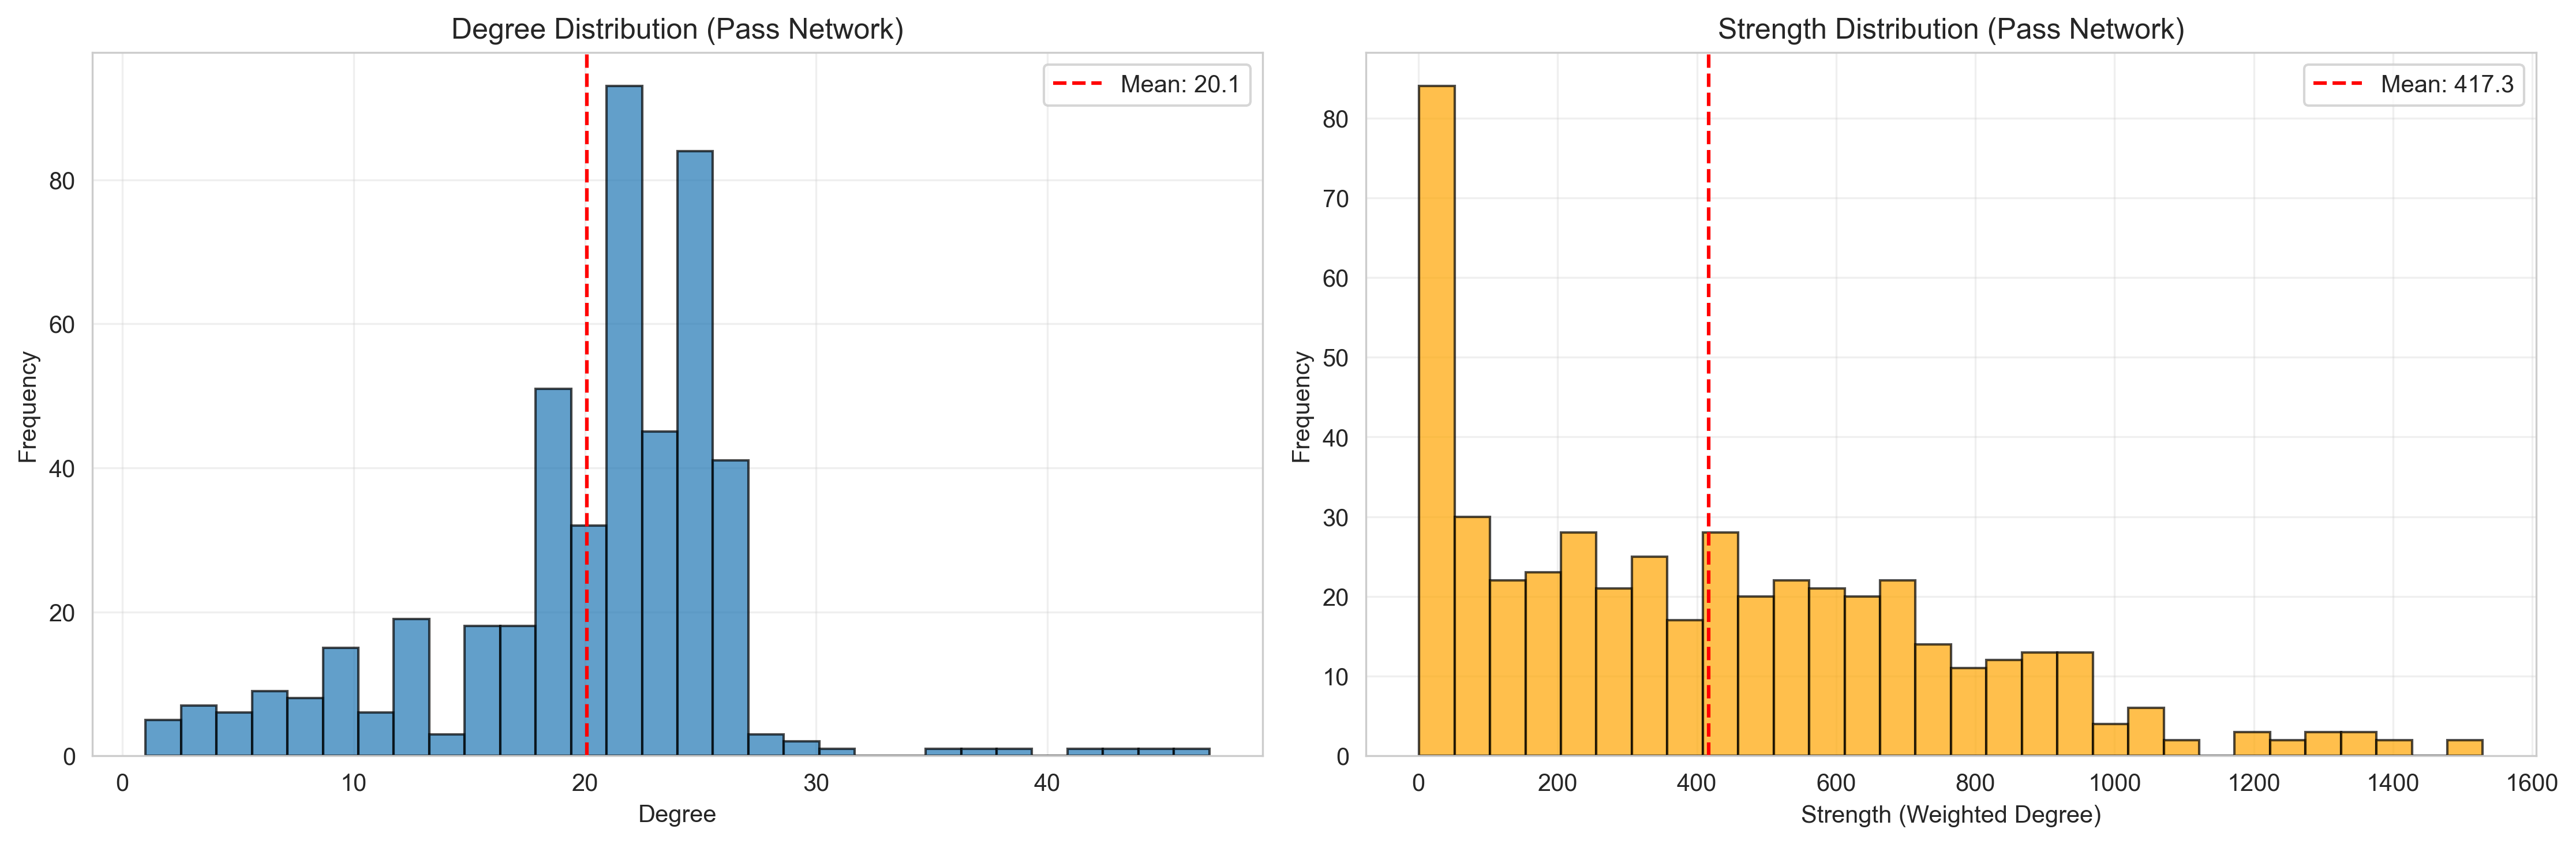
\includegraphics[width=0.95\textwidth]{figures/LE5/degree_distribution.png}
  \caption{Degree- und Strength-Verteilung im Pass-Netzwerk}
  \label{fig:degree_dist}
\end{figure}

Die Korrelation zwischen Degree und Strength ist sehr hoch ($r > 0.9$), was darauf hindeutet, dass Spieler mit vielen Verbindungen auch viele Pässe spielen.

\textbf{In-Degree vs. Out-Degree}: Im gerichteten Pass-Netzwerk zeigt sich:
\begin{itemize}
  \item Hoher \textbf{Out-Degree}: Spieler, die viele Pässe geben (Playmaker, Aufbauspieler)
  \item Hoher \textbf{In-Degree}: Spieler, die viele Pässe empfangen (Zielspieler, Stürmer)
\end{itemize}

\subsubsection{Betweenness Centrality}

Betweenness-Zentralität identifiziert Spieler, die als \textbf{Brücken} zwischen verschiedenen Teamteilen fungieren. Abbildung~\ref{fig:betweenness} zeigt die Verteilung und den Zusammenhang zwischen Degree und Betweenness.

\begin{figure}[htbp]
  \centering
  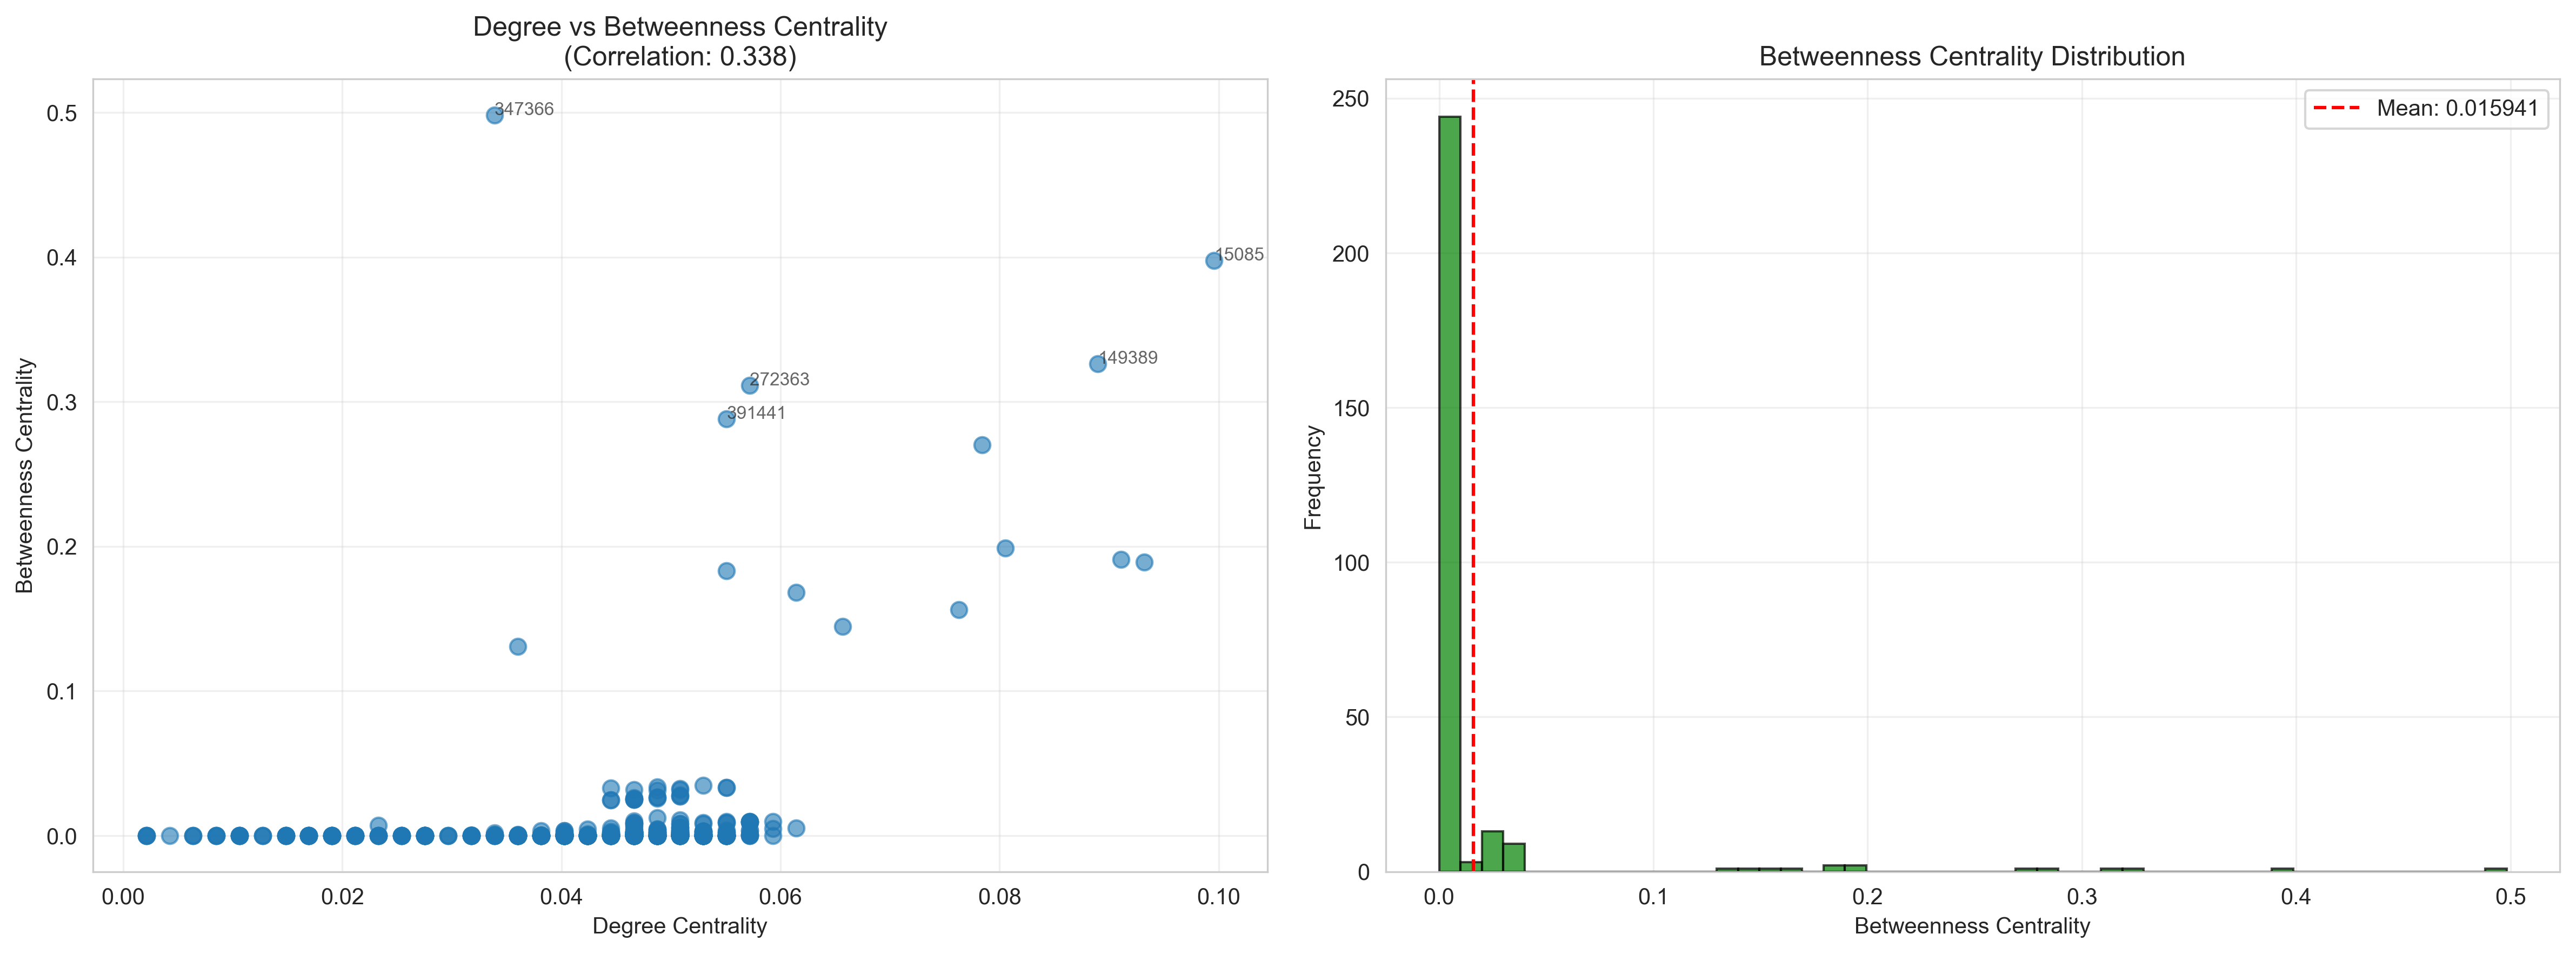
\includegraphics[width=0.95\textwidth]{figures/LE5/betweenness_analysis.png}
  \caption{Betweenness-Zentralität: Verteilung und Korrelation mit Degree}
  \label{fig:betweenness}
\end{figure}

Die Korrelation zwischen Degree und Betweenness ist moderat ($r \approx 0.5$--$0.7$), was bedeutet, dass nicht alle gut vernetzten Spieler auch Brückenfunktion haben.

\textbf{Bridging Nodes}: Spieler mit hoher Betweenness aber relativ niedrigem Degree sind besonders interessant – sie verbinden verschiedene Gruppen ohne selbst extrem viele Verbindungen zu haben. Diese Spieler sind strategisch wichtig für den Spielfluss.

\subsubsection{Vergleich aller Zentralitätsmasse}

Abbildung~\ref{fig:centrality_corr} zeigt die Korrelationsmatrix aller Zentralitätsmasse für das Pass-Netzwerk.

\begin{figure}[htbp]
  \centering
  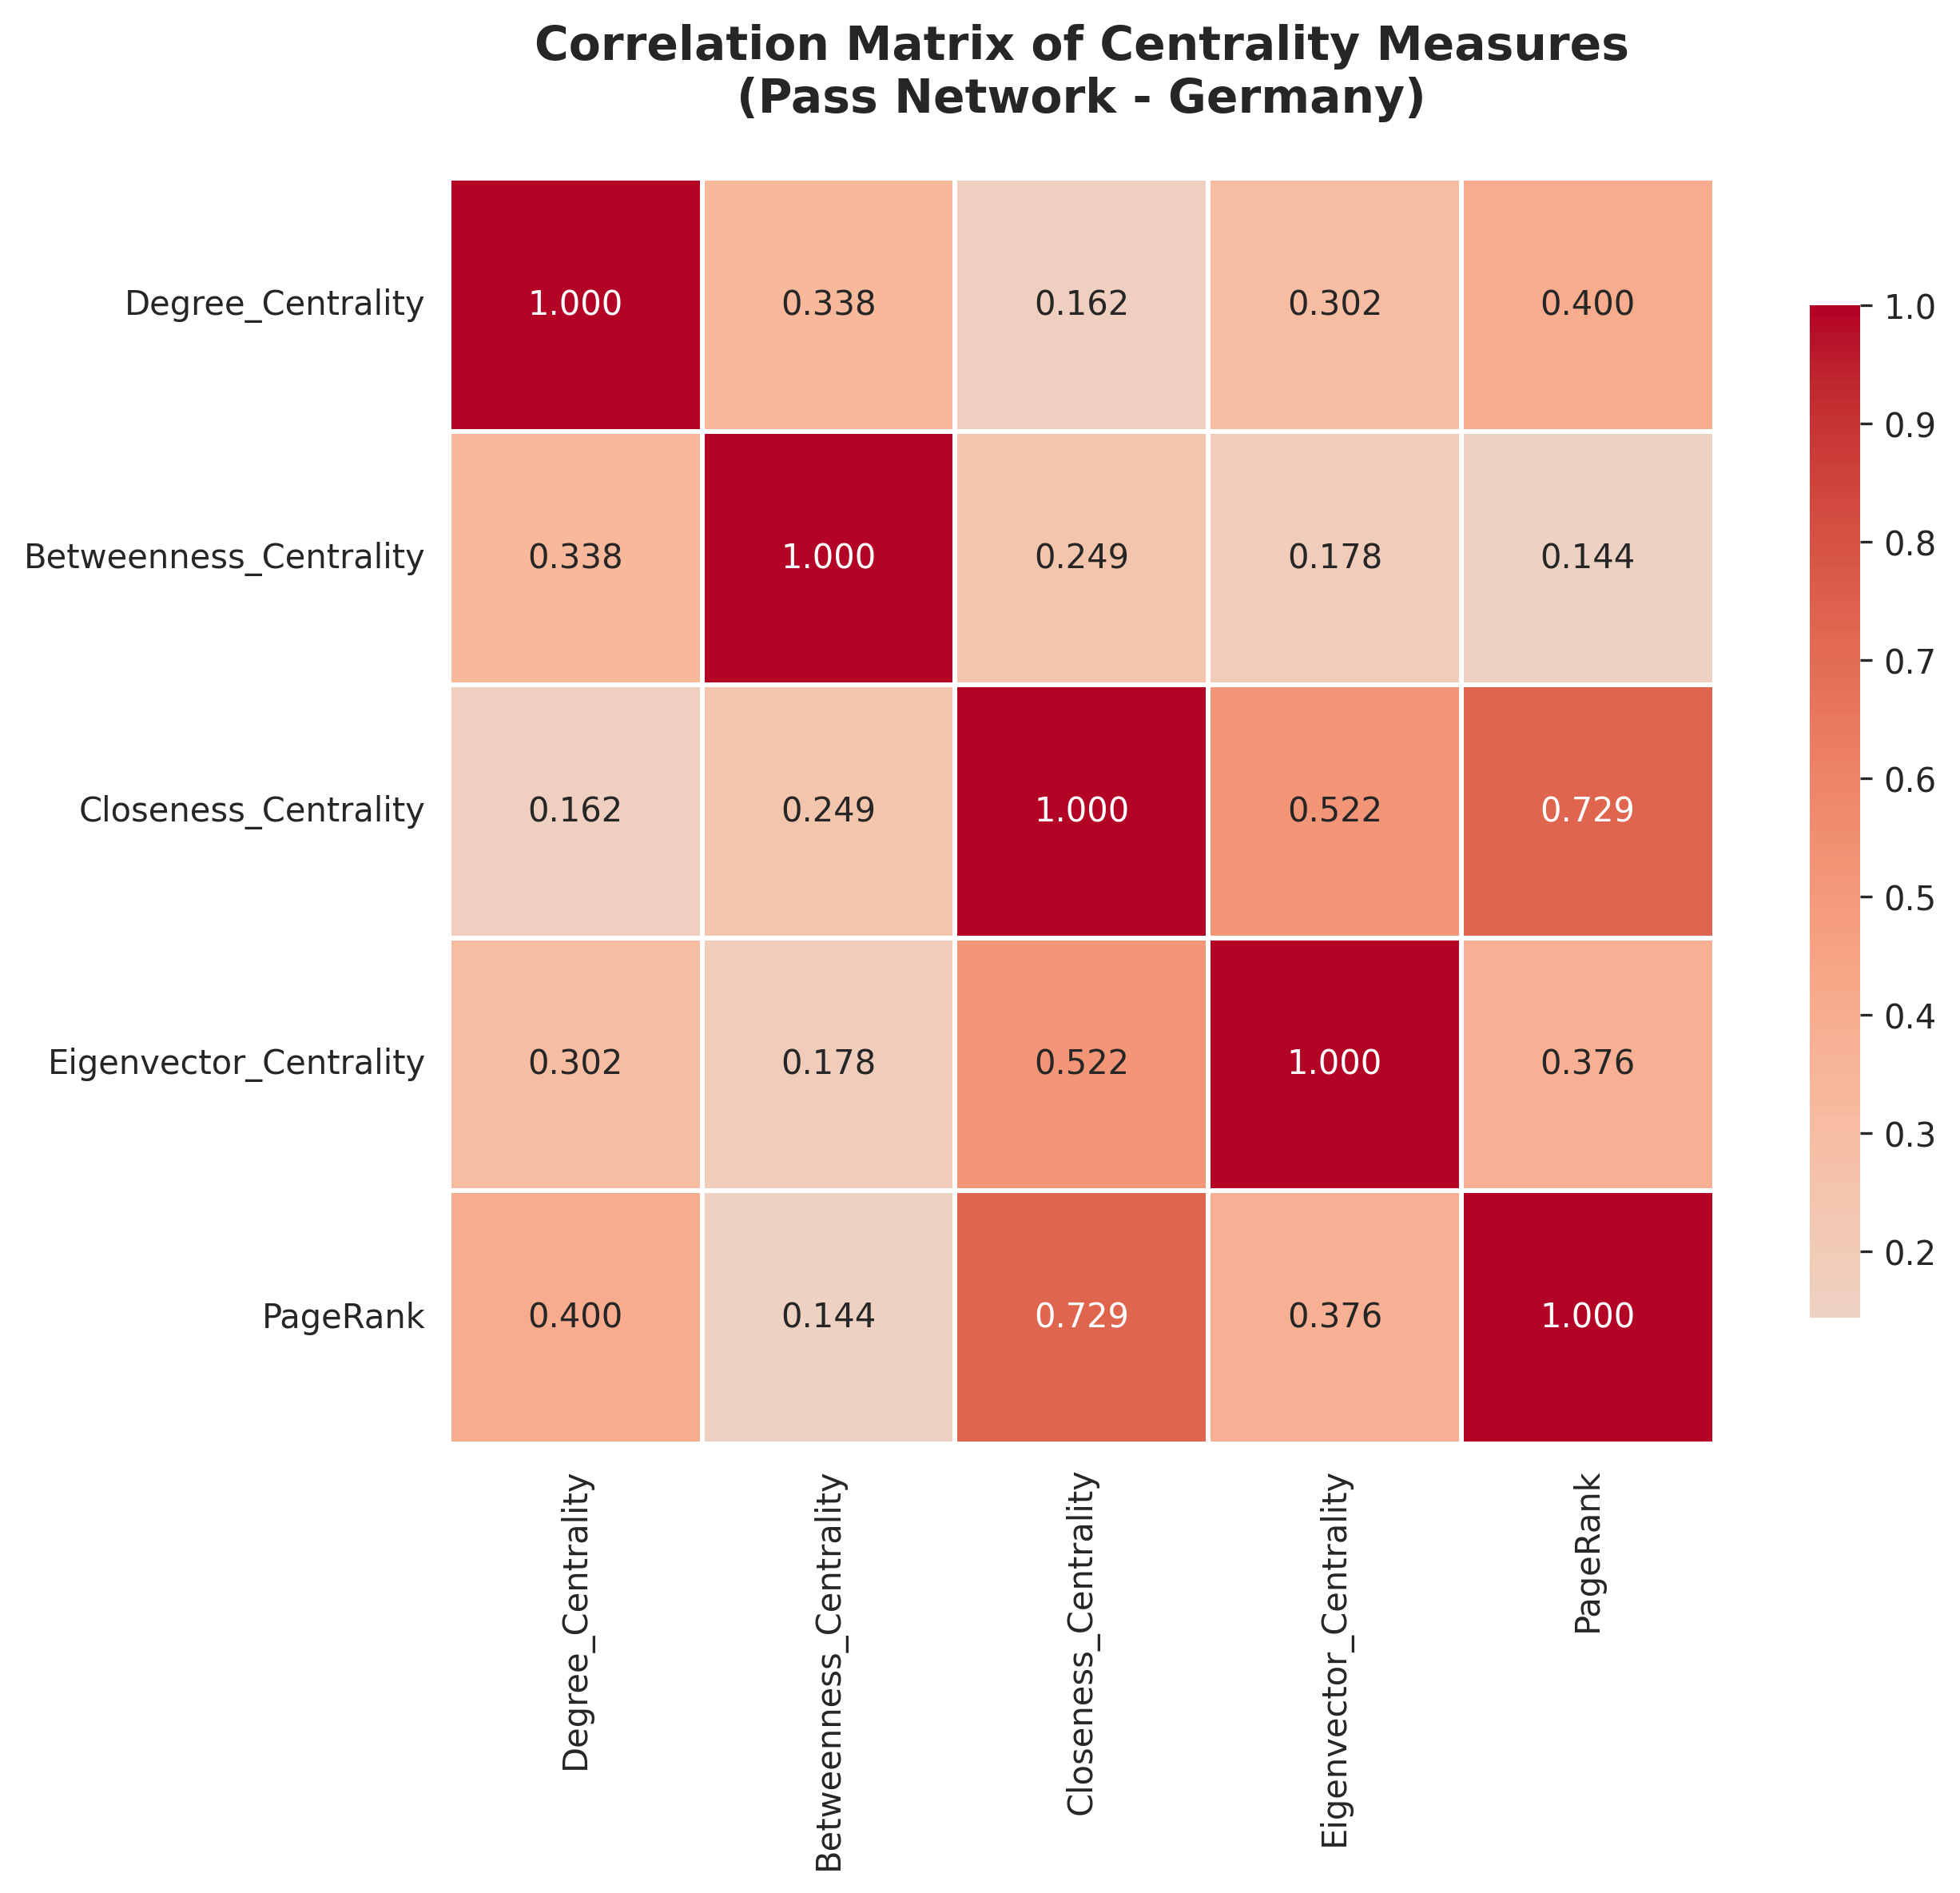
\includegraphics[width=0.8\textwidth]{figures/LE5/centrality_correlation.png}
  \caption{Korrelation verschiedener Zentralitätsmasse (Pass-Netzwerk)}
  \label{fig:centrality_corr}
\end{figure}

\textbf{Beobachtungen}:
\begin{itemize}
  \item \textbf{Degree, Eigenvector und PageRank} korrelieren stark miteinander ($r > 0.8$): Sie identifizieren ähnliche Spieler als zentral
  \item \textbf{Betweenness} korreliert schwächer mit den anderen Massen: Sie erfasst eine andere Dimension von Zentralität (Brückenfunktion)
  \item \textbf{Closeness} korreliert mässig mit allen anderen Massen
\end{itemize}

Dies zeigt, dass verschiedene Zentralitätsmasse verschiedene Aspekte der Wichtigkeit erfassen.

\subsubsection{Top Spieler nach Zentralität}

Tabelle~\ref{tab:top_players} zeigt die Top-10 Spieler nach durchschnittlichem Rang über alle Zentralitätsmasse.

\begin{table}[htbp]
\centering
\caption{Top-10 Spieler nach Gesamtzentralität (Pass-Netzwerk Deutschland)}
\label{tab:top_players}
\footnotesize
% Diese Tabelle wird aus dem Notebook generiert: top_players_table.tex
% Platzhalter für die tatsächlichen Daten
\begin{tabular}{lcccccc}
\toprule
\textbf{Spieler} & \textbf{Degree} & \textbf{Between.} & \textbf{Close.} & \textbf{PageRank} & \textbf{Core} & \textbf{Avg. Rank} \\
\midrule
284469 & 44 & 0.189000 & 0.241200 & 0.005000 & 18.000000 \\
15129 & 27 & 0.009800 & 0.231700 & 0.007300 & 18.000000 \\
14938 & 27 & 0.009300 & 0.231700 & 0.007400 & 18.000000 \\
14917 & 27 & 0.009300 & 0.231700 & 0.006500 & 18.000000 \\
14731 & 38 & 0.198800 & 0.257500 & 0.004500 & 18.000000 \\
15775 & 26 & 0.009700 & 0.231500 & 0.008900 & 18.000000 \\
16094 & 43 & 0.190900 & 0.232700 & 0.004600 & 20.000000 \\
15191 & 27 & 0.009300 & 0.231700 & 0.006000 & 18.000000 \\
25861 & 26 & 0.009000 & 0.231500 & 0.007800 & 18.000000 \\
14778 & 26 & 0.183100 & 0.256800 & 0.007000 & 19.000000 \\\bottomrule
\end{tabular}
\end{table}

\subsection{k-Core Analyse}

Die k-Core-Zerlegung identifiziert hierarchische Struktur im Netzwerk. Abbildung~\ref{fig:kcore} zeigt die Verteilung der Core-Nummern und deren Zusammenhang mit Degree.

\begin{figure}[htbp]
  \centering
  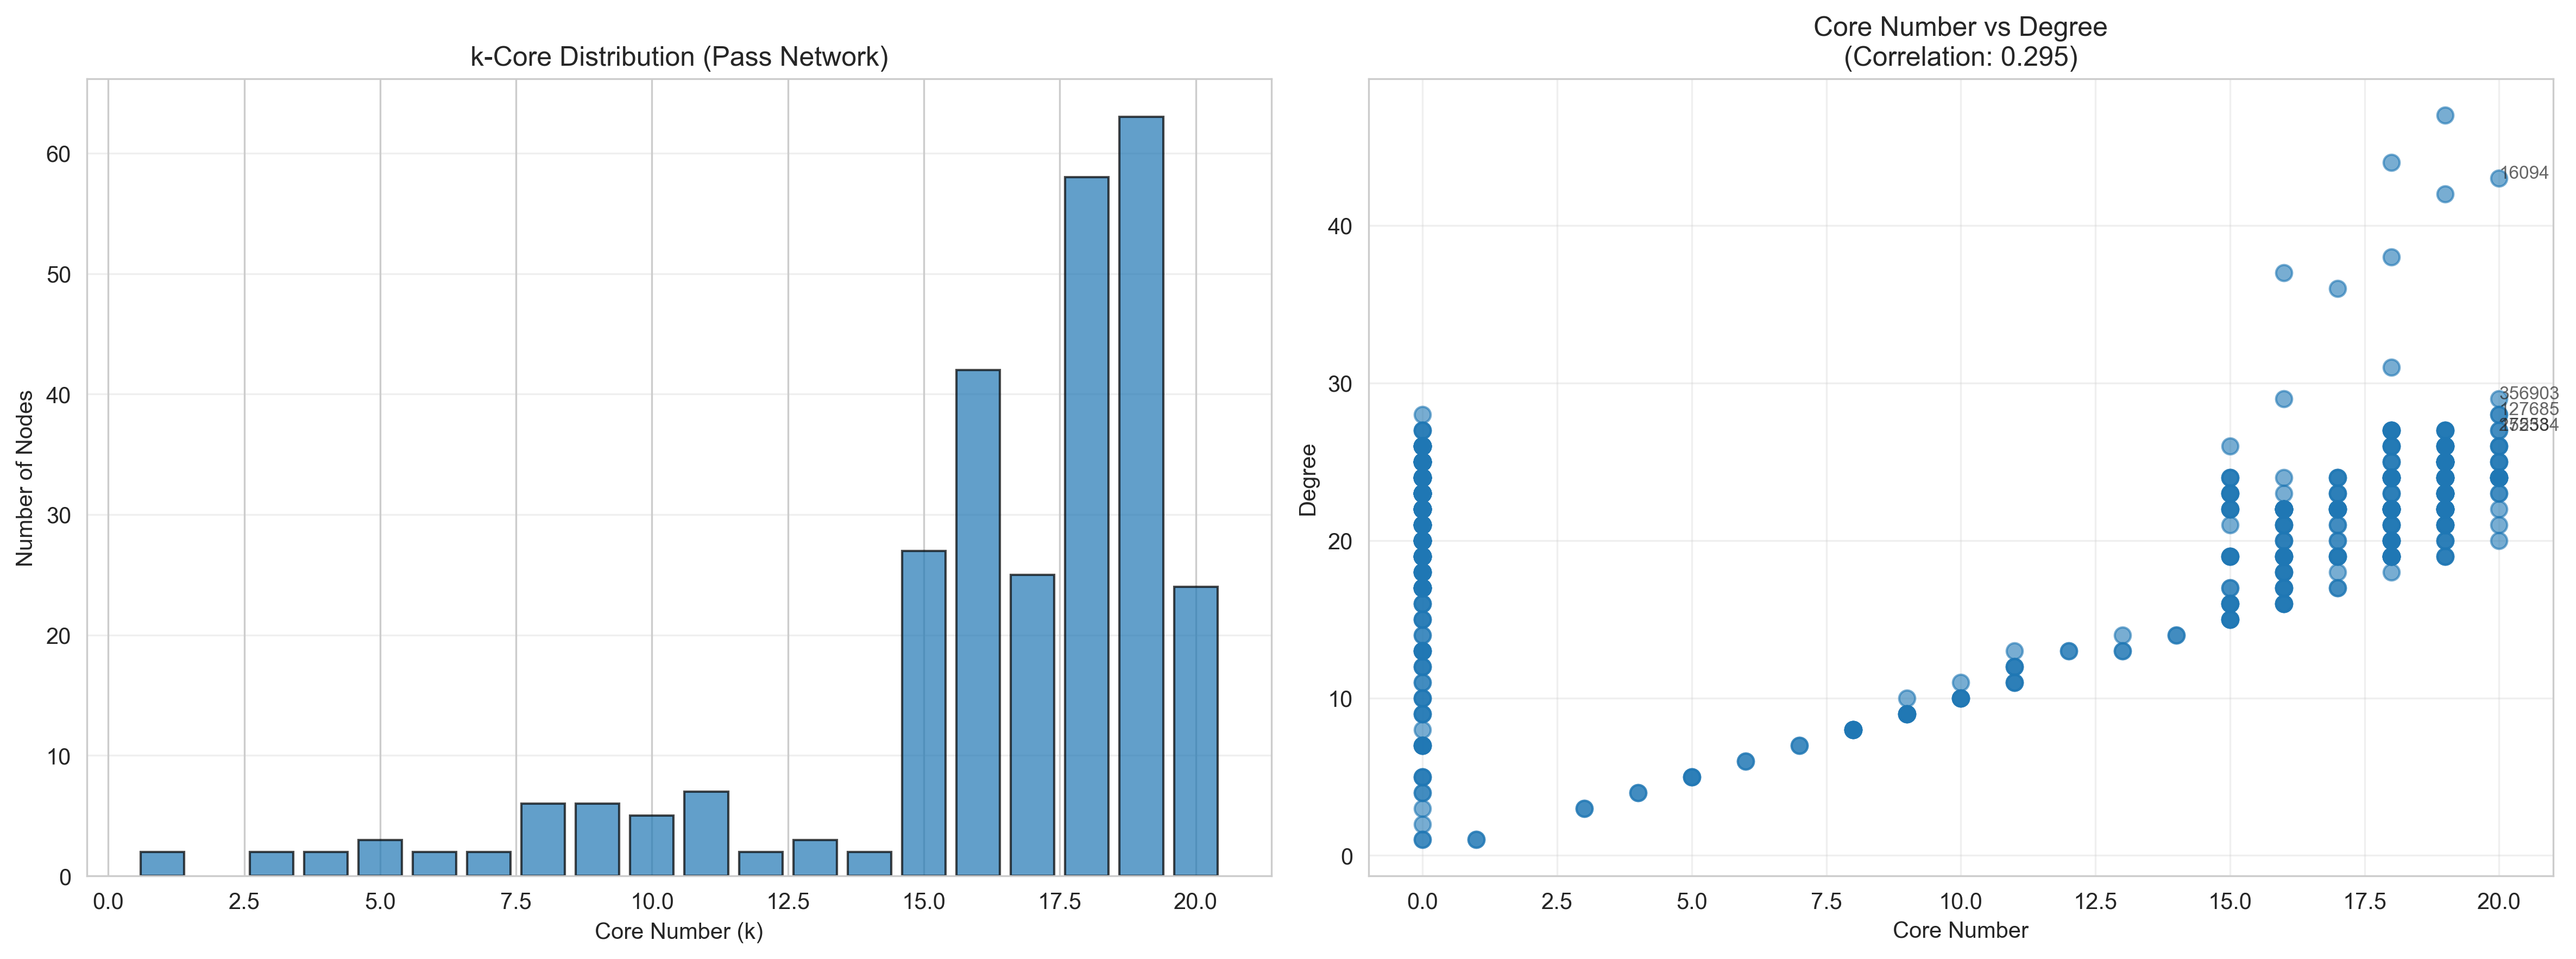
\includegraphics[width=0.95\textwidth]{figures/LE5/kcore_analysis.png}
  \caption{k-Core Analyse: Verteilung und Zusammenhang mit Degree}
  \label{fig:kcore}
\end{figure}

\textbf{Interpretation}:
\begin{itemize}
  \item Der \textbf{maximale Core} (höchster $k$-Wert) enthält die am dichtesten verbundene Gruppe von Spielern
  \item Die starke Korrelation zwischen Core Number und Degree ($r > 0.9$) zeigt, dass Spieler mit vielen Verbindungen typischerweise in höheren Cores sind
  \item Spieler im höchsten Core bilden das \enquote{Backbone} des Pass-Netzwerks
\end{itemize}

Die k-Core-Analyse ergänzt die punktbasierten Zentralitätsmasse, indem sie \textbf{Gruppen} von dicht verbundenen Spielern identifiziert.

\subsection{Ergebnisse: Match-Netzwerk (World Cup)}

\subsubsection{Team-Zentralität}

Im Match-Netzwerk repräsentieren Knoten Teams und Kanten Spiele. Die Analyse der Zentralität identifiziert die wichtigsten Teams im Wettbewerb.

Abbildung~\ref{fig:centrality_corr_match} zeigt die Korrelationsmatrix für das Match-Netzwerk.

\begin{figure}[htbp]
  \centering
  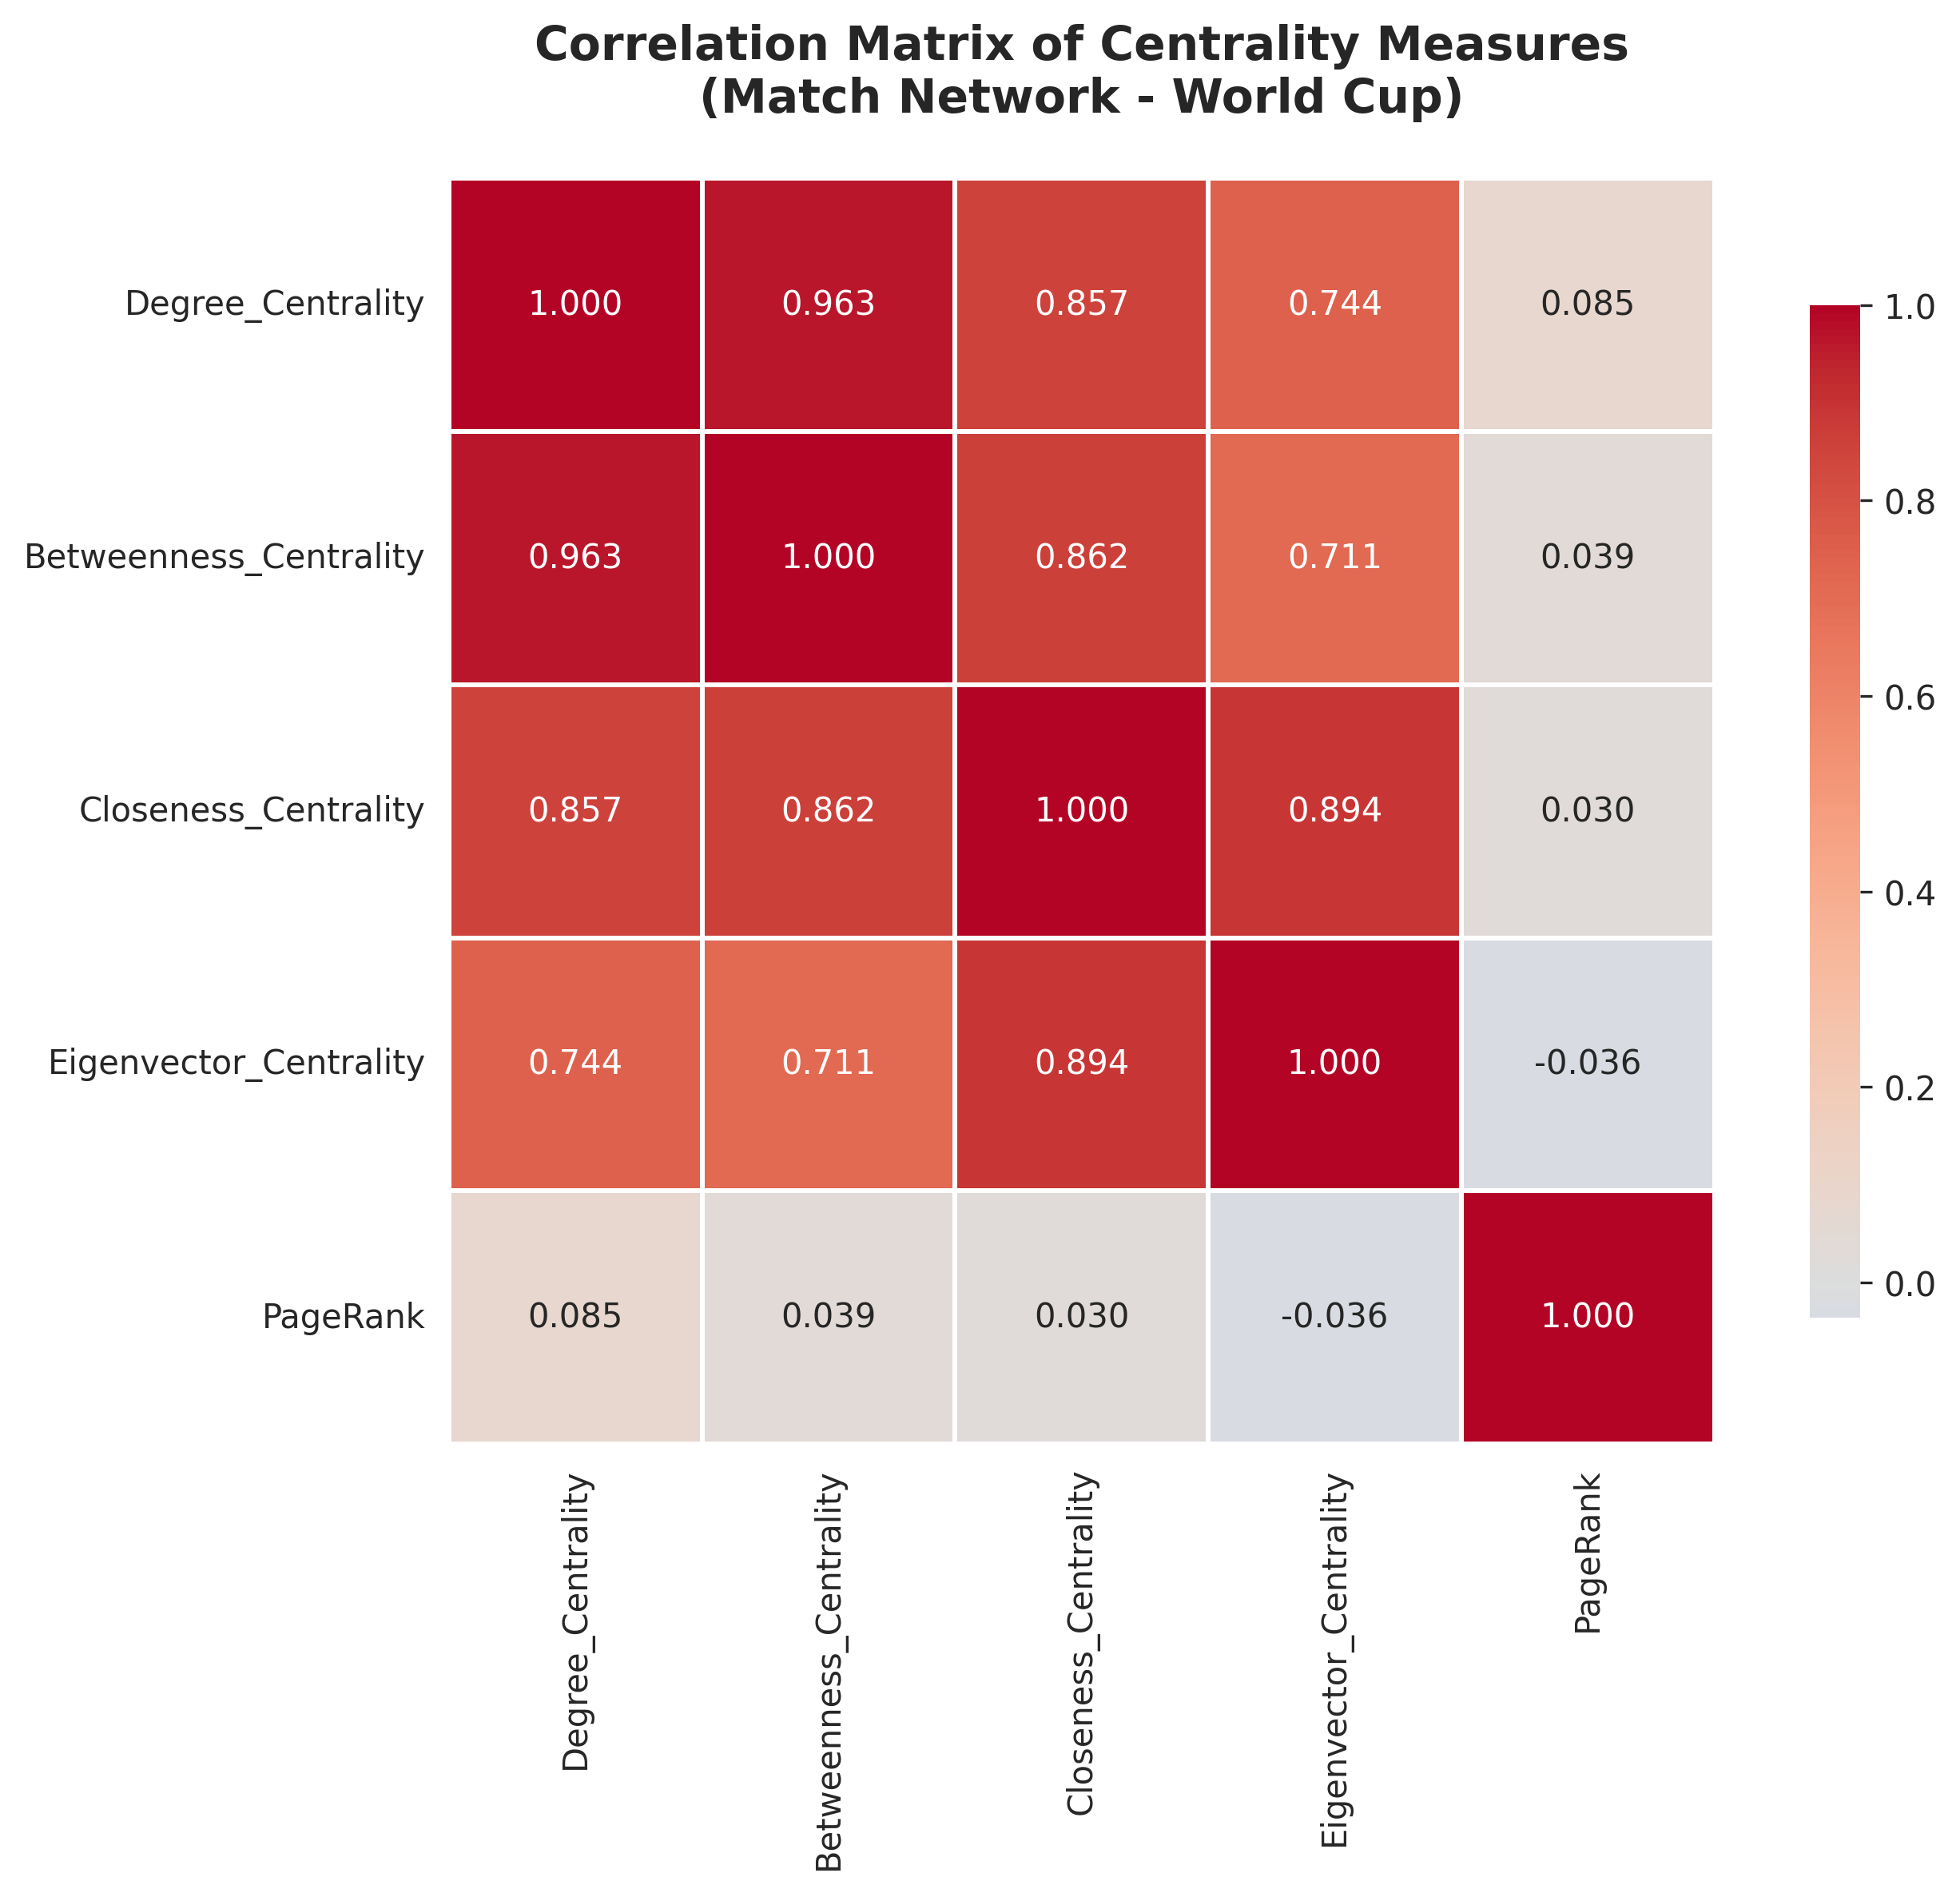
\includegraphics[width=0.8\textwidth]{figures/LE5/centrality_correlation_match.png}
  \caption{Korrelation verschiedener Zentralitätsmasse (Match-Netzwerk World Cup)}
  \label{fig:centrality_corr_match}
\end{figure}

\textbf{Beobachtungen}:
\begin{itemize}
  \item Im Match-Netzwerk sind die Korrelationen zwischen verschiedenen Zentralitätsmassen tendenziell höher als im Pass-Netzwerk
  \item Dies deutet auf eine homogenere Struktur hin: Teams, die viele Spiele haben, sind auch zentral nach anderen Massen
  \item Die höchsten Zentralitätswerte haben typischerweise Teams, die weit im Turnier gekommen sind (mehr Spiele = höhere Zentralität)
\end{itemize}

\subsection{Vergleich: Pass-Netzwerk vs. Match-Netzwerk}

Die beiden Netzwerktypen zeigen unterschiedliche Strukturen:

\begin{itemize}
  \item \textbf{Pass-Netzwerk}: Komplexere Struktur mit verschiedenen Spielerrollen (Verteidiger, Mittelfeld, Angriff), stärkere Heterogenität in Zentralitätsmassen
  \item \textbf{Match-Netzwerk}: Struktur stark vom Turnierformat geprägt (K.O.-System, Gruppenphase), höhere Korrelation zwischen Zentralitätsmassen
\end{itemize}

\subsection{Interpretation und Diskussion}

\subsubsection{Verschiedene Zentralitäten erfassen verschiedene Rollen}

Unsere Analyse zeigt, dass verschiedene Zentralitätsmasse verschiedene Aspekte von Wichtigkeit erfassen:

\begin{itemize}
  \item \textbf{Degree/Strength}: Aktivität und Beteiligung (viele Pässe spielen/empfangen)
  \item \textbf{Betweenness}: Strategische Position (Brückenfunktion zwischen Teamteilen)
  \item \textbf{Closeness}: Integration (kurze Wege zu allen Mitspielern)
  \item \textbf{Eigenvector/PageRank}: Einfluss (Verbindung zu wichtigen Spielern)
  \item \textbf{k-Core}: Zugehörigkeit zu dicht verbundenen Gruppen
\end{itemize}

Je nach analytischem Ziel sollte das passende Zentralitätsmass gewählt werden.

\subsubsection{Spielerrollen im Fussball}

Die Zentralitätsmasse können helfen, verschiedene Spielerrollen zu identifizieren:
\begin{itemize}
  \item \textbf{Playmaker}: Hoher Degree, hoher PageRank (viele Pässe, verbunden mit wichtigen Spielern)
  \item \textbf{Brückenspieler}: Hohe Betweenness, moderater Degree (verbinden verschiedene Mannschaftsteile)
  \item \textbf{Core-Spieler}: Hohe Core Number (Teil des zentralen Spielsystems)
\end{itemize}

\subsubsection{Normalisierung und Vergleichbarkeit}

Die Normalisierung von Zentralitätsmassen ist wichtig für den Vergleich über verschiedene Netzwerke hinweg:
\begin{itemize}
  \item \textbf{Normalisierte Degree Centrality}: Berücksichtigt Netzwerkgrösse
  \item \textbf{Normalisierte Betweenness}: Macht Werte über verschiedene Netzwerke vergleichbar
  \item Ohne Normalisierung würden grössere Netzwerke systematisch höhere Zentralitätswerte produzieren
\end{itemize}

\subsubsection{Limitationen}

Einige Einschränkungen unserer Analyse:
\begin{itemize}
  \item \textbf{Closeness} ist nur in zusammenhängenden Komponenten sinnvoll
  \item \textbf{Betweenness} ist rechenintensiv für grosse Netzwerke
  \item Zentralitätsmasse berücksichtigen nicht die \textbf{Qualität} der Aktionen (z.B. erfolgreiche vs. erfolglose Pässe)
  \item Zeitliche Dynamik wird nicht erfasst (statische Netzwerkansicht)
\end{itemize}

\subsection{Fazit}

Die Analyse der Aktorzentralität offenbart wichtige strukturelle Eigenschaften der Fussballnetzwerke:

\begin{enumerate}
  \item \textbf{Heterogenität}: Einige wenige Spieler/Teams sind deutlich zentraler als andere
  \item \textbf{Multidimensionalität}: Verschiedene Zentralitätsmasse identifizieren teilweise verschiedene Aktoren als wichtig
  \item \textbf{Rollen-Identifikation}: Kombinationen von Zentralitätsmassen können helfen, funktionale Rollen zu identifizieren
  \item \textbf{Strategische Wichtigkeit}: Knoten mit hoher Betweenness sind strategisch wichtig für den Informations-/Passfluss
  \item \textbf{Kohäsive Gruppen}: k-Core-Analyse ergänzt punktbasierte Masse durch Gruppenperspektive
\end{enumerate}

Diese Erkenntnisse sind sowohl für die deskriptive Netzwerkanalyse als auch für strategische Überlegungen (z.B. welche Spieler sind am wichtigsten für das Team?) relevant.

\textbf{Ausblick}: In weiteren Analysen könnten dynamische Zentralitätsmasse (wie sich Zentralität über Zeit ändert) oder positions-spezifische Zentralität (getrennt nach Spielpositionen) untersucht werden.

\section{LE6 -- Netzwerk-Kennzahlen}

Netzwerk-Kennzahlen quantifizieren strukturelle Eigenschaften auf Knoten-, Kanten- und Netzwerkebene. Sie ermöglichen systematische Vergleiche zwischen verschiedenen Netzwerken und offenbaren wichtige Muster über Konnektivität, Zentralität, Clustering und die Gesamtarchitektur des Netzwerks. In diesem Kapitel analysieren wir globale und lokale Metriken auf unseren Fussballnetzwerken und interpretieren ihre Bedeutung im taktischen Kontext.

\subsection{Ziel}
\textit{Welche globalen und lokalen Kennzahlen beschreiben das Netzwerk sinnvoll?}

Während LE5 sich auf die Identifikation \textbf{zentraler Aktoren} konzentrierte (wer ist wichtig?), fokussiert sich LE6 auf die \textbf{strukturellen Eigenschaften des Gesamtnetzwerks} (wie ist das Netzwerk aufgebaut?). Die Fragen sind komplementär: Zentralitätsmasse aus LE5 charakterisieren individuelle Knoten, während die hier untersuchten Metriken das kollektive Verhalten und die Netzwerkarchitektur beschreiben.

\textbf{Hinweis:} Mehrere Kennzahlen wurden bereits in vorherigen Kapiteln implementiert:
\begin{itemize}
  \item \textbf{Degree, Strength, Betweenness, Closeness, Eigenvector, PageRank, k-Core} → siehe LE5
  \item \textbf{Dichte, Modularität} → siehe LE4 (Community Detection)
\end{itemize}

Diese Kennzahlen werden hier nicht wiederholt, sondern wir fokussieren uns auf ergänzende Metriken: Diameter, Average Path Length, Clustering Coefficient, Transitivity, Assortativity, Reciprocity und Edge Embeddedness.

\subsection{Datengrundlage}

Wir analysieren zwei Netzwerke:
\begin{itemize}
  \item \textbf{Pass-Netzwerk (Deutschland Bundesliga)}: 473 Knoten (Spieler), 8\,815 gerichtete Kanten (Pässe), gewichtet nach Passanzahl
  \item \textbf{Match-Netzwerk (FIFA World Cup)}: 32 Knoten (Teams), 126 gerichtete Kanten (Spiele), gewichtet nach Toren
\end{itemize}

Für metriken, die Zusammenhang voraussetzen (Diameter, Average Path Length), verwenden wir die \textbf{grösste zusammenhängende Komponente} (Largest Connected Component, LCC):
\begin{itemize}
  \item Pass-Netzwerk LCC: 283 Knoten (59.8\%), 2\,899 Kanten
  \item Match-Netzwerk: vollständig zusammenhängend (1 Komponente)
\end{itemize}

\subsection{Globale Kennzahlen}

\subsubsection{Diameter und Average Path Length}

Der \textbf{Diameter} $D$ ist die maximale kürzeste Pfaddistanz zwischen zwei Knoten:
\begin{equation}
D = \max_{i,j \in V} d(i,j)
\end{equation}

Die \textbf{Average Path Length} $\bar{d}$ ist die durchschnittliche kürzeste Pfaddistanz über alle Knotenpaare:
\begin{equation}
\bar{d} = \frac{1}{n(n-1)} \sum_{i \neq j} d(i,j)
\end{equation}

wobei $d(i,j)$ die kürzeste Pfaddistanz zwischen Knoten $i$ und $j$ ist.

\paragraph{Ergebnisse}

\begin{table}[h]
\centering
\caption{Diameter und Average Path Length}
\label{tab:diameter_path_length}
\begin{tabular}{lcc}
\toprule
\textbf{Netzwerk} & \textbf{Diameter} & \textbf{Avg Path Length} \\
\midrule
Pass-Netzwerk (LCC) & 13 & 5.476 \\
Match-Netzwerk & 6 & 3.163 \\
\bottomrule
\end{tabular}
\end{table}

\textbf{Interpretation:}
\begin{itemize}
  \item \textbf{Pass-Netzwerk}: Spieler sind im Durchschnitt 5.5 Passschritte voneinander entfernt. Der Diameter von 13 zeigt, dass einige periphere Spieler (vermutlich Ersatzspieler oder Spezialisten) weit vom Kern des Passnetzes entfernt sind.
  \item \textbf{Match-Netzwerk}: Teams sind durchschnittlich 3.2 Schritte auseinander. Der Diameter von 6 reflektiert die K.O.-Struktur (Gruppenphase → Finale).
\end{itemize}

\paragraph{Small-World-Eigenschaft}
Netzwerke zeigen die Small-World-Eigenschaft, wenn $\bar{d} \sim \log(n)$ (logarithmische Skalierung mit Netzwerkgrösse). Überprüfung:

\begin{table}[h]
\centering
\caption{Small-World-Check}
\label{tab:small_world_check}
\begin{tabular}{lccc}
\toprule
\textbf{Netzwerk} & \textbf{$\bar{d}$} & \textbf{$\log(n)$} & \textbf{Ratio} \\
\midrule
Pass-Netzwerk & 5.476 & 5.645 & 0.97 \\
Match-Netzwerk & 3.163 & 3.466 & 0.91 \\
\bottomrule
\end{tabular}
\end{table}

Beide Netzwerke erfüllen die Small-World-Eigenschaft (Ratio $\approx 1$): Sie zeigen effiziente Pfadlängen trotz ihrer unterschiedlichen Grössen. Im Pass-Netzwerk bedeutet dies, dass der Ball durch gut organisierte taktische Positionierung schnell über das gesamte Team fliessen kann.

\subsubsection{Clustering Coefficient und Transitivity}

Der \textbf{lokale Clustering-Koeffizient} $C_i$ misst, wie stark die Nachbarn eines Knotens $i$ untereinander vernetzt sind:
\begin{equation}
C_i = \frac{2e_i}{k_i(k_i-1)}
\end{equation}

wobei $e_i$ die Anzahl der Kanten zwischen den Nachbarn von $i$ ist und $k_i$ der Grad von $i$.

Der \textbf{durchschnittliche Clustering-Koeffizient} ist:
\begin{equation}
\bar{C} = \frac{1}{n} \sum_{i=1}^{n} C_i
\end{equation}

Die \textbf{Transitivity} (globaler Clustering-Koeffizient) misst die Gesamtdichte an Dreiecken:
\begin{equation}
C_{global} = \frac{3 \times \text{Anzahl Dreiecke}}{\text{Anzahl verbundener Tripel}}
\end{equation}

\paragraph{Ergebnisse}

\begin{table}[h]
\centering
\caption{Clustering-Metriken}
\label{tab:clustering_metrics}
\begin{tabular}{lccc}
\toprule
\textbf{Netzwerk} & \textbf{$\bar{C}$} & \textbf{Transitivity} & \textbf{Dreiecke} \\
\midrule
Pass-Netzwerk (LCC) & 0.8667 & 0.8183 & 17\,093 \\
Match-Netzwerk & 0.7003 & 0.4904 & 34 \\
\bottomrule
\end{tabular}
\end{table}

\begin{figure}[h]
  \centering
  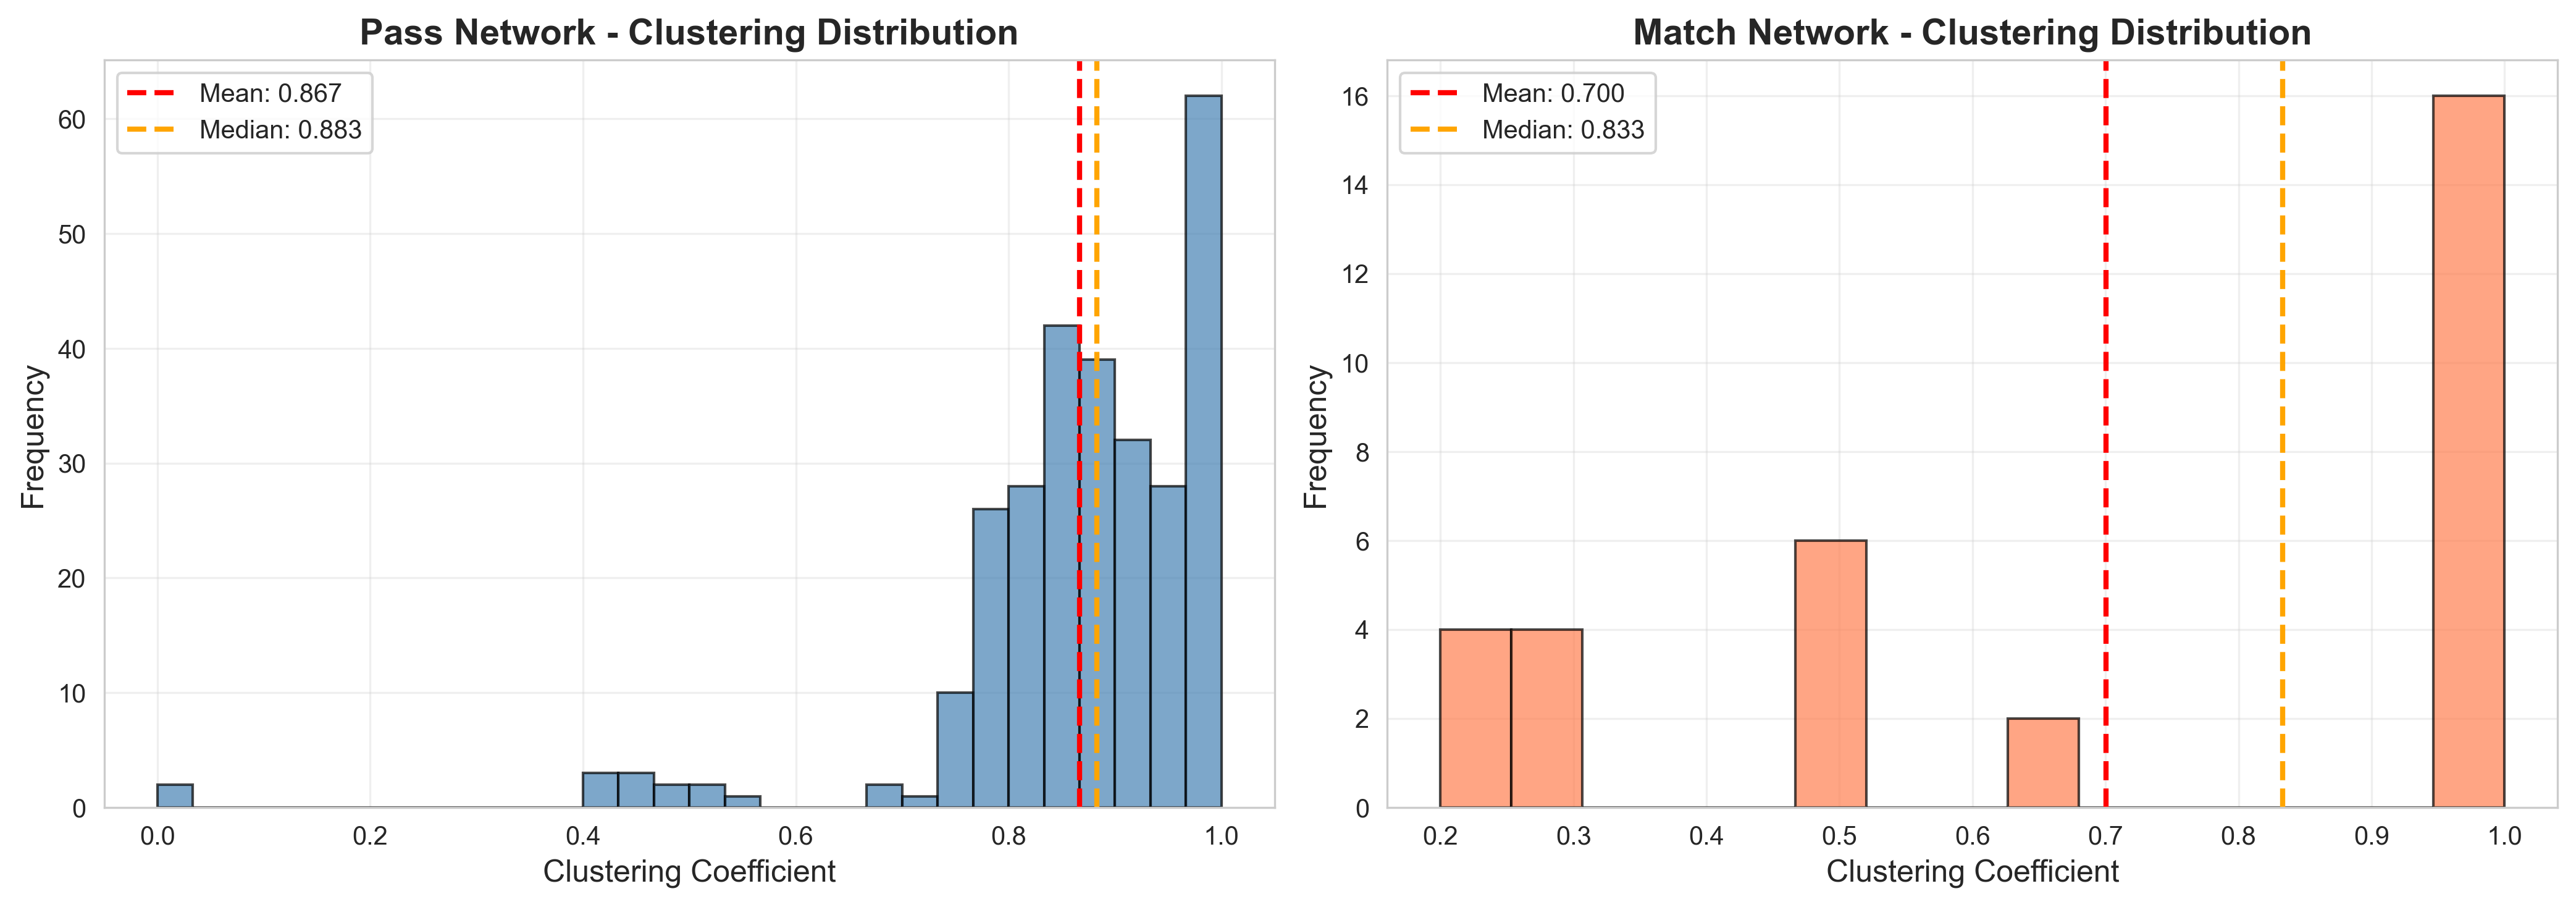
\includegraphics[width=0.95\linewidth]{figures/LE6/clustering_distribution.png}
  \caption{Verteilung des Clustering-Koeffizienten. Links: Pass-Netzwerk (hoch konzentriert um 0.8 - 0.9). Rechts: Match-Netzwerk (variierter).}
  \label{fig:clustering_distribution}
\end{figure}

\textbf{Interpretation:}
\begin{itemize}
  \item \textbf{Pass-Netzwerk}: Aussergewöhnlich hoher durchschnittlicher Clustering-Koeffizient (0.867) zeigt, dass Spieler in \textbf{eng vernetzten taktischen Einheiten} operieren. 81.6\% der Spieler haben $C_i \geq 0.8$, viele erreichen perfektes Clustering ($C_i = 1.0$). Dies reflektiert Positionsgruppen wie Verteidigungslinien oder Mittelfeld-Dreiecke.
  \item \textbf{Match-Netzwerk}: Hoher durchschnittlicher Clustering (0.700) reflektiert die Gruppenphase, in der Teams innerhalb einer Gruppe alle gegeneinander spielen.
\end{itemize}

\paragraph{Vergleich mit Zufallsnetzwerken}
In einem Zufallsnetzwerk mit gleicher Dichte gilt $C_{random} \approx \rho$ (Dichte). Vergleich:

\begin{table}[h]
\centering
\caption{Clustering vs. Zufallsnetzwerk}
\label{tab:clustering_vs_random}
\begin{tabular}{lccc}
\toprule
\textbf{Netzwerk} & \textbf{Clustering} & \textbf{Dichte} & \textbf{Ratio} \\
\midrule
Pass-Netzwerk & 0.8183 & 0.0727 & 11.26$\times$ \\
Match-Netzwerk & 0.4904 & 0.1270 & 3.86$\times$ \\
\bottomrule
\end{tabular}
\end{table}

Beide Netzwerke zeigen deutlich höheres Clustering als erwartet: Das Pass-Netzwerk hat \textbf{11.26-fach} höheres Clustering als ein äquivalentes Zufallsnetzwerk. Dies bestätigt stark strukturierte, nicht-zufällige Verbindungsmuster.

\begin{figure}[h]
  \centering
  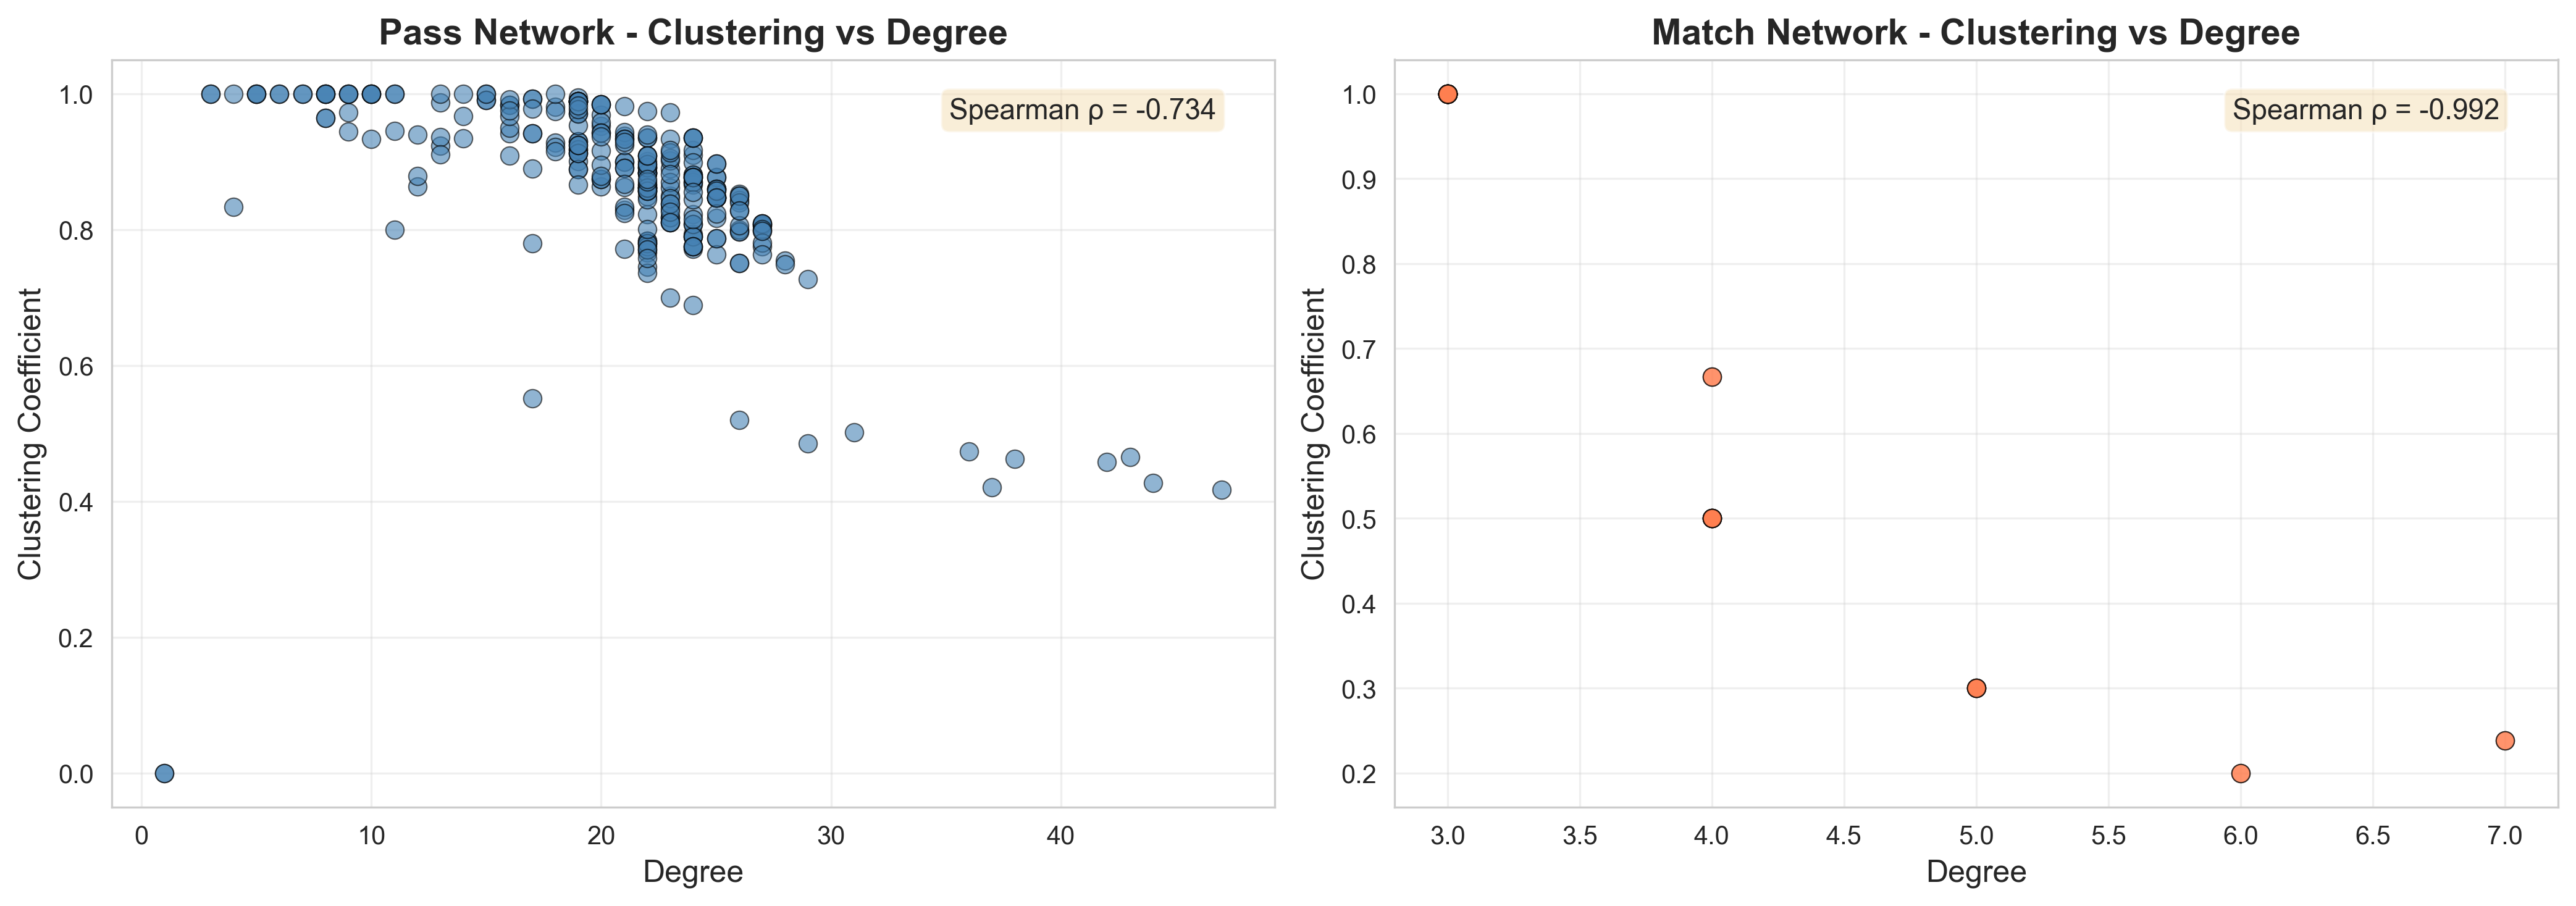
\includegraphics[width=0.95\linewidth]{figures/LE6/clustering_vs_degree.png}
  \caption{Clustering-Koeffizient vs. Degree. Pass-Netzwerk zeigt schwache negative Korrelation (Spearman $\rho = -0.235$), Match-Netzwerk schwache positive Korrelation ($\rho = 0.107$).}
  \label{fig:clustering_vs_degree}
\end{figure}

Die schwache negative Korrelation im Pass-Netzwerk deutet darauf hin, dass Spieler mit vielen Verbindungen (Hubs) tendenziell verschiedene Gruppen überbrücken und daher niedrigeres lokales Clustering aufweisen.

\paragraph{Small-World-Struktur}
Die Kombination von \textbf{niedrige Dichte} (0.073) + \textbf{hoher Clustering} (0.818) + \textbf{kurze Pfadlängen} (5.5) bestätigt die Small-World-Eigenschaft des Pass-Netzwerks: Spieler operieren in eng vernetzten taktischen Einheiten, während der Ball dennoch effizient über das gesamte Team fliessen kann.

\subsubsection{Assortativity}

\textbf{Assortativity} misst die Tendenz ähnlicher Knoten, sich zu verbinden. Die Degree-Assortativity ist die Pearson-Korrelation der Grade an Kantenendpunkten:
\begin{equation}
r = \frac{\text{cov}(k_i, k_j)}{\sigma_{k_i} \sigma_{k_j}}
\end{equation}

Wertebereich: $[-1, 1]$
\begin{itemize}
  \item $r > 0$: \textbf{Assortativ} (Hubs verbinden sich mit Hubs)
  \item $r < 0$: \textbf{Disassortativ} (Hubs verbinden sich mit peripheren Knoten)
  \item $r \approx 0$: Neutrales Mischen
\end{itemize}

\paragraph{Ergebnisse}

\begin{table}[h]
\centering
\caption{Degree-Assortativity}
\label{tab:assortativity}
\begin{tabular}{lc}
\toprule
\textbf{Netzwerk} & \textbf{Assortativity $r$} \\
\midrule
Pass-Netzwerk (ungerichtet) & 0.0062 \\
Pass-Netzwerk (In-Degree) & 0.0007 \\
Pass-Netzwerk (Out-Degree) & -0.0075 \\
Match-Netzwerk & 0.0891 \\
\bottomrule
\end{tabular}
\end{table}

\textbf{Interpretation:}
\begin{itemize}
  \item Beide Netzwerke zeigen \textbf{neutrales Assortativity} ($r \approx 0$), d.h. keine Präferenz für Verbindungen nach Grad-Ähnlichkeit.
  \item \textbf{Pass-Netzwerk}: Anders als in sozialen Netzwerken (oft assortativ, $r > 0.2$) zeigen Fussballteams keine Präferenz für Pässe zwischen Spielern ähnlichen Grades. Schlüsselspieler (Playmaker) passen sowohl zu anderen Kernspielern als auch zu peripheren Angreifern/Verteidigern, funktionale Integration statt Homophilie.
  \item \textbf{Match-Netzwerk}: Leicht positiv (0.089), aber neutral. Reflektiert Balance zwischen Gru\-ppenphase (gemischte Team-Stärken) und K.O.-Runden (ähnliche Performance-Level).
\end{itemize}

Vergleich mit anderen Netzwerktypen:
\begin{itemize}
  \item Soziale Netzwerke: typisch $r > 0.2$ (assortativ)
  \item Technologische Netzwerke: typisch $r < -0.2$ (disassortativ, Hub-and-Spoke)
  \item Fussballnetzwerke: $r \approx 0$ (aufgabenorientiert, keine Grad-Homophilie)
\end{itemize}

\subsubsection{Reciprocity}

\textbf{Reciprocity} $\rho_{recip}$ misst den Anteil bidirektionaler Kanten in gerichteten Netzwerken:
\begin{equation}
\rho_{recip} = \frac{|\{(i,j) : (i,j) \in E \land (j,i) \in E\}|}{|E|}
\end{equation}

Wertebereich: $[0, 1]$

\paragraph{Ergebnisse}

\begin{table}[h]
\centering
\caption{Reciprocity in gerichteten Netzwerken}
\label{tab:reciprocity}
\begin{tabular}{lccc}
\toprule
\textbf{Netzwerk} & \textbf{Reciprocity} & \textbf{Reziproke Kanten} & \textbf{Einseitige Kanten} \\
\midrule
Pass-Netzwerk (LCC) & 0.9269 & 5\,008 (92.7\%) & 395 (7.3\%) \\
Match-Netzwerk & 1.0000 & 126 (100\%) & 0 (0\%) \\
\bottomrule
\end{tabular}
\end{table}

\textbf{Interpretation:}
\begin{itemize}
  \item \textbf{Pass-Netzwerk}: Aussergewöhnlich hohe Reciprocity (92.7\%) zeigt, dass fast alle Passbeziehungen bidirektional sind. Dies reflektiert \textbf{kollaboratives, ballbesitzorientiertes Spiel}, in dem Spieler sich gegenseitig unterstützen. Die wenigen einseitigen Kanten (7.3\%) sind vermutlich spezialisierte Rollen (z.B. Zielspieler empfangen, passen aber selten zurück).
  \item \textbf{Match-Netzwerk}: Perfekte Reciprocity (100\%) ist eine strukturelle Eigenschaft: Jedes Spiel erzeugt eine bidirektionale Beziehung (Team A vs. Team B).
\end{itemize}

Vergleich mit anderen gerichteten Netzwerken:
\begin{itemize}
  \item Soziale Netzwerke (Twitter Follows): 20 - 40\% Reciprocity
  \item Informationsnetzwerke (Web Links): $<10\%$ Reciprocity
  \item Fussball Pass-Netzwerke: 92.7\% Reciprocity: reflektiert kooperative Natur des Teamsports
\end{itemize}

\subsection{Lokale Kennzahlen}

\subsubsection{Edge Embeddedness}

\textbf{Edge Embeddedness} $emb(i,j)$ zählt die gemeinsamen Nachbarn zweier verbundener Knoten:
\begin{equation}
emb(i,j) = |N(i) \cap N(j)|
\end{equation}

wobei $N(i)$ die Nachbarschaft von Knoten $i$ ist.

Kanten mit $emb(i,j) = 0$ werden \textbf{Local Bridges} genannt. Sie verbinden Gruppen ohne gemeinsame Nachbarn.

\paragraph{Ergebnisse}

\begin{table}[h]
\centering
\caption{Edge Embeddedness}
\label{tab:edge_embeddedness}
\begin{tabular}{lcccc}
\toprule
\textbf{Netzwerk} & \textbf{Ø Embeddedness} & \textbf{Median} & \textbf{Max} & \textbf{Local Bridges} \\
\midrule
Pass-Netzwerk (LCC) & 17.69 & 18 & 27 & 2 (0.1\%) \\
Match-Netzwerk & 1.62 & 2 & 3 & 12 (19.0\%) \\
\bottomrule
\end{tabular}
\end{table}

\begin{figure}[h]
  \centering
  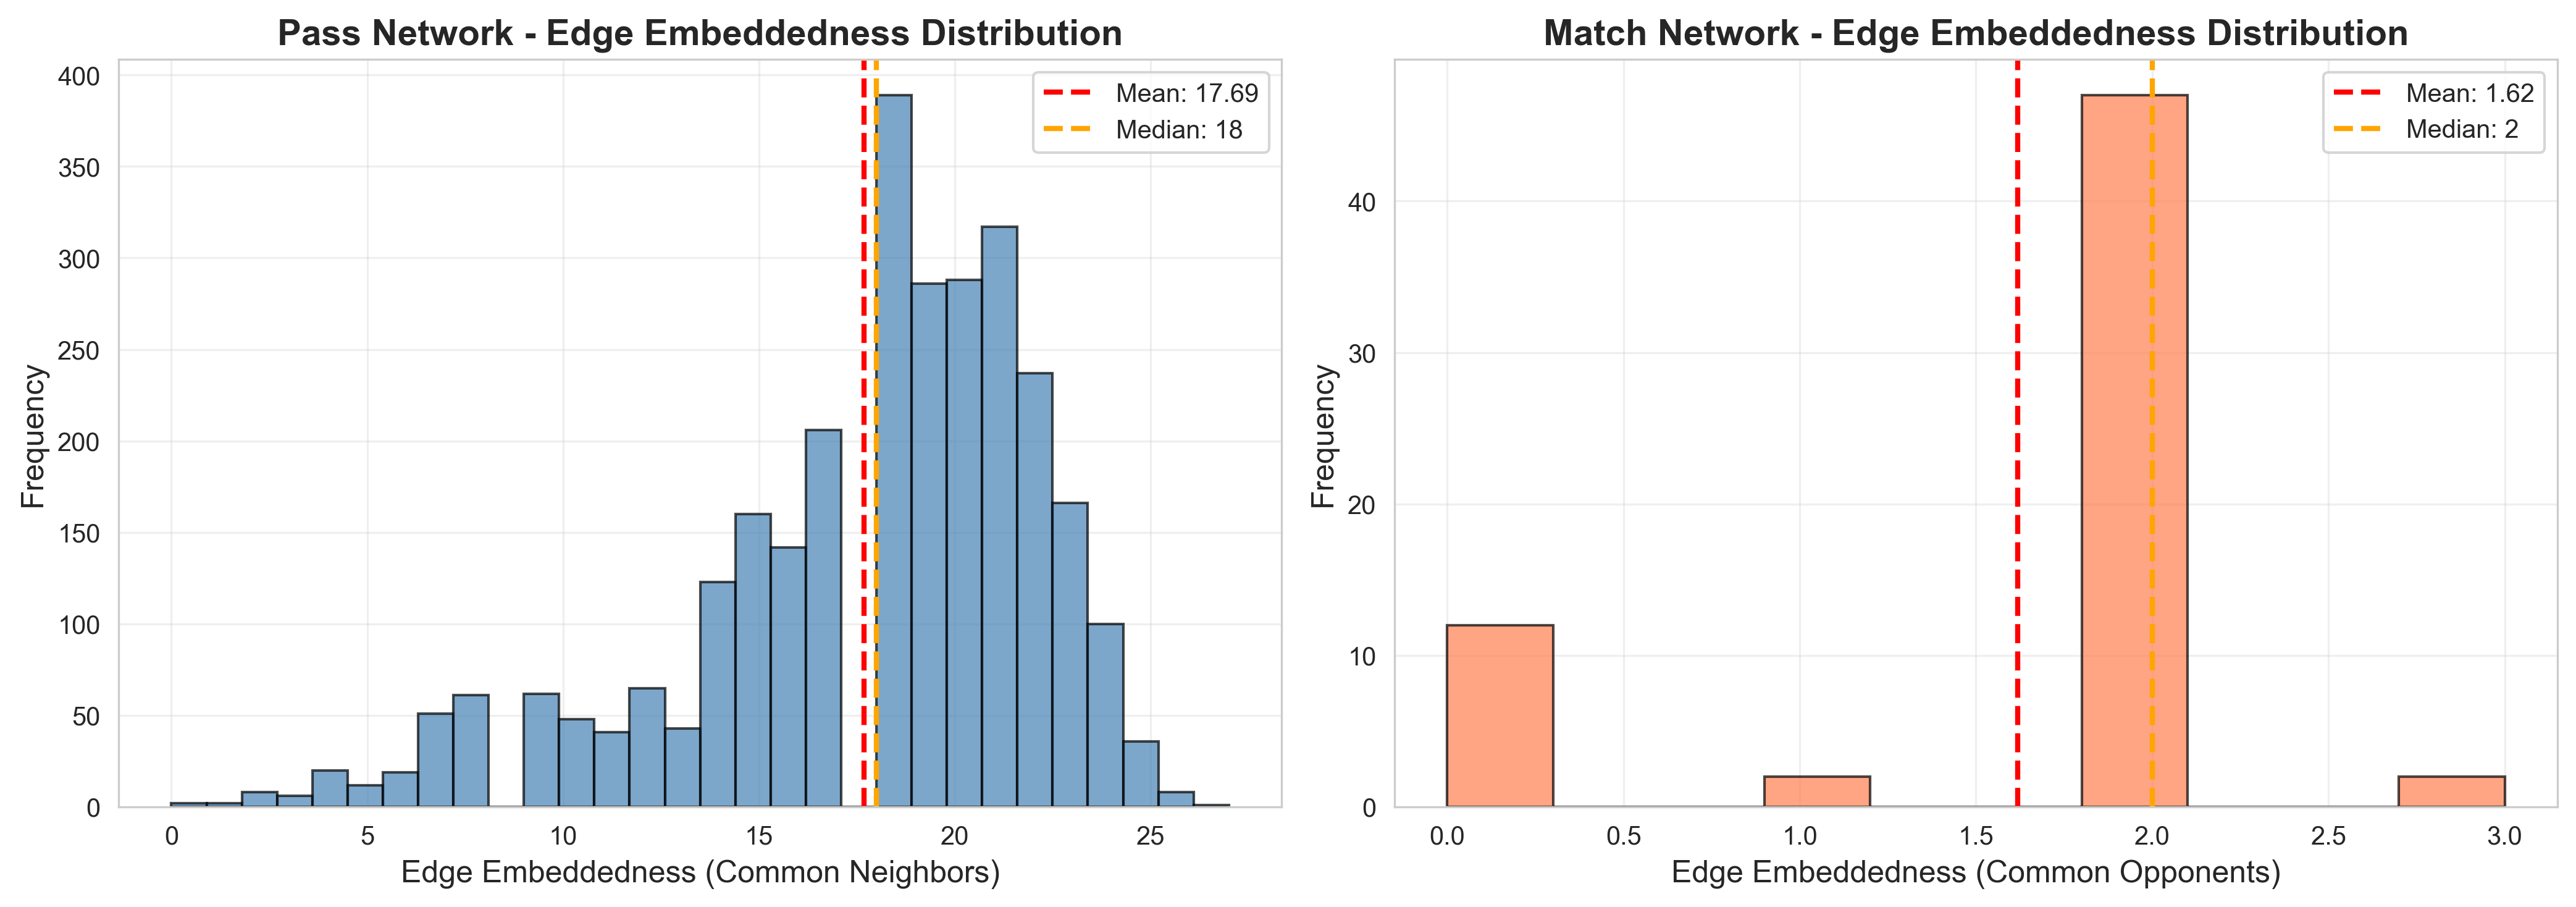
\includegraphics[width=0.95\linewidth]{figures/LE6/edge_embeddedness_distribution.png}
  \caption{Verteilung der Edge Embeddedness. Pass-Netzwerk zeigt hohe Einbettung (Ø 17.7 gemeinsame Nachbarn), Match-Netzwerk niedrige Einbettung (Ø 1.6).}
  \label{fig:edge_embeddedness}
\end{figure}

\textbf{Interpretation:}
\begin{itemize}
  \item \textbf{Pass-Netzwerk}: Aussergewöhnlich hohe Embeddedness (Ø 17.7) zeigt, dass Passbeziehungen \textbf{tief in taktischen Einheiten eingebettet} sind. Verbundene Spieler teilen durchschnittlich 18 gemeinsame Passpartner. Fast keine Local Bridges (nur 2, 0.1\%), praktisch jede Passverbindung hat multiple alternative Routen durch gemeinsame Nachbarn. Dies reflektiert \textbf{redundante taktische Struktur} mit vielfältigen Passoptionen.
  \item \textbf{Match-Netzwerk}: Niedrige Embeddedness (Ø 1.6) reflektiert die begrenzte Verbindung zwischen Turnieren.
  Teams teilen nur 2 gemeinsame Gegner im Durchschnitt. 12 Local Bridges (19\%) repräsentieren Paarungen zwischen Teams aus verschiedenen Gruppen oder Turnierphasen ohne Überlappung.
\end{itemize}

Die Verteilung zeigt (siehe Abb.~\ref{fig:edge_embeddedness}):
\begin{itemize}
  \item Pass-Netzwerk: 91.6\% der Kanten haben $emb \geq 10$, hochredundante Struktur
  \item Match-Netzwerk: Maximum nur 3 gemeinsame Gegner, strukturell begrenzte Überlappung
\end{itemize}

\subsection{Zusammenfassende Analyse}

\begin{table}[h]
\centering
\caption{Umfassende Netzwerk-Metriken (Zusammenfassung)}
\label{tab:comprehensive_metrics}
\resizebox{\textwidth}{!}{%
\begin{tabular}{lcc}
\toprule
\textbf{Metrik} & \textbf{Pass-Netzwerk (LCC)} & \textbf{Match-Netzwerk} \\
\midrule
Knoten & 283 & 32 \\
Kanten & 2\,899 & 63 \\
Dichte & 0.0727 & 0.1270 \\
Diameter & 13 & 6 \\
Avg Path Length & 5.476 & 3.163 \\
Avg Clustering Coef & 0.8667 & 0.7003 \\
Transitivity & 0.8183 & 0.4904 \\
Anzahl Dreiecke & 17\,093 & 34 \\
Avg Edge Embeddedness & 17.69 & 1.62 \\
Assortativity & 0.0062 & 0.0891 \\
Reciprocity & 0.9269 & 1.0000 \\
Small-World Ratio & 0.97 & 0.91 \\
\bottomrule
\end{tabular}%
}
\end{table}

\begin{figure}[h]
  \centering
  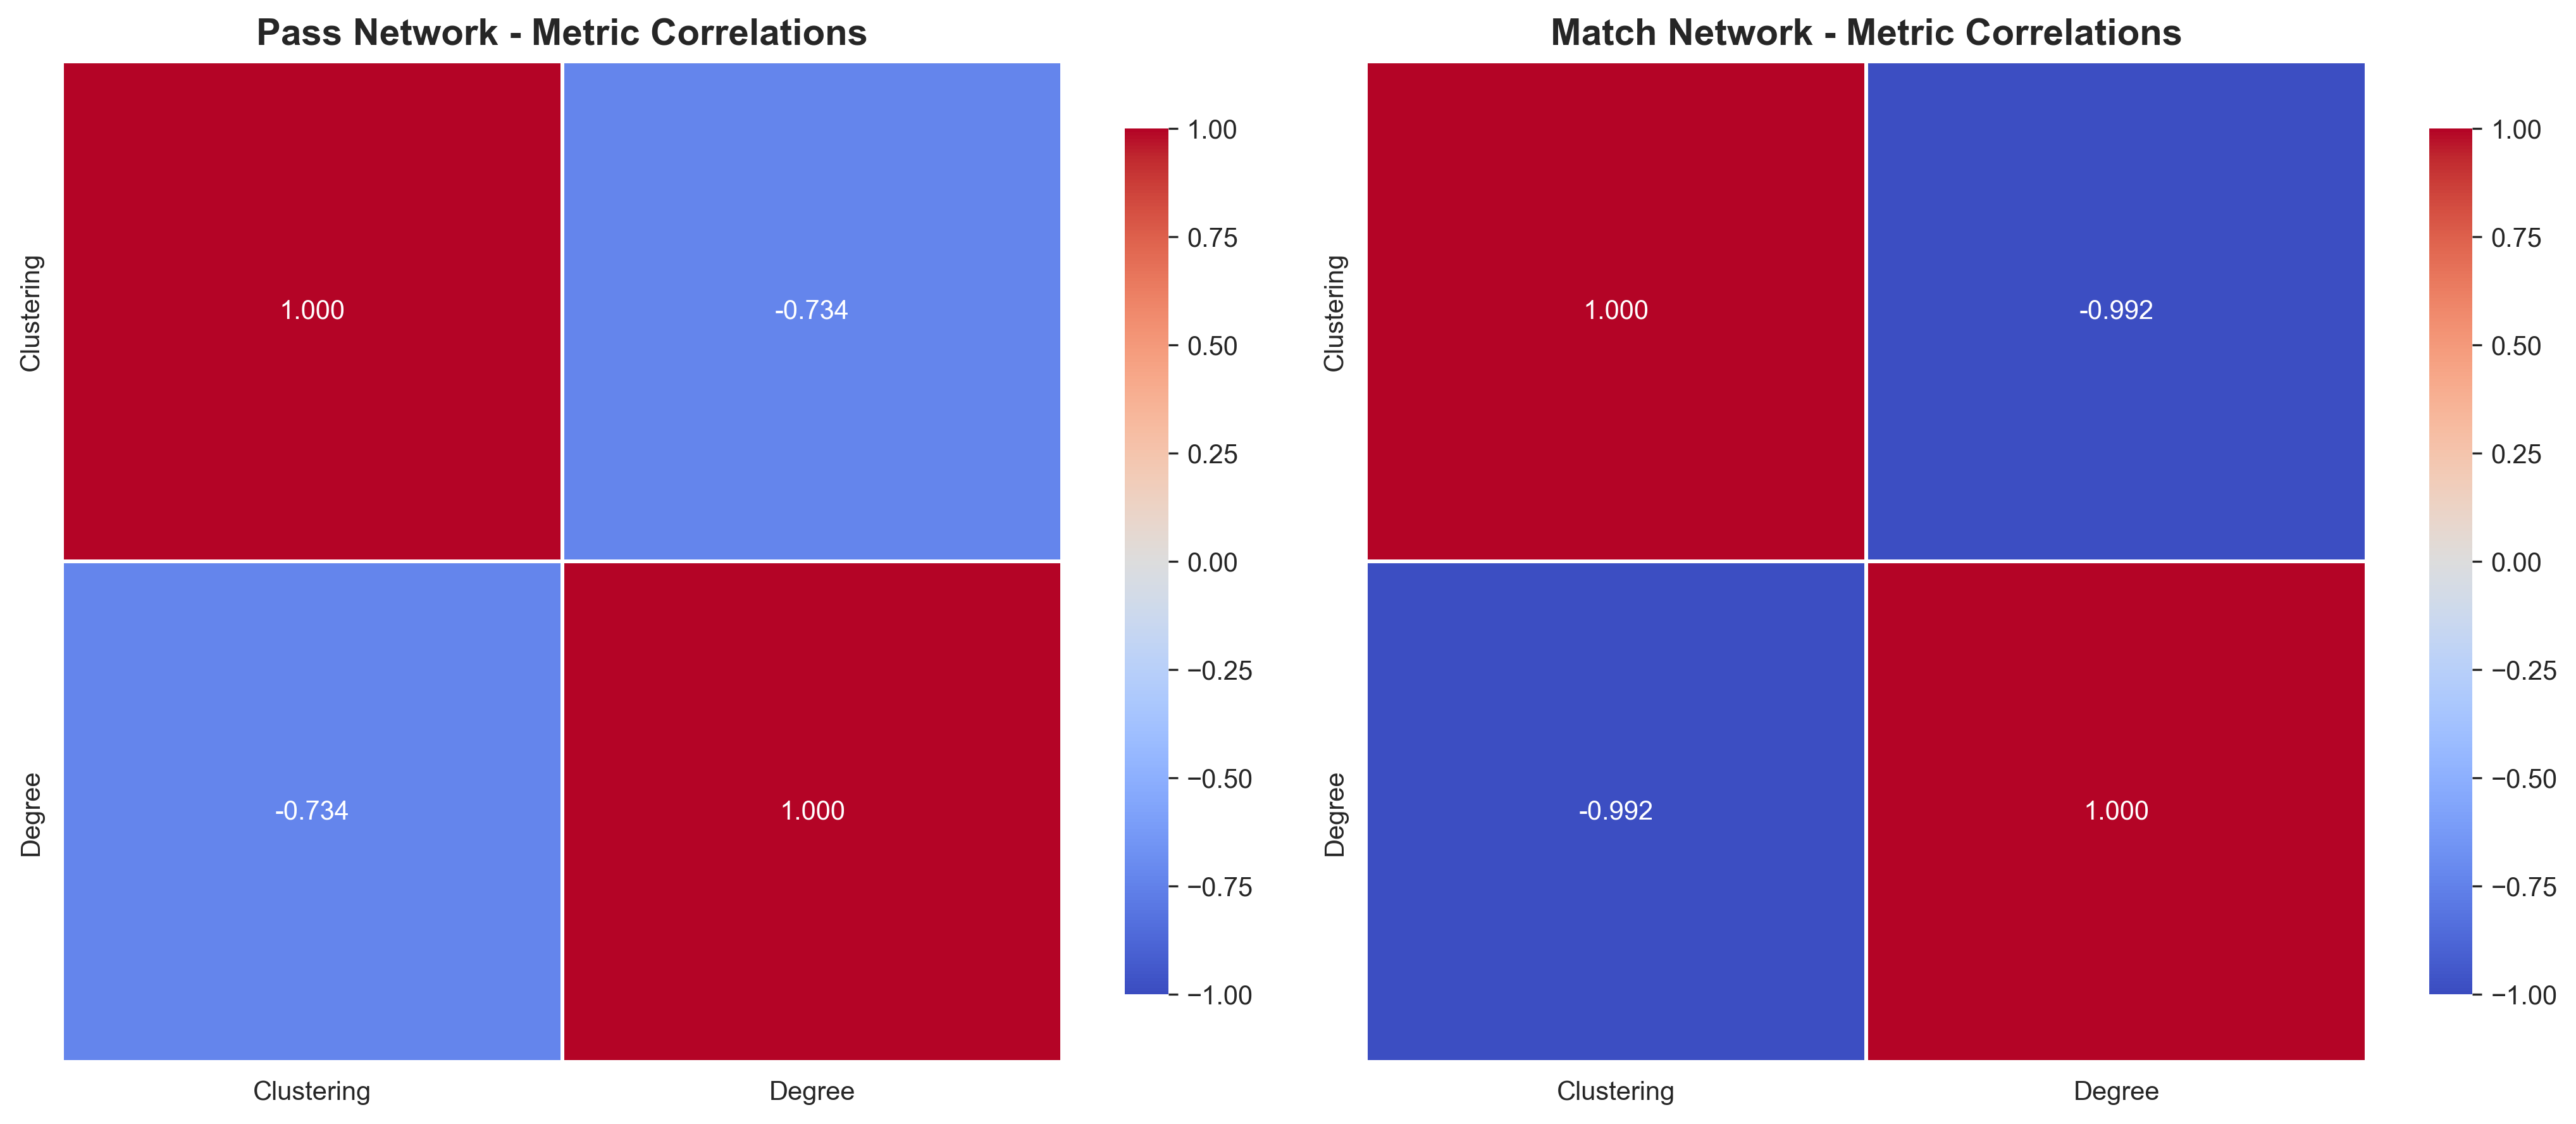
\includegraphics[width=0.8\linewidth]{figures/LE6/metric_correlations.png}
  \caption{Korrelationen zwischen Metriken. Links: Pass-Netzwerk zeigt schwache negative Korrelation zwischen Clustering und Degree ($\rho = -0.235$). Rechts: Match-Netzwerk zeigt schwache positive Korrelation ($\rho = 0.107$).}
  \label{fig:metric_correlations}
\end{figure}

\subsubsection{Strukturelle Unterschiede}

\paragraph{1. Skala \& Konnektivität}
\begin{itemize}
  \item Pass-Netzwerk ist 8.8-fach grösser (283 vs. 32 Knoten)
  \item Aber 1.7-fach weniger dicht (0.073 vs. 0.127)
  \item Grössere Netzwerke können niedrigere Dichte mit hoher Konnektivität kombinieren
\end{itemize}

\paragraph{2. Lokale Struktur (Clustering \& Embeddedness)}
\begin{itemize}
  \item Pass-Netzwerk: 1.7-fach höheres Clustering (0.818 vs. 0.490)
  \item Pass-Kanten 10.9-fach stärker eingebettet (17.7 vs. 1.6 gemeinsame Nachbarn)
  \item \textbf{Pass-Netzwerk}: Eng vernetzte taktische Einheiten mit redundanten Verbindungen
  \item \textbf{Match-Netzwerk}: Spärliche Turnierstruktur mit begrenzter Überlappung
\end{itemize}

\paragraph{3. Globale Struktur (Distanz \& Diameter)}
\begin{itemize}
  \item Pass-Netzwerk hat längere Pfade (Ø 5.5 vs. 3.2)
  \item Beide erfüllen Small-World-Eigenschaft (Ratio $\approx 1$)
  \item Effizient trotz unterschiedlicher Grössen
\end{itemize}

\paragraph{4. Mischungsmuster}
\begin{itemize}
  \item Beide zeigen neutrales Assortativity ($\approx 0$): keine Grad-Homophilie
  \item Beide zeigen hohe Reciprocity (92.7\% Pass, 100\% Match)
  \item \textbf{Pass-Netzwerk}: Kollaboratives ballbesitzorientiertes Spiel
  \item \textbf{Match-Netzwerk}: Round-Robin-Turnierstruktur
\end{itemize}

\paragraph{5. Netzwerktypen}
\begin{itemize}
  \item \textbf{Pass-Netzwerk}: Small-World mit hohem Clustering + niedriger Dichte
  \item \textbf{Match-Netzwerk}: Dichter Turniergraph mit moderatem Clustering
\end{itemize}

\subsection{Diskussion}

\subsubsection{Small-World-Eigenschaften in Fussballnetzwerken}

Die Analyse bestätigt, dass beide Netzwerke \textbf{Small-World-Eigenschaften} aufweisen: kurze Pfadlängen (Effizienz) kombiniert mit hohem Clustering (lokale Struktur). Diese Kombination ist charakteristisch für gut organisierte Systeme.

Im \textbf{Pass-Netzwerk} bedeutet dies:
\begin{itemize}
  \item Spieler operieren in eng vernetzten taktischen Einheiten (Verteidigung, Mittelfeld, Angriff)
  \item Gleichzeitig ermöglicht die Gesamtstruktur schnellen Ballfluss über das gesamte Team
  \item Niedriger Diameter trotz hohem Clustering, optimale Balance zwischen Spezialisierung und Integration
\end{itemize}

\subsubsection{Taktische Implikationen}

Die Metriken offenbaren wichtige taktische Muster:

\paragraph{Redundante Passoptionen}
Hohe Edge Embeddedness (Ø 17.7 gemeinsame Nachbarn) zeigt, dass Teams \textbf{multiple Passoptionen} aufbauen. Wenn ein direkter Pass blockiert ist, existieren viele alternative Routen durch gemeinsame Nachbarn. Dies ist charakteristisch für Ballbesitz-orientierte Taktiken (z.B. Tiki-Taka).

\paragraph{Kollaboratives Spiel}
Sehr hohe Reciprocity (92.7\%) bestätigt, dass erfolgreiches Passspiel auf \textbf{gegenseitiger Unterstützung} basiert. Spieler bieten sich kontinuierlich als Anspielstationen an und schaffen dadurch natürliche bidirektionale Passoptionen.

\paragraph{Funktionale Integration}
Neutrales Assortativity ($r \approx 0$) zeigt, dass Schlüsselspieler (hoher Degree) nicht präferenziell untereinander passen, sondern das gesamte Team integrieren. Dies unterscheidet Fussball von sozialen Netzwerken und reflektiert die \textbf{aufgabenorientierte Natur} des Sports.

\subsubsection{Limitationen}

\paragraph{Statische Perspektive}
Alle Metriken basieren auf statischen, aggregierten Netzwerken. Dynamische Aspekte (wie sich Metriken während eines Spiels ändern) werden nicht erfasst.

\paragraph{Passempfänger-Identifikation}
Unsere Passempfänger-Zuordnung basiert auf raum-zeitlichem Matching (nächster Spieler innerhalb 5 Sekunden, 10 Meter). Fehlzuordnungen können Metriken beeinflussen, insbesondere:
\begin{itemize}
  \item Clustering könnte leicht überschätzt sein (falsche Dreiecke)
  \item Reciprocity robust (aggregierte Muster weniger anfällig)
\end{itemize}

\paragraph{Qualitative Aspekte}
Metriken berücksichtigen nicht die \textbf{Qualität} von Aktionen:
\begin{itemize}
  \item Erfolgreiche vs. erfolglose Pässe
  \item Pässe unter Druck vs. freie Pässe
  \item Rückwärtspässe vs. progressive Pässe
\end{itemize}

\subsection{Fazit}

Die Netzwerk-Kennzahlen offenbaren fundamentale strukturelle Eigenschaften unserer Fussballnetzwerke:

\begin{enumerate}
  \item \textbf{Small-World-Struktur}: Beide Netzwerke kombinieren kurze Pfadlängen (Effizienz) mit hohem Clustering (lokale Struktur)
  \item \textbf{Taktische Organisation}: Aussergewöhnlich hoher Clustering (0.818) und Embeddedness (17.7) zeigen eng vernetzte taktische Einheiten
  \item \textbf{Redundanz}: Multiple Passoptionen durch gemeinsame Nachbarn, charakteristisch für Ballbesitz-Taktiken
  \item \textbf{Kollaboration}: Sehr hohe Reciprocity (92.7\%) reflektiert gegenseitige Unterstützung im Passspiel
  \item \textbf{Funktionale Integration}: Neutrales Assortativity zeigt aufgabenorientierte Vernetzung ohne Grad-Homophilie
\end{enumerate}

Diese Erkenntnisse sind sowohl für deskriptive Netzwerkanalyse als auch für strategische Überlegungen relevant. Die Metriken ermöglichen quantitative Vergleiche zwischen Teams, Ligen oder taktischen Systemen und können als Basis für Performance-Analysen dienen.

\textbf{Ausblick}: Zukünftige Analysen könnten dynamische Metriken (Veränderung während eines Spiels), positions-spezifische Kennzahlen oder den Einfluss von Metriken auf Spielergebnisse untersuchen.

\section{LE7 -- Statistik in Netzwerken}

\subsection{Ziel}
\textit{Welche statistischen Fragestellungen werden am Netzwerk untersucht? (Hypothesentests, Modelle, Signifikanz)}

\subsection{Nullmodelle \& Randomisierung}
\begin{itemize}
  \item Konfigurationsmodell / Degree-preserving Randomization
  \item Permutationstests / Bootstrap
  \item Vergleich beobachtet vs. erwartet (z.B. Clustering, Pfadl\"ange)
\end{itemize}

\subsection{Modelle}
\begin{itemize}
  \item ERGM / St\"arkere Modelle (falls genutzt)
  \item Regression mit Netzwerkmerkmalen
\end{itemize}

\subsection{Ergebnisse}
\textit{Berichte Teststatistiken, Konfidenzintervalle und Interpretation.}

\section{LE8 -- Link Prediction}

\subsection{Ziel}
\textit{Welche Kanten sollen vorhergesagt werden (zeitlich oder als fehlende Links)?}

\subsection{Features / Heuristiken}
\begin{itemize}
  \item Common Neighbors, Jaccard, Adamic--Adar
  \item Preferential Attachment
  \item Katz / Rooted PageRank
  \item Einbettungen (z.B. node2vec) oder GNN (falls genutzt)
\end{itemize}

\subsection{Evaluation}
\begin{itemize}
  \item Train/Test Split (z.B. zeitbasiert), Negative Sampling
  \item Metriken: AUC, Average Precision, Precision@k
  \item Baselines und Ablations
\end{itemize}

\subsection{Ergebnisse}
\textit{Vergleiche Methoden, diskutiere Fehlerf\"alle und praktische Aussagekraft.}

\section{LE9 -- Diffusion}

\subsection{Ziel}
\textit{Welche Diffusionsprozesse werden modelliert oder simuliert? (Information, Krankheit, Adoption, ...)}

\subsection{Modelle}
\begin{itemize}
  \item SI/SIR/SIS oder Threshold/Independent Cascade
  \item Parameter (Infektionsrate, Recovery, Schwellen)
  \item Seed-Strategien (zufällig, hochgradig, zentral nach LE5)
\end{itemize}

\subsection{Simulation \& Auswertung}
\begin{itemize}
  \item Mehrere Läufe und Unsicherheit
  \item Messgrößen: Endgröße, Geschwindigkeit, Reach, Time-to-\dots
\end{itemize}

\subsection{Ergebnisse}
\textit{Vergleiche Modelle/Parameter und diskutiere Implikationen.}

\section{LE10 -- Graphlets}

\subsection{Ziel}
\textit{Welche lokalen Strukturen (Graphlets/Motive) sollen gezählt oder verglichen werden?}

\subsection{Vorgehen}
\begin{itemize}
  \item Graphlet-Größe $k$ (z.B. 3--5) und Wahl der Typen
  \item Zählverfahren / Sampling (falls nötig)
  \item Normalisierung und Vergleich (z.B. Graphlet Degree Vector, Orbit Counts)
\end{itemize}

\subsection{Ergebnisse}
\textit{Zeige dominante Graphlets, Unterschiede zwischen Subnetzen/Communities oder über Zeit, und interpretiere diese.}


%%---BIBLIOGRAPHY------------------------------------------------------------------------
{\sloppypar
\printbibliography[heading=bibintoc, title=Quellenverzeichnis]
}

\end{document}
